\graphicspath{{imgs/}}

%===============================================================================
\chapter{Introduction}
%===============================================================================
%
Throughout my academic career, I have enjoyed the step-by-step process of learning and I have discovered a passion for sharing my knowledge with friends, colleagues and some of my students.
In the same way the process of learning is unique, the process of teaching or communicating the knowledge should also be personal, trying to achieve the main goal of communication, transmitting correct information.
When we try to learn about a subject we can go to books, classes, different teachers, publications..., and sometimes we understand better from a book, other times from a video or a specific teacher or friend.
In this thesis, I will present some results on the physics of turbulent fluid mechanics where I have been involved, and I will try my best to communicate this knowledge to those interested in reading this work even if the reader is not very familiar with fluid dynamics.
Ideally, this transmission of knowledge should be concise, but I have experienced that certain complex knowledge sometimes requires different points of view or a simpler language. Personally, I like to communicate my knowledge as if it was a conversation instead of formal and impersonal writing.

Fluid mechanics or dynamics may sound as something complex for the non initiated, and it really is a complex science, but we already have intuitive and practical knowledge since we live and manipulate fluids every day so I will explain the basics.

A fluid is a substance that in contrast with a solid, it can easily deform and this property allows for the substance to adapt to containers or to move around other obstacles. An example is the air of the atmosphere, the liquid water in the sea, and even solids, like large accumulations of fine sand which subjected to vibrations can behave similar to liquid water.
Fluid mechanics is the science that studies everything related to the movement of fluids, like the forces involved or the properties of the fluid in its motion.

When a fluid moves around a solid (water around a rock), or the solid moves immersed in a fluid  (car moving through the air of the atmosphere) the fluid adapts to that relative motion by changing its properties, such as the velocity of its particles.
Where the fluid meets the solid, its particles have the same velocity as the solid because the forces in the interface fluid-solid (friction and pressure forces) are enough to deform the fluid.
The viscosity is the property of the fluid that opposes to the deformation. Inside the fluid, the viscosity is seeing as a force that reduces the velocity of the deformation or the velocity of the fluid particles.
In the example of the water in a river moving around a rock, far from the rock, the velocity of the water is that of the river, however the water in contact to the rock is not moving according to what we have explained earlier. The viscosity is responsible to adapt the velocity of the fluid from the velocity of the river to the velocity of the rock.
The change of velocity is actually done in a very small distance, and this region where the viscosity forces are adapting the fluid velocity is called boundary layer. 
The idea of boundary layer was introduced by Ludwig Prandtl in 1904 and it is the main topic of this thesis.

The boundary layers studied here are those pertaining to the momentum of the flow. The interest is in the effects of adverse pressure gradients in well-developed turbulent boundary layers. To avoid the influence of other effects we consider the simplest scenario.
The fluid is isotropic, incompressible and Newtonian, therefore the temperature does not change the density and the viscosity of the fluid.

The simplest solid boundary used is a flat plate without any heat or mass exchange (no suction or blowing). The adverse pressure gradient is then imposed as an outer boundary condition.
Comparisons can then be done with curved-boundary solids such as NACA profiles, where the pressure gradients are an aftereffect of the curvature of the profile. 
In these realistic configurations different mechanisms to control the flow are applied such as blowing or suction.

For these simple configurations we use a Cartesian system of coordinates where the space is denoted with $\vec{x}=x_i=(x,y,z)$, where we show the vectorial, dyadic and coordinate notations that will be used.
The boundary layers studied here are statistically 2D, $y$ is the wall-normal direction, $z$ is the homogeneous direction and $x$ is chosen as the streamwise direction. The time is denoted with $t$.
Although turbulence is a 3-dimensional (3D) phenomena, the flow analysed is statistically 2-dimensional, since there is an homogeneous direction. 

%-------------------------------------------------------------------------------
\section{Our Contribution}
%


\thesisstructure Add here a brief description of the structure of the thesis.

%===============================================================================
\chapter{Boundary layers, turbulence and pressure gradients}
%===============================================================================
%
% \begin{enumerate}
%     \item Physical phenomena
%     \begin{enumerate}
%         \item Elements involved (fluid and solid)
%         \item Properties of the elements that are meaningful for the problem
%         \item Observations or experimental knowledge $\rightarrow$ effects observed
%         \item New unseen problem $\rightarrow$ hypothesis of the effects to be observed
%     \end{enumerate}
    
%     \item Abstraction of the problem at hand and the physics
%     \begin{enumerate}
%         \item Equations for the physics studied (mechanics, thermal?, chemical?)
%         \item Mathematical model of the elements properties
%         \item Outer factors or conditions
%     \end{enumerate}
%     \item Analytical solution or numerical discretization.
%     \item Validation with experimental results
% \end{enumerate}

\graphicspath{{imgs/} {imgs/lam_turb} {imgs/spec}}

\section{Observations and empirical knowledge}

There are many examples of laminar and turbulent flows in nature that we are familiar with. In Fig.~\ref{fig:lam_turb} we show 3 examples, with water and flames. In the river image the water on the right side is laminar and on the left side it becomes turbulent. The calm flames of a candle rise initially in a laminar regime. On the bonfire example the flames are larger and show the different chaotic scale motions of a turbulent flow.

\begin{figure}[h!]
\centering
% \captionsetup{width=0.99 \textwidth}
\includegraphics[height=5cm ]{laminar_turbulent_1.jpg}
% \includegraphics[width=5cm ]{llama_laminar.jpg}
\includegraphics[height=5cm ]{velas.jpg}
\includegraphics[height=5cm ]{llama_turb1.jpg}
\caption{ \label{fig:lam_turb} Examples of ordered laminar flow and chaotic turbulent motions in water and fire.
   }
\end{figure}

Laminar and turbulent regimes presents its advantages and disadvantages. 
In aerodynamic applications we usually focus in minimizing the friction produced at the solid wall-boundary or maximizing the lift/drag coefficient. In that aspect, the laminar boundary layer produces less friction than a turbulent boundary layer because it alters less the flow.
Detachment of the flow is an undesirable effect produced by strong adverse-pressure gradients, in this aspect, the laminar flow structure is more sensible to detachment under APG conditions than a turbulent flow.

To study turbulent boundary layers (TBLs) and the effects of adverse pressure gradients (APG) we will compare APG TBLs with a TBL subjected to zero pressure gradient (ZPG) conditions. The case of favourable pressure gradients (FPGs) stabilizes and relaminarizes the boundary layer, and its effects are not critical such as those provoked by APGs, where the boundary layer can detach from the wall producing undesirable effects such as an increase in drag or even to loose the aerodynamic controls in airplanes.
In order to study this kind of wall-attached fluid problem, first we should analyze the elements involved, such as the fluid and the solid elements.

\section{Fluid properties}

When studying the mechanics of a solid we track the positions, velocities and accelerations, forces and torques along its movement in space and time. This is the Lagrangian approach to mechanics.
For a flow of particles or a fluid it is more interesting to observe the flow variables at specific locations and observe the temporal change of those variables at those locations. This is the Eulerian approach that will be used to study the mechanics of a fluid flow. 

The main variables are the fluid velocities, $\vec{u}(\vec{x},t)=u_i=(u,v,w)$, and the pressure $p(\vec{x},t)$.
To simplify the study of adverse pressure gradient turbulent boundary layers the fluid analysed is isotropic (its properties are the same in all directions) and Newtonian, this implies that the viscous forces are a linear function of the strain rate tensor $s_{ij}=\pdv{u_i}/{x_j}$. As an example, the friction at the wall is $\tau_w=\mu \pdv{u}/{y}$
where $\mu$ is a constant factor, the dynamic viscosity.
The density and viscosity of the fluid combines into the kinematic viscosity $\nu=\mu/\rho$ with units $[m^2/s]$ independent of the mass. 
Since we consider the density and viscosity as constant and not affected by changes in temperature, the temperature of the fluid is not relevant and the energy and momentum evolution are decoupled.

\section{Solid properties}
In general, the solid boundaries are curved specially in aerodynamic applications where the curvatures are used to create differences in pressures that lead to forces in the desired directions. The forces in the direction of the inflow are called drag and the forces in the perpendicular direction is called lift. For curved boundaries, different coordinate systems are used. The local system of coordinates that changes with the solid boundary is where the surface forces are calculated. The surface forces are then projected onto the global coordinates associated with the inflow to obtain the lift and drag.
For flat plates with zero angle of attack the global and local coordinates are the same.
The surface of the flat plate that we study is rigid, and smooth, and no exchange of heat or mass is produced between the fluid and the solid. In the interface fluid/solid the only interaction is due to pressure and viscous forces that adapts the fluid velocity to the solid surface velocity.
The flat plate will be considered to be static in the global system of coordinates.


\section{Boundary layers}

Boundary layers are regions inside a fluid flow where certain features or changes in the properties of the fluid are concentrated. Historically the first idea of boundary layer is set for the adaptation region of the fluid momentum from outer conditions to the dynamical conditions in a solid surface.
Other boundary layers are for example thermal boundary layers where the focus is on the change of thermal properties.

When we consider the flow around a solid object in an incompressible regime, the flow can detect the presence of the solid object and adapt its trajectory. The flow then surrounds the solid starting from the leading edge and close to the solid surface the boundary layer is the region where the velocity of the flow adapts from the solid surface velocity to the outer flow velocity. The boundary layer thickness have to be defined according to the main idea of a region of the fluid close to the solid wall that encloses the major viscous effects created due to the fluid/surface interaction. An obvious effect of the presence of a wall is that the streamwise velocity has to adapt from the velocity of the solid boundary to the exterior velocity, commonly called velocity at the infinity $U_{\infty}$. 
In general, for a certain position of the wall, the velocity is measured in the wall-normal direction, obtaining a profile of streamwise velocities $u(y,t)$. Then $U_{\infty}=u(y\rightarrow \infty)$ is the unperturbed velocity and can change from one streamwise position to another.
In the case of zero-pressure gradient boundary layers, $U_{\infty}$ is taken as constant, since in a steady flow in the absence of viscous forces, $\pdv{u}/{x}$ should be zero. 

Since an obvious indicator of the boundary layer is the adaptation of the streamwise velocity, the boundary layer can be defined using this property and the $99\%$ thickness $\delta_{99}$ is defined as the wall-normal position where $u(y=\delta_{99}) = U_{\infty}$.
In Fig.~\ref{fig:lam_turb_profiles} we show an example on how the mean streamwise velocity $U(y)$ adapts from the velocity at the wall $u(y=0)=0$, to the outer velocity $U_{\infty}$, which has been scaled to be equal to 1, on a laminar and a TBL ZPG profiles.

\begin{figure}[h!]
\centering
% \captionsetup{width=0.99 \textwidth}
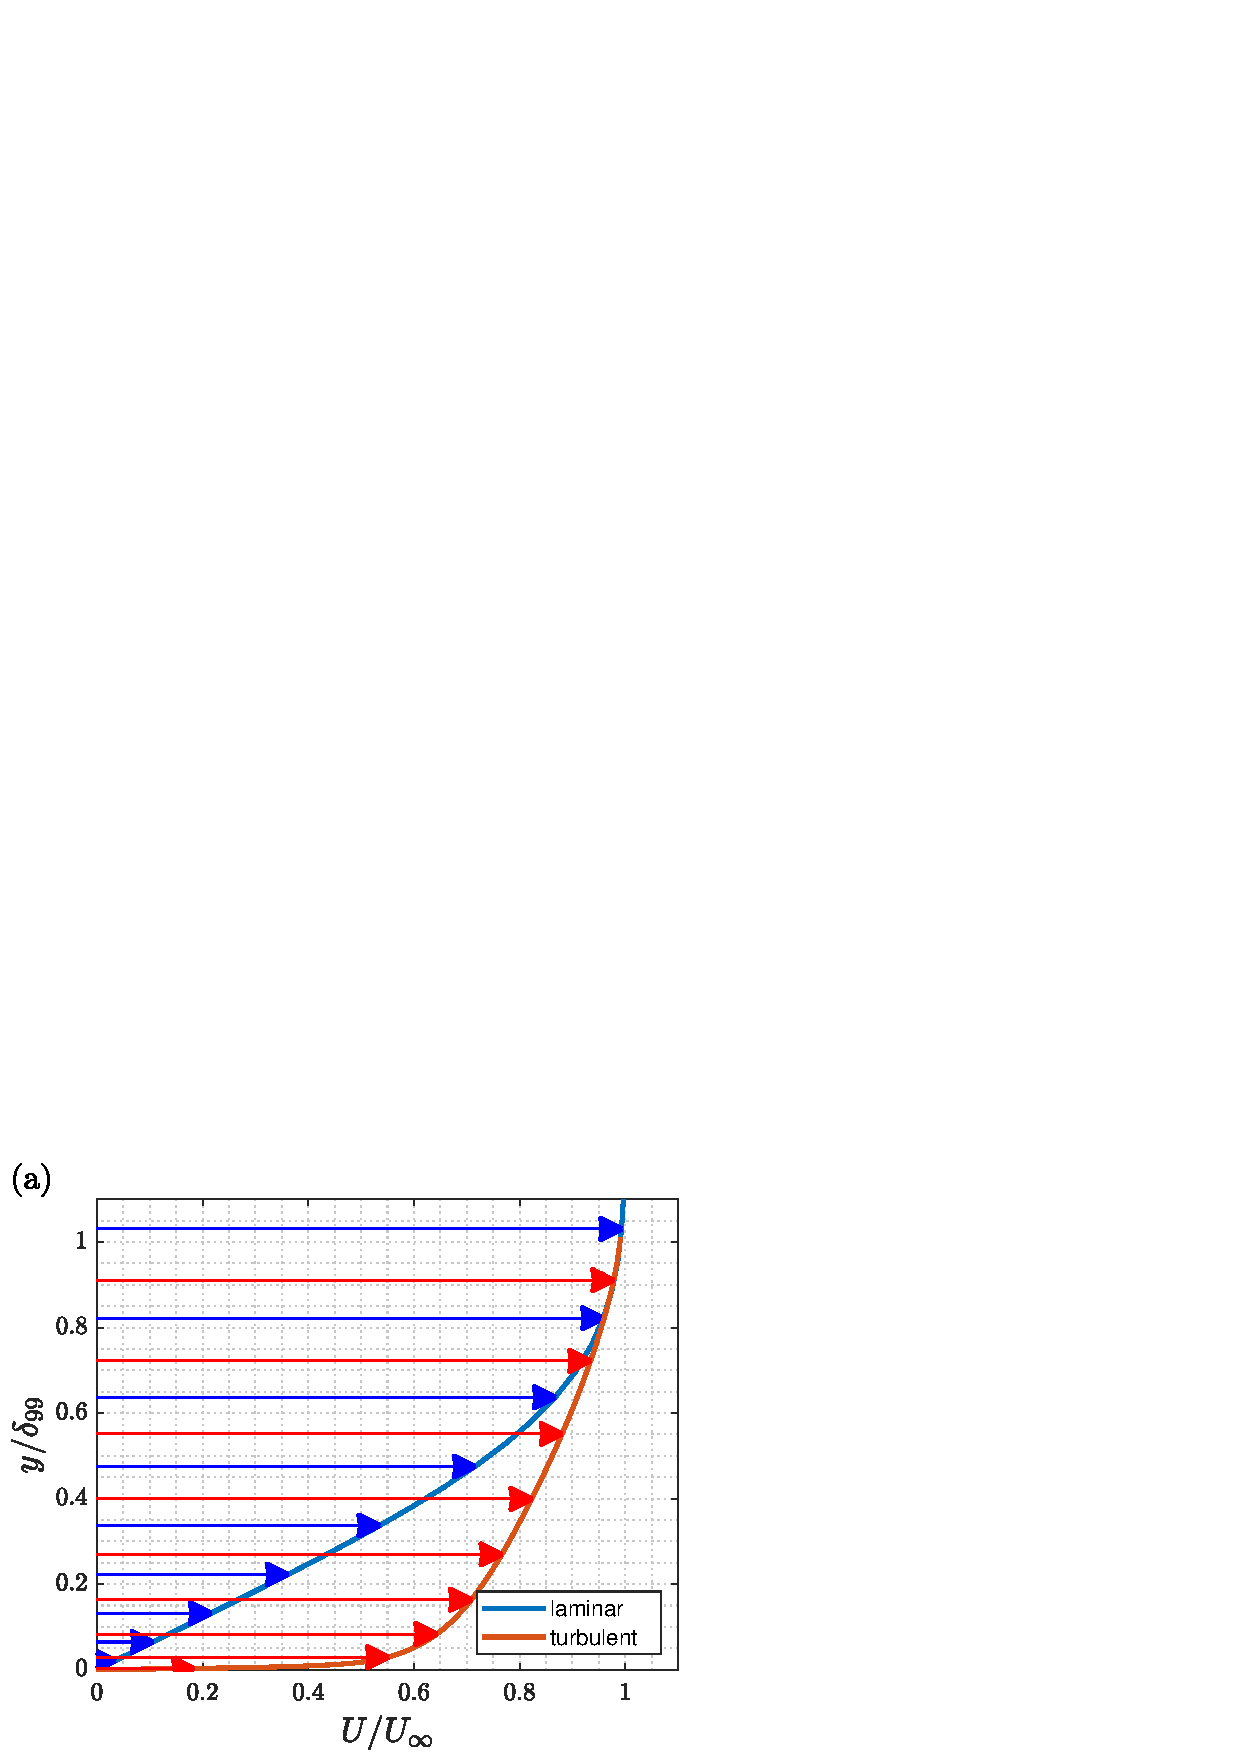
\includegraphics[width=0.5\textwidth]{ZPG_lam_turb.jpg}
\caption{ \label{fig:lam_turb_profiles} Mean streamwise velocity profile of a laminar (blue) and a turbulent ZPG (red) boundary layers.
   }
\end{figure}

In the case of curved boundaries, the curvature induces a pressure-gradient since the incoming flow has to adapt to the curvature of the wall. In a flat plate, a pressure-gradient can be produced by controlling the exterior flow, usually the streamwise gradient of the streamwise velocity $\pdv{U_{\infty}}/{x}$


\subsection{Turbulent boundary layers}
The characteristics of a boundary layer changes radically depending on the laminar/turbulent regime.
In a laminar boundary layer, any perturbation produces shear stresses and therefore, viscous forces, which are transported by the momentum of the flow and eventually dissipated by the viscous dissipation. 
High energetic perturbations, flow configurations or certain viscosity/momentum forces ratios are unstable, implying a change of regime, usually from the laminar regime to turbulence. 
The ratio between momentum and viscous forces is called Reynolds number $\Rey=U_{sc} L_{sc} / \nu$ and depending on the velocity scale $U_{sc}$ and the $L_{sc}$ chosen we would be analyzing different phenomena. The Reynolds number where a fluid configuration changes regime is called critical Reynolds number $\Rey_c$.
Other Reynolds number examples: if $U_{sc}=U_{\infty}$ and $L_{sc}=c$ where $c$ is the chord of a NACA profile, then we are setting the global configuration of the problem. If we want to analyze a local phenomena such as the different size of the fluid scales close to the wall compared to the largest ones inside the TBL, then we can use the Reynolds number based on the friction velocity $\Rey_{\tau}=u_{\tau}\delta_{99}/\nu$, where  $u_{\tau}(x)=\sqrt{(\tau_w / \rho)}$.

In the turbulent regime, the momentum and energy of the flow initiates a cascading effect breaking the initial ordered motions into chaotic submotions. 
Eddies are generated that extract energy from the mean flow and are divided into smaller eddies. Then a transport of energy between large and small eddies is produced. Eddies are regions with strong shear stresses, therefore the viscous forces are stronger and produce a dissipation of the kinetic energy.
The boundary layers studied here are momentum boundary layers that confine the turbulent perturbations and mayor viscous effects produced because of the presence of a solid boundary.

In a turbulent boundary layer, the thickness of the boundary layer should capture both the effects of the viscous forces as well as the turbulent fluctuations produced because of the presence of a solid boundary, leading to different definitions for the boundary layer thickness.

For laminar BLs and ZPG TBLs, the previous $\delta_{99}$ thickness, where the mean velocity of the flow is $99\%$ of the exterior velocity, is valid and is based only on the adaptation of the mean streamwise velocity to that of the outer flow.

For other TBLs with pressure gradients, the outer velocity can have gradients in the streamwise and wall-normal directions even without the presence of turbulence. In this case we can use an approach based on the level of turbulence such as the one used in \cite{diagnostic_Vinuesa} where the boundary layer thickness is such that it captures the turbulence up to certain turbulent level.
This approach is useful for the dataset that we use, since the turbulent levels outside of the TBL are minimal, both in the simulations \citep{E-AmorZPG, bobke2017, Pozuelo_JFM_22}, as in the experimental databases \citep{Sanmiguel_PRF}.
If the outer flow turbulent level is high, the method in \cite{diagnostic_Vinuesa} is not applicable. 
Other methods have been proposed in the literature and a review was given in \cite{d99_determination_2020}.

Turbulence presents a wide range of motions, the way we have been able to study and characterize turbulence is through decomposition of those characteristics. 
The first approach is an statistical characterization where we can divide the fluid variables into a mean or average value and a perturbation, this is known as the Reynolds decomposition \citep{Rey_decomp}.
The fluctuating character of the flow is shown for a flat plate APG TBL in Fig.~\ref{fig:lam_turb_development} where we show contour levels in snapshots of the instantaneous streamwise velocity. The contours in Fig.~\ref{fig:lam_turb_development}(a) are smooth and show a well-defined laminar behaviour with small perturbations introduced to trigger turbulence. In Fig.~\ref{fig:lam_turb_development}(b) the turbulence is totally developed It can be seen how at different streamwise positions $x/\delta^*_0$ the outer velocity or "edge velocity" $U_e$ decreases along $x$ to obtain an APG. The edge velocity is the velocity of the TBL at $y=\delta_{99}$ and depends on the method used to determine the boundary layer thickness.

\begin{figure}[h!]
\centering
% \captionsetup{width=0.99 \textwidth}
\includegraphics[width=0.49\textwidth ]{APG_laminar.jpg}
\includegraphics[width=0.49\textwidth]{APG_turb.jpg}
\caption{ \label{fig:lam_turb_development} Snapshot of the streamwise velocity $u(\vec(x), t)$ in a laminar (a) and a turbulent APG (b), boundary layers.
   }
\end{figure}



\section{Mathemathical analysis}

For an incompressible flow the conservation of mass in a control volume becomes the differential continuity equation (Eq.~\ref{eq:continuity_cap2}),

% Continuity
\begin{equation}
\label{eq:continuity_cap2}
% \overrightarrow{u}
    \nabla \cdot \vec{u} = \partial_i u_i = 
    \frac{\partial u}{\partial x} + \frac{\partial v}{\partial y} + \frac{\partial w}{\partial z} = 0,
\end{equation}
which is shown as the divergence of the velocity vector, the diadic and components notations.

To describe the time evolution of the fluid variables, the partial differential equations in Eq.~\ref{eq:NS_cap2} are the Navier--Stokes (NS) equations that describes the evolution of the momentum of the fluid as a function of the pressure gradient and viscous forces acting on it. The system of equations composed by Eqs.~\ref{eq:continuity_cap2} and \ref{eq:NS_cap2} are able to give both laminar and turbulent flow regimes, depending on the configuration of the problem.

% NS Total velocities
\begin{equation}
    \label{eq:NS_cap2}
    \frac {\partial u_i} {\partial t}  + u_j \frac {\partial u_i} {\partial x_j} =
    \frac {-1} {\rho} \frac {\partial p} {\partial x_i} +  \nu \frac {\partial^2 u_i} {\partial x_j^2}.
\end{equation}

By giving the correct scenario which is the boundary conditions (BCs) composed by an inflow, outflow, outer flow and wall-boundary conditions, together with an initial state of the system, we can expect either laminar flow or the change into a turbulent flow.



Once turbulence is fully-developed, the statistical approach to turbulence is based on the Reynolds decomposition \citep{Rey_decomp}, given in Eq.~\ref{eq:Rey_decomp}. This decomposition is based on a constant or averaged component and a fluctuating component in a way that once they are inputted into Eqs.~\ref{eq:continuity_cap2} and \ref{eq:NS_cap2} some of the partial differentials are simplified. An example is to use a constant base flow (such as the laminar state) plus a fluctuating flow field, this is the case used to study transition and stability of BLs. 
For our case, the mean flow $U_i$ is an average in time and the homogeneous directions. The average in a dimension $d$ is marked as $\langle . \rangle_d$, and the average in time and all the homogeneous dimensions is marked with $\overline{(.)}$. The mean velocity is $U_i = \overline{u_i} =\langle \langle u_i \rangle_z \rangle_t$ and as a result of Eq.~\ref{eq:Rey_decomp}, $\overline{u_i\myprime}=0$. Note that $\langle u_i\myprime \rangle_z (t) \neq 0$ and $\langle u_i\myprime \rangle_t(z) \neq 0$. 

Introducing the flow decomposition (Eq.~\ref{eq:Rey_decomp}) into the continuity and NS equations (Eqs.~\ref{eq:continuity_cap2} $\&$ \ref{eq:NS_cap2}), and using the total average in time and $z$, we see that the continuity equation is fulfilled for both the mean and the fluctuating component separately (Eq.~.\ref{eq:cont_decomp}). And in the NS equation we obtain the Reynolds Averaged Navier--Stokes equation (RANS) in Eq.~\ref{eq:RANS_cap2} and the equation for the time evolution of the perturbations Eq.~\ref{eq:pertub_cap2} as a result of substracting the RANS equations from the general NS equations.

% R Decomposition
\begin{equation}
    \label{eq:Rey_decomp}
    u_i = U_i + u_i\myprime.
\end{equation}

\begin{equation}
    \label{eq:cont_decomp}
    \partial_i \overline{u_i} = \partial_i \overline{U_i} = 0 ~~~~
    \partial_i \overline{U_i} + \partial_i \overline{u_i\myprime} = 0.  
\end{equation}

% RANS
\begin{equation}
    \label{eq:RANS_cap2}
    U_k\pdv{U_i}{x_k} + \pdv{\overline{u_i\myprime u_k\myprime}}{x_k} = \frac {-1} {\rho} \frac {\partial P}{\partial x_i} + \nu  \frac {\partial^2 U_k} {\partial x_k^2}.
\end{equation}

% Perturbations
\begin{equation}
    \label{eq:pertub_cap2}
    {\pdv{u_i\myprime}{t} + 
    U_k\pdv{u_i\myprime}{x_k} + u_k\myprime\pdv{u_i}{x_k} - \pdv{\overline{u_i\myprime u_k\myprime}}{x_k}  =
    \frac {-1} {\rho} \pdv{p\myprime}{x_i} + \nu  \frac {\partial^2 u_k\myprime} {\partial x_k^2}    }.
\end{equation}

Note that the RANS equation are similar to the NS equation, except that for the time derivative which is zero and an aditional term $\pdv{\overline{u_i\myprime u_k\myprime}}/{x_k}$ which can be included within the divergence of the viscous forces term, for that reason the terms $\rho \overline{u_i\myprime u_k\myprime}$ are called Reynolds-stresses. In the following, since the density is considered as constant, we will refer as Reynolds-stress (RS) to the terms in the tensor $\overline{u_i\myprime u_k\myprime}$, wich are also known as the variance or covariance of the total velocities $u_i$, $u_k$.
From the RANS equations it is interesting to see the mean velocities and the RS terms since they are an indicative of the level of turbulence and how it is affected by the pressure gradients and viscous forces on the right hand side (RHS) of the equation.

The equation for the perturbation velocities is useful since we can multiply by another perturbation velocity such as $u_{j}\myprime \cdot \left( \pdv{u_{i}\myprime}{t} + ... \right) $ or obtain the two-point correlation $\mathcal{R}_{u_i\myprime u_j\myprime}$ through the correlation denoted with the symbol $(\cdot \star \cdot)$ as in $ u_{i}\myprime \star \left( \pdv{u_{j}\myprime}{t} + ... \right)$. The former gives the Reynolds-stress transport equations (Eq.~\ref{eq:RS_transport_cap2}) where the turbulent kinetic energy budgets are a special case. The latter is used as in \cite{lee_moser_2019}, to obtain the power spectral density of each term of the Reynolds-stress transport equations.

Denoting Eq.~\ref{eq:NS_cap2} as $\mathrm{TOT}_i$, Eq.~\ref{eq:RANS_cap2} as $\mathrm{RANS}_i$ and Eq.~\ref{eq:RS_transport_cap2} as $\mathrm{PERT}_i$, the evolution equation for the total kinetic energy of the flow can be obtained through the multiplication,
% $\mathrm{KE} = (1/2) \overline{u_i \cdot \mathrm{TOT}_i}$, 
\begin{equation}
    \mathrm{KE} = (1/2) \overline{u_i \cdot \mathrm{TOT}_i}, 
\end{equation}
while the mean kinetic energy equation can be obtained with 
% $\mathrm{MKE} = (1/2) U_i \cdot \mathrm{RANS}_i$,
\begin{equation}
    \mathrm{MKE} = (1/2) U_i \cdot \mathrm{RANS}_i,
\end{equation}
and the turbulent kinetic energy equation with 
% $\mathrm{TKE} = (1/2) \overline{u_i\myprime \cdot \mathrm{PERT}_i} = KE - MKE$.
\begin{equation}
    \mathrm{TKE} = (1/2) \overline{u_i\myprime \cdot \mathrm{PERT}_i} = KE - MKE.
\end{equation}
In a similar way the Reynolds-stress transport ($RST_{ij}$) equation Eq.~\ref{eq:RS_transport_cap2} can be obtained by doing 
% $\mathrm{RS}_{ij} = \overline{u_i\myprime \cdot \mathrm{PERT_j} + u_j\myprime \cdot \mathrm{PERT_i}} $
\begin{multline}
    \mathrm{RST}_{ij} = \overline{u_i\myprime \cdot \mathrm{PERT_j} + u_j\myprime \cdot \mathrm{PERT_i}} = \\
    = \overline{u_i \cdot \mathrm{TOT_j} + u_j \cdot \mathrm{TOT_i}} - (U_i \cdot \mathrm{RANS}_j + U_j \cdot \mathrm{RANS}_i ) .
\end{multline}
% $\mathrm{RS}_{ij} = \overline{u_i \cdot \mathrm{TOT_j} + u_j \cdot \mathrm{TOT_i}} - (U_i \cdot \mathrm{RANS}_j + U_j \cdot \mathrm{RANS}_i )$.
% \begin{equation}
%     \mathrm{RS}_{ij} = \overline{u_i \cdot \mathrm{TOT_j} + u_j \cdot \mathrm{TOT_i}} - (U_i \cdot \mathrm{RANS}_j + U_j \cdot \mathrm{RANS}_i ) .
% \end{equation}

% RS transport equation
\begin{multline}
    \label{eq:RS_transport_cap2}
    \pdv{\overline{u_i\myprime u_j\myprime}}{t} + 
    U_k\pdv{\overline{u_i\myprime u_j\myprime}}{x_k} + 
    \left(
    \overline{u_i\myprime u_k\myprime}\pdv{U_j}{x_k} + \overline{u_j\myprime u_k\myprime}\pdv{U_i}{x_k}
    \right) +
    \left(
    \overline{u_i\myprime \pdv{u_j\myprime}{x_k} u_k\myprime} + \overline{\pdv{u_i\myprime}{x_k} u_j\myprime u_k\myprime}
    \right)
    = \\ 
    - \left( \overline{
    u_j\myprime \pdv{p\myprime}{x_i} + u_i\myprime \pdv{p\myprime}{x_j}
    } \right) 
    + \nu \frac{\partial^2 \overline{u_i\myprime u_j\myprime}}{\partial x_k^2} 
    - 2\nu \overline{\pdv{u_i\myprime}{x_k} \pdv{u_j\myprime}{x_k}}
\end{multline}

The third term in Eq.~\ref{eq:RS_transport_cap2} is specially interesting, after some manipulation, that term appears in the transport of $U_iU_j$ and the transport of $\overline{u_i\myprime u_j\myprime}$ with different signs. Usually is written on the right hand side of the equation and is called ``Production" since it substract energy from the mean flow and adds into the perturbations.
The other terms are presented in Appendix B from \textbf{Paper 1}.



%===============================================================================
\chapter{Numerical experiments on flat plate turbulent boundary layers}
%===============================================================================
%

\section{Turbulent Boundary layers under adverse pressure gradients}

A wall-bounded flow can see pressure gradients as a result of the curvature of the wall, but also as a result of a change in the direction/velocity of the outer flow $(U_{e}, V_{e}, W_{e})$. Turbulence is already a complex problem in a ZPG case with the only parameter being the Reynolds number (momentum/viscous forces), if another parameter such as pressure gradients is added, the complexity of the problem increases and it becomes difficult to distinguish what phenomena is caused by the $\Rey$ effects or by the PG history of the flow.
In order to properly study APG TBLs, first we should try to define a canonical simple case, that is a well-defined APG along the streamwise development of the TBL, this is what we refere as the PG history of the flow.
To address this problem, different pressure-gradient parameters have been defined in literature, such as the Rotta-Clauser PG parameter $\beta$, or a general $\Lambda_{inc}$ which in \cite{Gibis2019} is studied with different length and velocity scales.
In our simulations of moderate APGs we have used $\beta$ defined as
\begin{equation}
    \beta(x) = \frac{\delta^*}{\tau_w} \pdv{P}{x},
\end{equation}
where $\pdv{P}/{x}$ is the averaged pressure-gradient, $\tau_w$ is the mean shear stress at the wall, and $\delta^*$ is the displacement thickness, which for an incompressible flow is defined as
\begin{equation}
    U_e \delta^* = \int_{0}^{\delta_{99}} (U_e - U) dy
\end{equation}

% IDEA behind beta
The idea behind the $\beta$ parameter is to stablish an integral equilibrium of forces across the TBL, in this way, every section of the TBL is subjected to the same dimensionless state of forces.
To clear this idea, Fig.~\ref{fig:scheme_beta} shows a scheme of a section of the BL, where the main forces are due to the streamwise pressure-gradient and the stress at the wall.

\begin{figure}
    \centering
    \includegraphics[width=0.90\textwidth]{imgs/schemes/scheme_beta.jpg}
    \caption{Stresses around a section of a BL.}
    \label{fig:scheme_beta}
\end{figure}

Integrating the streamwise momentum equation over the wall-normal direction, under several assumptions, it is possible to obtain an equation which relates the integral parameters $\delta^*$, $\theta$ and $\beta$, therefore, from an integral approach, the thickness $\delta \myprime$ is chosen equal to $\delta^*$. 



\section{Statistics}
In \textbf{Paper 1} we explore the statistical quantities of TBLs under APGs. The novelty respect to the available literature was in the high fidelity database used for the ZPG and APG TBLs. Both simulations show the development of the TBL from low Reynolds numbers such as those of previous numerical databases, and reach large Reynolds numbers such as those obtained in experiments. This characteristic works as a bridge to validate previous simulations as well as the current simulations, since they have been compared successfully with experimental data.
A benefit of numerical experiments is that the amount of quantities measured are larger than in experimental databases. This allows to have better measurements close to the wall and obtain decomposition such as spanwise spectra.

\begin{table}
  \begin{center}
  \fontsize{8.0pt}{10.25pt}\selectfont
  \addtolength{\tabcolsep}{-2pt}
\def~{\hphantom{0}}
    \begin{tabular}{ l r  r  r }
    Case  & Colour & Reference \\[3pt]
    \hline
    b1             & \redline     & Bobke (\citeyear{bobke2017}) \\
    b2             & \greenline   & Bobke (\citeyear{bobke2017}) \\
    m16            & \blueline    & Bobke (\citeyear{Bobke_2016}) \\

    ZPG            & \blackline   & Eitel-Amor (\citeyear{E-AmorZPG}) \\
    b1.4           & \orangeline  & Pozuelo (\citeyear{Pozuelo_JFM_22}) \\
    exp            & \redcircle   & SanMiguel (\citeyear{MTL_expSANMIGUEL}) \\
    \hline
    \end{tabular}
  \caption{ Line styles and colors used for the simulations and experiments used in the thesis.}
  \label{tab:param_cap2}
  \end{center}
\end{table}

% \begin{table}
%   \begin{center}
%   \fontsize{8.0pt}{10.25pt}\selectfont
%   \addtolength{\tabcolsep}{-2pt}
% \def~{\hphantom{0}}
%     \begin{tabular}{ l r  r  r  r  r  r  r  r  r  r  r r}
%     Case  & $L_x/\delta_0^*$ & $L_y/\delta_0^*$ & $L_z/\delta_0^*$ & $m_{x}$ & $m_{y}$ & $m_{z}$ & $\Delta x^{+}$ & $\Delta y_{\rm max}^{+}$ & $\Delta z^{+}$ & Colour & Reference \\[3pt]
    
%     b1             &    3000   &   140   &    250  &    3072 &     301 &     576 &   21.8    & 8.4 &   9.7  & \redline     & Bobke (\citeyear{bobke2017}) \\
%     b2             &    3000   &   180   &    320  &    3072 &     361 &     768 &   21.6    & 7.9 &   9.2  & \greenline   & Bobke (\citeyear{bobke2017}) \\
%     m16            &    3000   &   180   &    220  &    3072 &     361 &     576 &   21.2    & 7.7 &   8.3  & \blueline    & Bobke (\citeyear{Bobke_2016}) \\

%     ZPG            &   13500   &   400   &    540  &   13824 &     513 &    1152 &   22.6    & 19.6 &  10.9  & \blackline  & Eitel-Amor (\citeyear{E-AmorZPG}) \\
%     b1.4           &   13500   &   800   &   1080  &   13824 &     301 &    1920 &   21.7    & 30.1 &  12.5  & \orangeline & Present study \\

%     \end{tabular}
%   \caption{
% %   Parameters of the simulations used in this paper. The inlet displacement thickness $\delta_0^*$ corresponds to the displacement thickness of a laminar flow for a Reynolds number $Re_{\delta_0^*}=450$. The box size is $(L_x/\delta_0^*, L_y/\delta_0^* , L_z/\delta_0^*)$  and $(m_x, m_y, m_z)$ are the number of collocation points including the $3/2$ factor for de-aliasing in the Fourier directions ($x$ and $z$). The spatial resolution in viscous units $(^+)$ of the streamwise and spanwise directions $\Delta x^{+}, \Delta z^{+}$, has been calculated using $(m_x, m_z)$ at the position $x/\delta_0^*=250$, which corresponds to a friction Reynolds number $Re_{\tau}\approx 210$ for all the simulations. The maximum viscous distance between grid points in the wall-normal direction inside the boundary layer is observed close to the boundary-layer edge and for the highest Reynolds number of each simulation. 
%   }
%   \label{tab:param_cap2}
%   \end{center}
% \end{table}


In Fig.~\ref{fig:U_uu_cap2}(a) we show the inner scaled $U$ and $\sqrt{\overline{u\myprime u\myprime}}$ for a $\Rey_{\tau}=500$, where the low Reynolds number simulations are already fully developed, while the experimental database does not have measurements. A higher $\Rey_{\tau}=2000$ is required by the experiments to have a fully developed near-equilibrium APG, and the LES ZPG and the new b1.4 simulation are able to achieve those Reynolds numbers.
The experimental data \citep{MTL_expSANMIGUEL} and b1.4 are in a similar range of $\beta$ and their statistics show a good agreement in the streamwise components.
The effects of the APG in $U$ show a lower $U^+$ for larger $\beta$ in the logarithmic region, and a larger effect in the wake region. At higher Reynolds numbers, the logarithmic region enlarges and the near-equilibrium APG and the ZPG profiles get closer.
In the turbulent perturbations, the near-wall or inner peak of $\sqrt{\overline{u\myprime u\myprime}}^+_{IP}$ grows in value with both the Reynolds number and the APG effects and its wall-normal position $y_{IP}^+$ seems to slightly increase with both APG and $\Rey$ effects. In \cite{Pozuelo_JFM_22} this trend is shown, where a filter was used to avoid saw-tooth jumps due to the wall-normal resolution close to the wall.
Larger Reynolds numbers allows for larger scales to live in the logarithmic/wake region and for a separation of the scales to be seen. This is first seen as lower decay in $\sqrt{\overline{u\myprime u\myprime}}$ in the ZPG in the logarithmic/wake region and a development of an outer peak for APG profiles. Larger $\beta$ increase the value of the outer peak of $\sqrt{\overline{u\myprime u\myprime}}$. The trends for the outer peak value and wall-normal position of the RS,  $\overline{u\myprime u\myprime}_{OP}$ and $y_{OP}$ where analysed in \cite{Pozuelo_JFM_22}. 


\begin{figure}
    \centering
    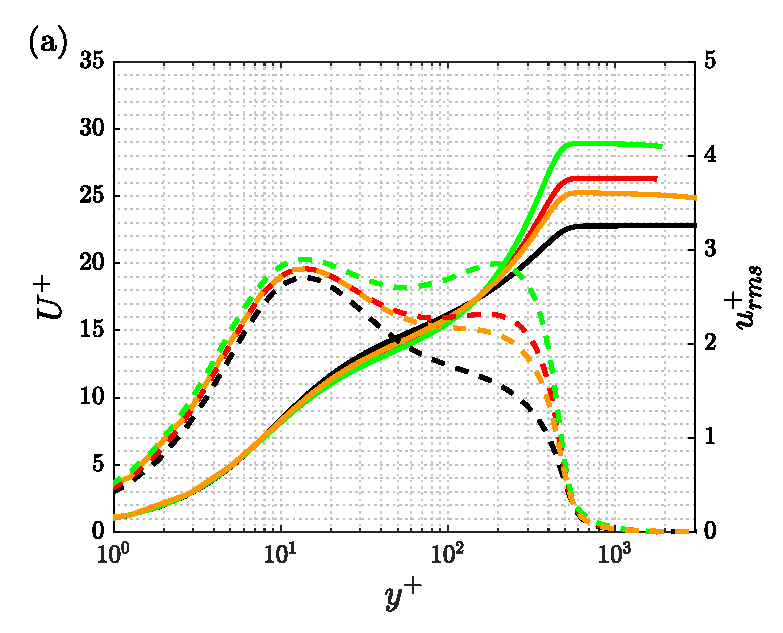
\includegraphics[width=0.49\textwidth]{imgs/stats/U_uu_a.eps}
    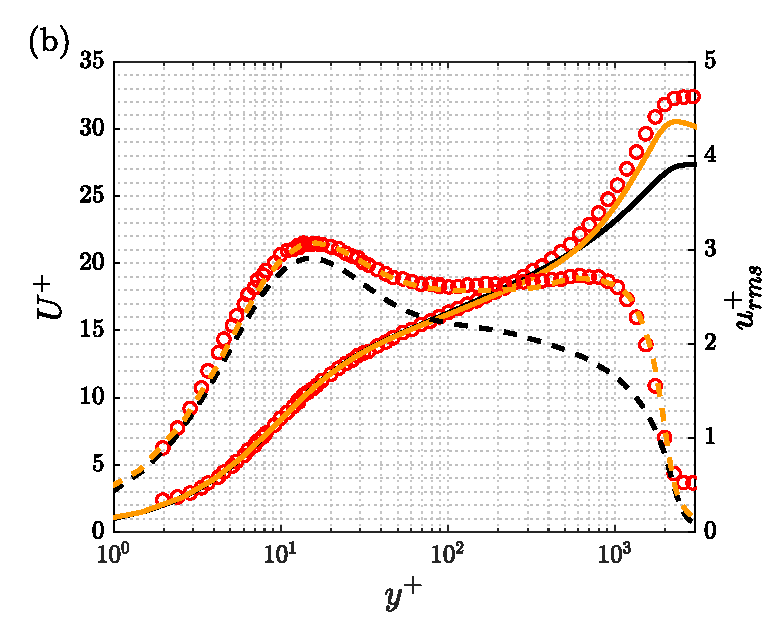
\includegraphics[width=0.49\textwidth]{imgs/stats/U_uu_b.eps}
    \caption{Mean streamwise $U$ (solid lines) and streamwise root mean square $u_{rms}$ or strandard deviation of the streamwise velocity (dashed lines). Wall-normal profiles taken at: (a) $\Rey_{\tau}=500$, (b) $\Rey_{\tau}=2100$. }
    \label{fig:U_uu_cap2}
\end{figure}

\subsection{Friction at the wall, on the friction coefficient $c_f$}

The drag in aerodynamic structures has an important contribution from the friction at the wall, also known as skin friction which is the mean shear stress produced at the wall $\tau_w$, due to the viscous forces.
Instead of $\tau_w$, it is common to look at the friction factor $c_f$ which is a ratio between the friction stresses and the free flow,
\begin{equation}
    c_f = \frac{\rho \tau_w}{1/2 \rho U_e^2} = \frac{2 u_{\tau}^2}{U_e^2} = 2\left( \frac{u_{\tau}}{U_e} \right)^2
\end{equation}
but it can also be seen as an indicator of the friction-velocity with respect to the free-flow velocity.

\begin{figure}
    \centering
    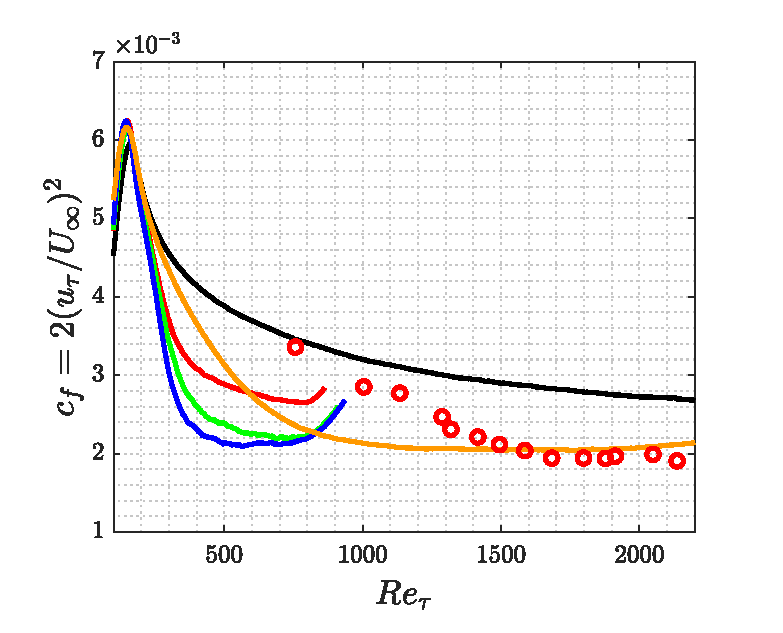
\includegraphics[width=0.85\textwidth]{imgs/stats/cf_Retau.eps}
    \caption{Evolution of the mean friction coefficient $c_f = \pdv{2\overline{\tau_w}}/{U_e^2}$ for ZPG and APG simulations (solid lines) and experiments by \cite{MTL_expSANMIGUEL} (red circles).}
    \label{fig:cap3_evol_cf}
\end{figure}

In Fig.~\ref{fig:cap3_evol_cf} we show the mean friction factor development along the turbulent boundary layers for ZPG and APG simulations and an experimental APG.
It can be seen how for attached flows and near-equilibrium TBLs the trend is positive, decays with the Reynolds number and the value is lower the stronger the APG intensity.
The simulations show an increase for the larger $\Rey_{\tau}$ where the fringe region starts to affect the flow, and this region is not included in the region of interest (ROI) of our database.

The effects of APG on the coefficient $c_f$ are studied through the Renard--Deck (RD) \citep{Renard2016} identity in \textbf{Paper 3} and the Fukagata, Iwamoto \& Kasagi identity (FIK)  \citep{Fukagata2002} in \textbf{Paper 4}.

The FIK decomposition of $c_f$ is adapted to include a join contribution of the pressure gradient and the streamwise convection, looking for a dynamic pressure perspective, instead of treating this antagonizing contributions as a separate entity.

A different approach onto the $c_f$ is that of the RD decomposition, taken from a perspective based on the mean streamwise kinetic energy budget. 
The main contributions to the total $c_f$ are divided in three main terms representing the viscous dissipation, the turbulent kinetic energy production and the spatial growth.
The contribution from the viscous diffusion is mainly located in the inner/near-wall region of the TBL and the influence diminish for stronger APGs, since the influence of the larger scales located in the outer region of the TBL are more energized and its effects on $c_f$ are larger.
The TKE Production close to the wall have a near-wall peak that influences $c_f$, but the influence of APGs produce a strong outer-peak in the outer region.
The spatial growth contribution is further decomposed into three subterms, the main ones are due to the mean convection $\Vec{U}\cdot \nabla\Vec{U}$ (which has a positive contribution across the TBL) and a direct contribution of the pressure-gradient (which has a negative contribution on $c_f$). These terms are more relevant the stronger the APG is and decrease with $\Rey$, and their influence is mostly located in the outer/wake region of the TBL.


\section{Spectral decomposition}
To have a better understanding on the perturbations we can use some mathematical tools such as the decomposition of the spatial-temporal signal using correlations, orthogonal modes, coherent structures, etc.
The use of orthogonal modes allows to decompose the energy of the perturbations into each mode in an unique way, so the sum of the energy contained in all the modes is equivalent to the total energy of the perturbations. 

In signal analysis an orthogonal decomposition which is commonly used is the Fourier decomposition which enables to look for phenomena that repeats with a certain time or spatial frequency. The energy or power associated with each mode is called energy spectra (if the signal is finite such as pulses) or power spectra (if the signal is such as sinusoidal waves, whose domain and energy is not finite, however its power is). Remember that the power is the ratio of the energy over time, where the time goes to infinity (in the case of using temporal series).
Since we are dealing with signals which are periodic in the homogeneous dimension $z$ and are not limited in time, we will use the terminology of power spectra (PS) instead of energy spectra. 
The modes in $z$ have a wavenumber $k_z$ and a wavelength $\lambda_z=2\pi/L_z$ where $L_z$ is the spanwise period of the domain. The same analysis can be applied in time, where we will use $k_t$ and $\lambda_t$.
For a signal $x(t)$, with $X(k_t)$ being its Fourier transform, the power of each mode is $|X(k_z)|^2$, the squared amplitude of the mode. For a perturbation velocity, the power can be calculated as,
\begin{equation}
    PS_{u_i\myprime u_j\myprime}(k_z) = \mathcal{F}(u_i \myprime)  \mathcal{F}^*(u_j \myprime),
    \label{eq:power_sp}
\end{equation}
where $\mathcal{F}()$ is the Fourier transform and $\mathcal{F}^*()$ represents the complex conjugate and the definition has been expanded to include the power spectra of the quantity $\langle u_i\myprime u_j\myprime \rangle_{z}$, also known as cospectra.
Using the properties of the Fourier transform, the multiplication in Fourier space represented in Eq.~\ref{eq:power_sp} represents the Fourier transform of the two-point correlation function $\mathcal{R}_{u_i\myprime, u_j\myprime}(\delta z)=u_i\myprime \star u_j\myprime$, where $\delta z$ is the lag or distance between the two points where we look for the correlation of their velocity perturbations. According to the Wiener--Khinchin theorem, we can calculate the PS through as the Fourier transform of $\mathcal{R}_{u_i\myprime, u_j\myprime}$ or from the power spectra throught the inverse Fourier transform $\mathcal{F}^{-1}()$ we can obtain the two-point correlation function.

Note that for velocity perturbations, since Fourier modes are orthogonal, the sum of the PS for all the modes is equal to the averaged Reynolds stress,
\begin{equation}
    \langle u_i\myprime u_j\myprime \rangle_{z} = \sum_{k_z} PS_{u_i\myprime u_j\myprime}(k_z)
\end{equation}

This step can be performed for each time step and averaged over time to obtain $\langle\langle u_i\myprime u_j\myprime \rangle_{z}\rangle_{t} = \overline{u_i\myprime u_j\myprime}$ or it can also be the result of a 2D spectral decomposition in both time and $z$, where the sum extends to all the spatial and temporal modes.

The PS is useful for discrete systems, and it is the first step when we calculate numerically the spectra of a the Reynolds-stresses. It is also interesting to see how the power spectra is distributed along the wavenumbers or the wavelengths, obtaining a power spectral density (PSD).
The average in time of the PSD in wavenumbers is $\phi_{u_i\myprime u_j\myprime}=\langle PS \rangle_t/\mathrm{d} k_z$ while the average in time PSD in wavelengths is $\psi_{u_i\myprime u_j\myprime}= \langle PS \rangle_t/\mathrm{d} \lambda_z$. Both densities can be linked using $\mathrm{d}(\lambda_z) = \mathrm{d}(2\pi/k_z) = -2\pi\mathrm{d}k_z/k_z^2$:

\begin{equation}
    \psi_{u_i\myprime u_j\myprime} = 
    \frac{ \langle PS_{u_i\myprime u_j\myprime} \rangle_t}{\mathrm{d} \lambda_z} =
    -\frac{ \langle PS_{u_i\myprime u_j\myprime} \rangle_t}{\mathrm{d} k_z} \frac{k_z^2}{2\pi},
\end{equation}
where the minus sign is taking care by inverting the limits of integration to obtain the total RS (small to large wavenumbers is equivalent to integrate from large to small wavelengths).

\begin{equation}
\label{eq:sum_ps}
    \overline{u_i\myprime u_j\myprime} = 
    \int_{k_z=k_0}^{k_z=k_{N}}   \phi_{u_i\myprime u_j\myprime}  ~ \mathrm{d} k_z =
    \int^{\lambda_z = 2\pi/k_0}_{\lambda_z = 2\pi/k_{N}}  \psi_{u_i\myprime u_j\myprime}  ~ \mathrm{d} \lambda_z
\end{equation}

In Fig.~\ref{fig:PS_PSD} we show for a ZPG TBL, different representations of the PSD of $\overline{u\myprime u\myprime}$ where the image with the black contours represent a streamwise profile at $\Rey_{\tau}=2000$ while the red contours are taken at a position where $\Rey_{\tau}=500$.

\begin{figure}[h!]
\centering
% \captionsetup{width=0.99 \textwidth}
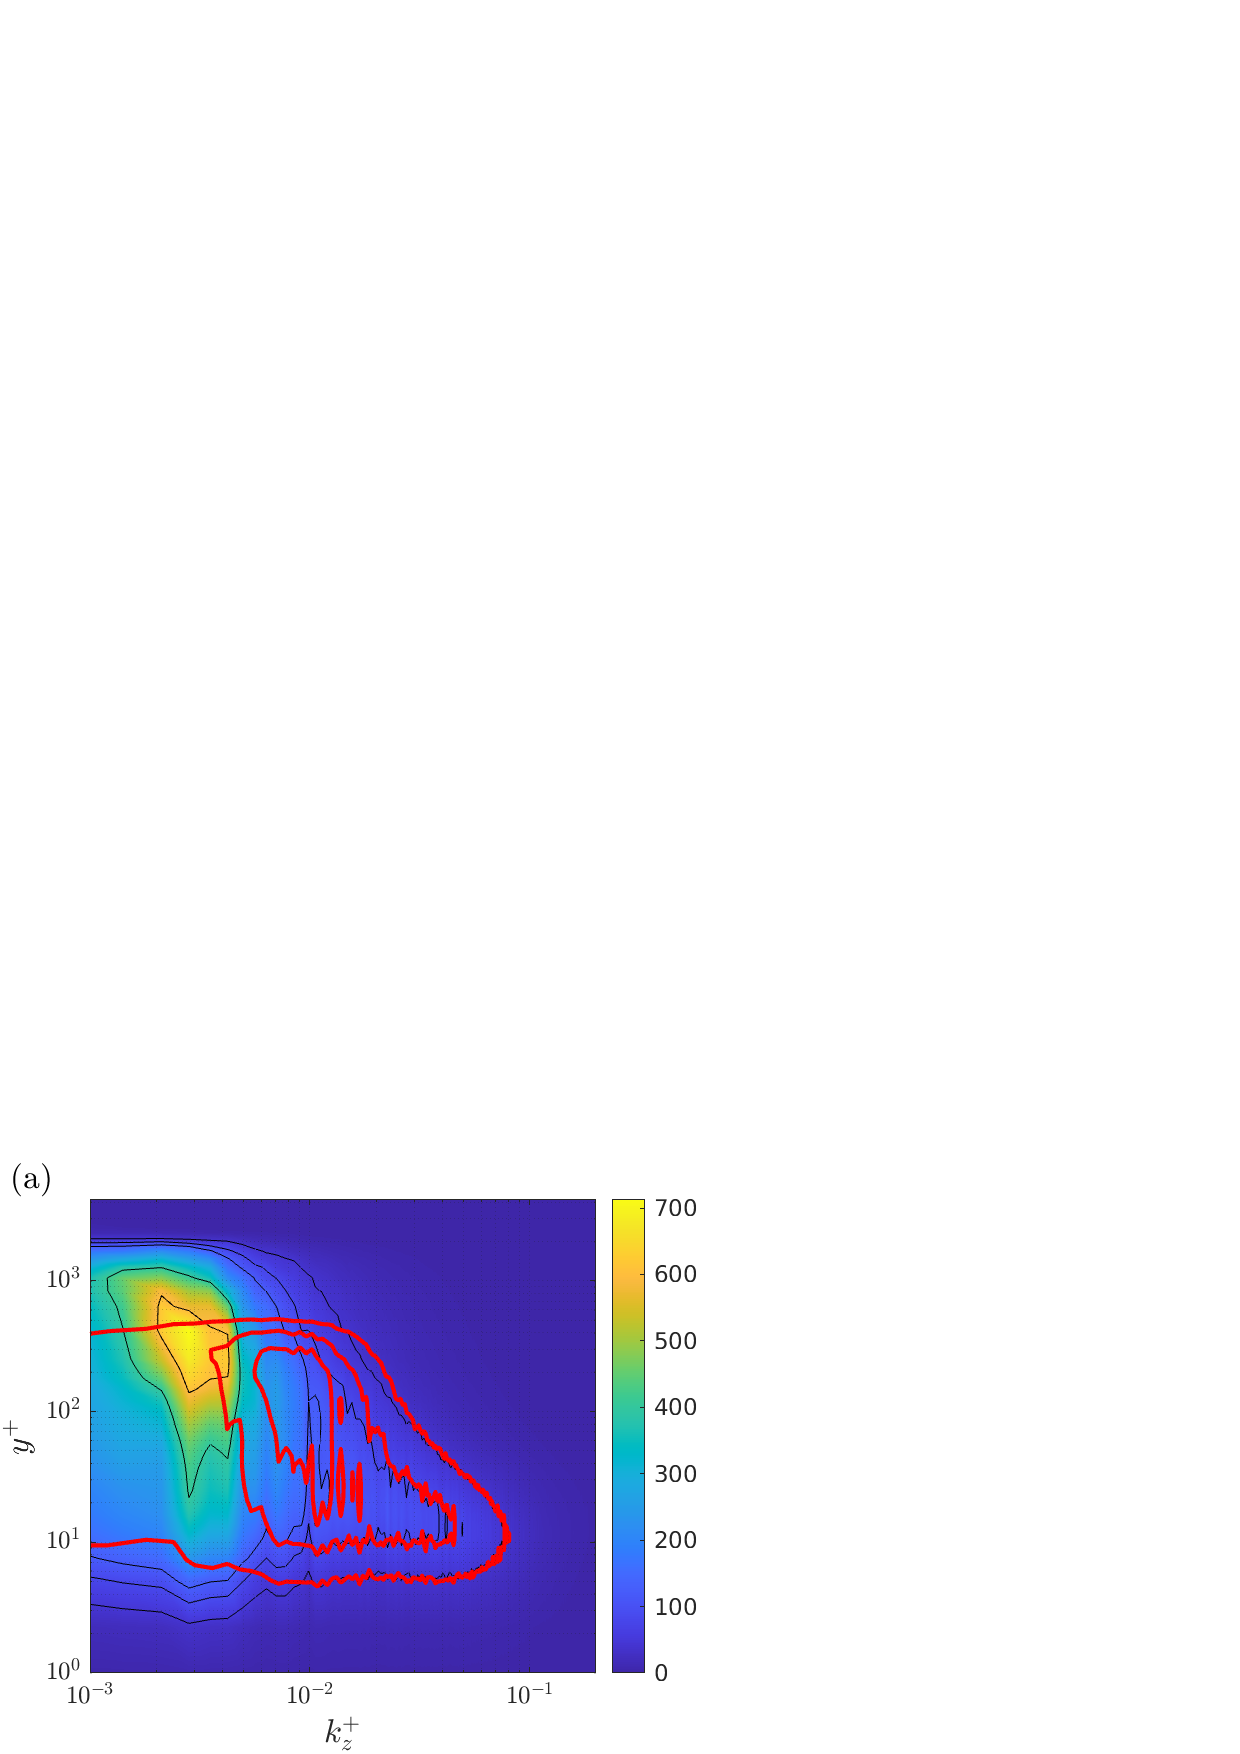
\includegraphics[width=0.32\textwidth ]{imgs/spec/ZPG_Ret_500_2000_PSdkz_kz_ltau_y_ltau.jpg}
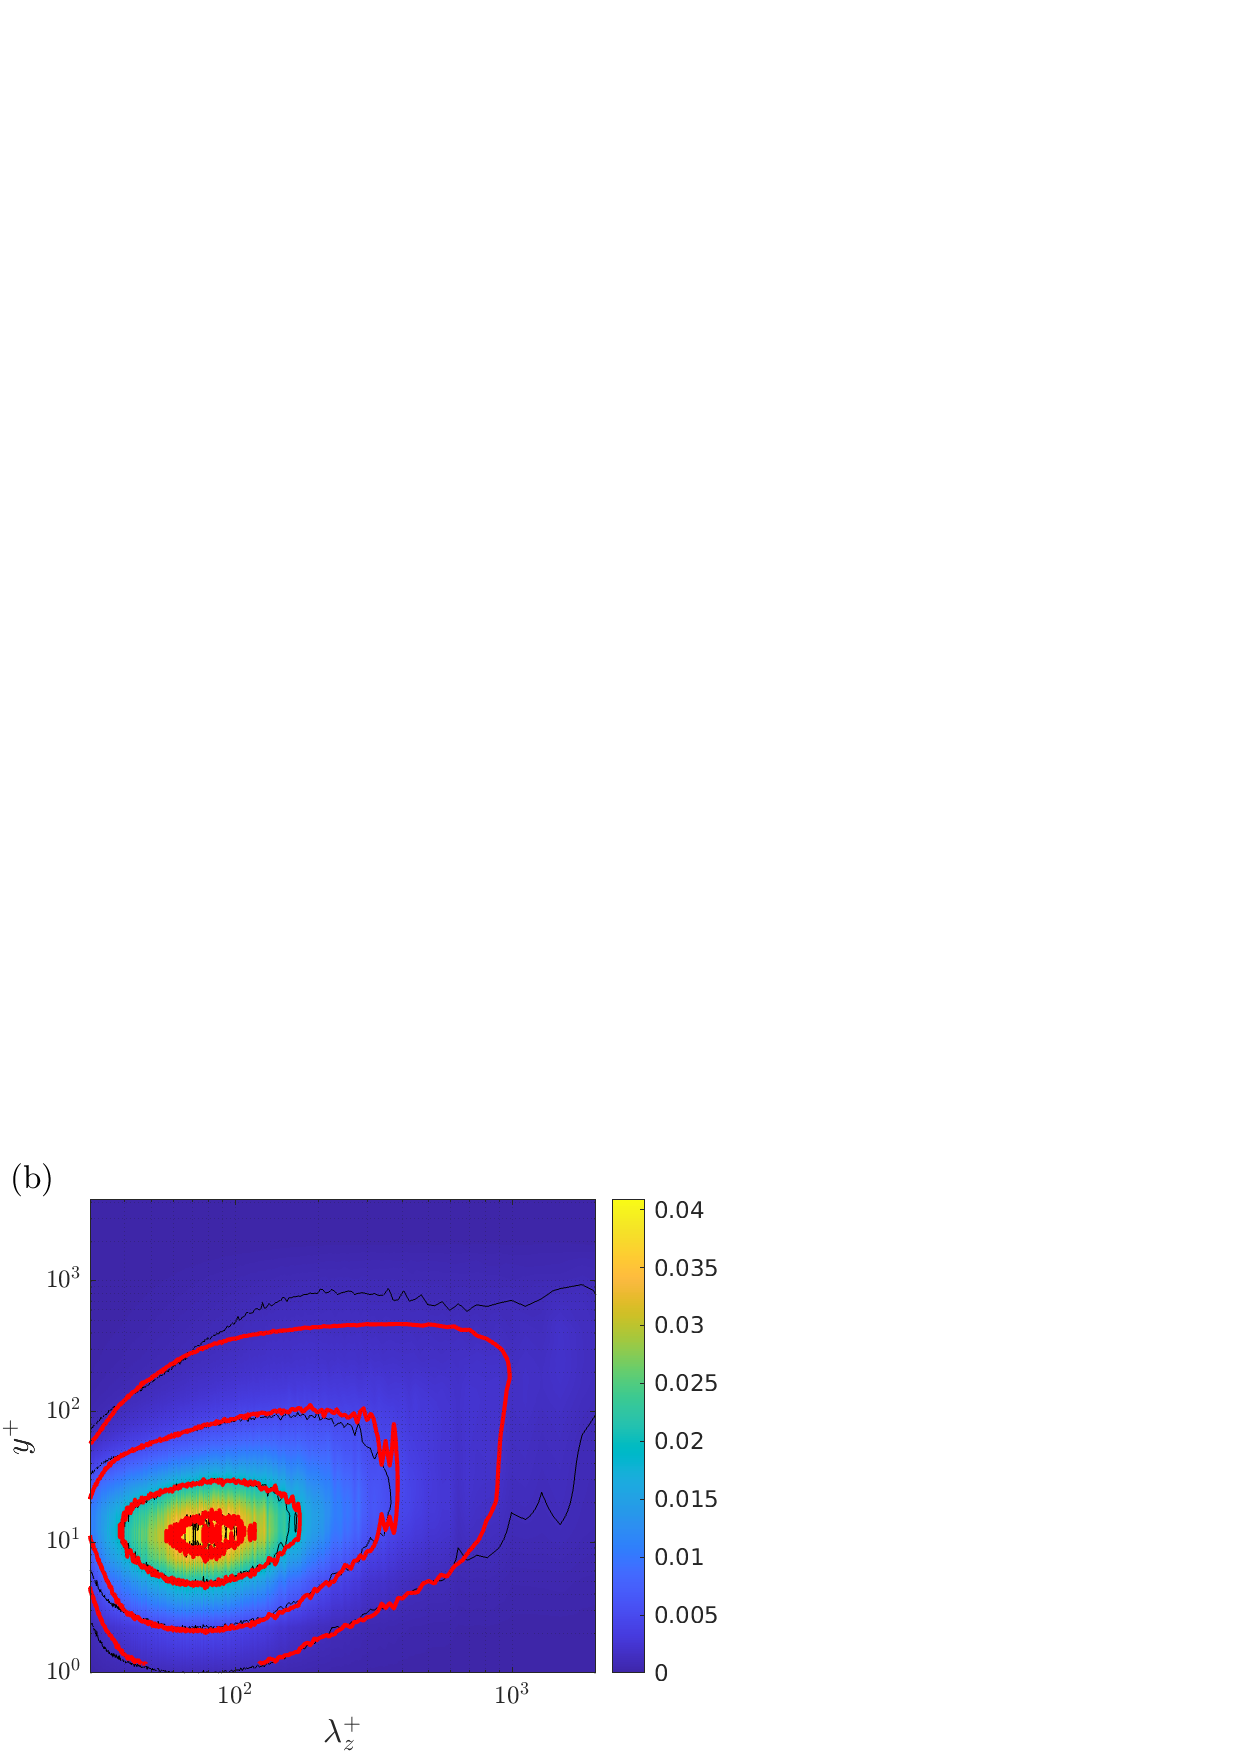
\includegraphics[width=0.32\textwidth]{imgs/spec/ZPG_Ret_500_2000_PSdlambdaz_lambdaz_ltau_y_ltau.jpg}
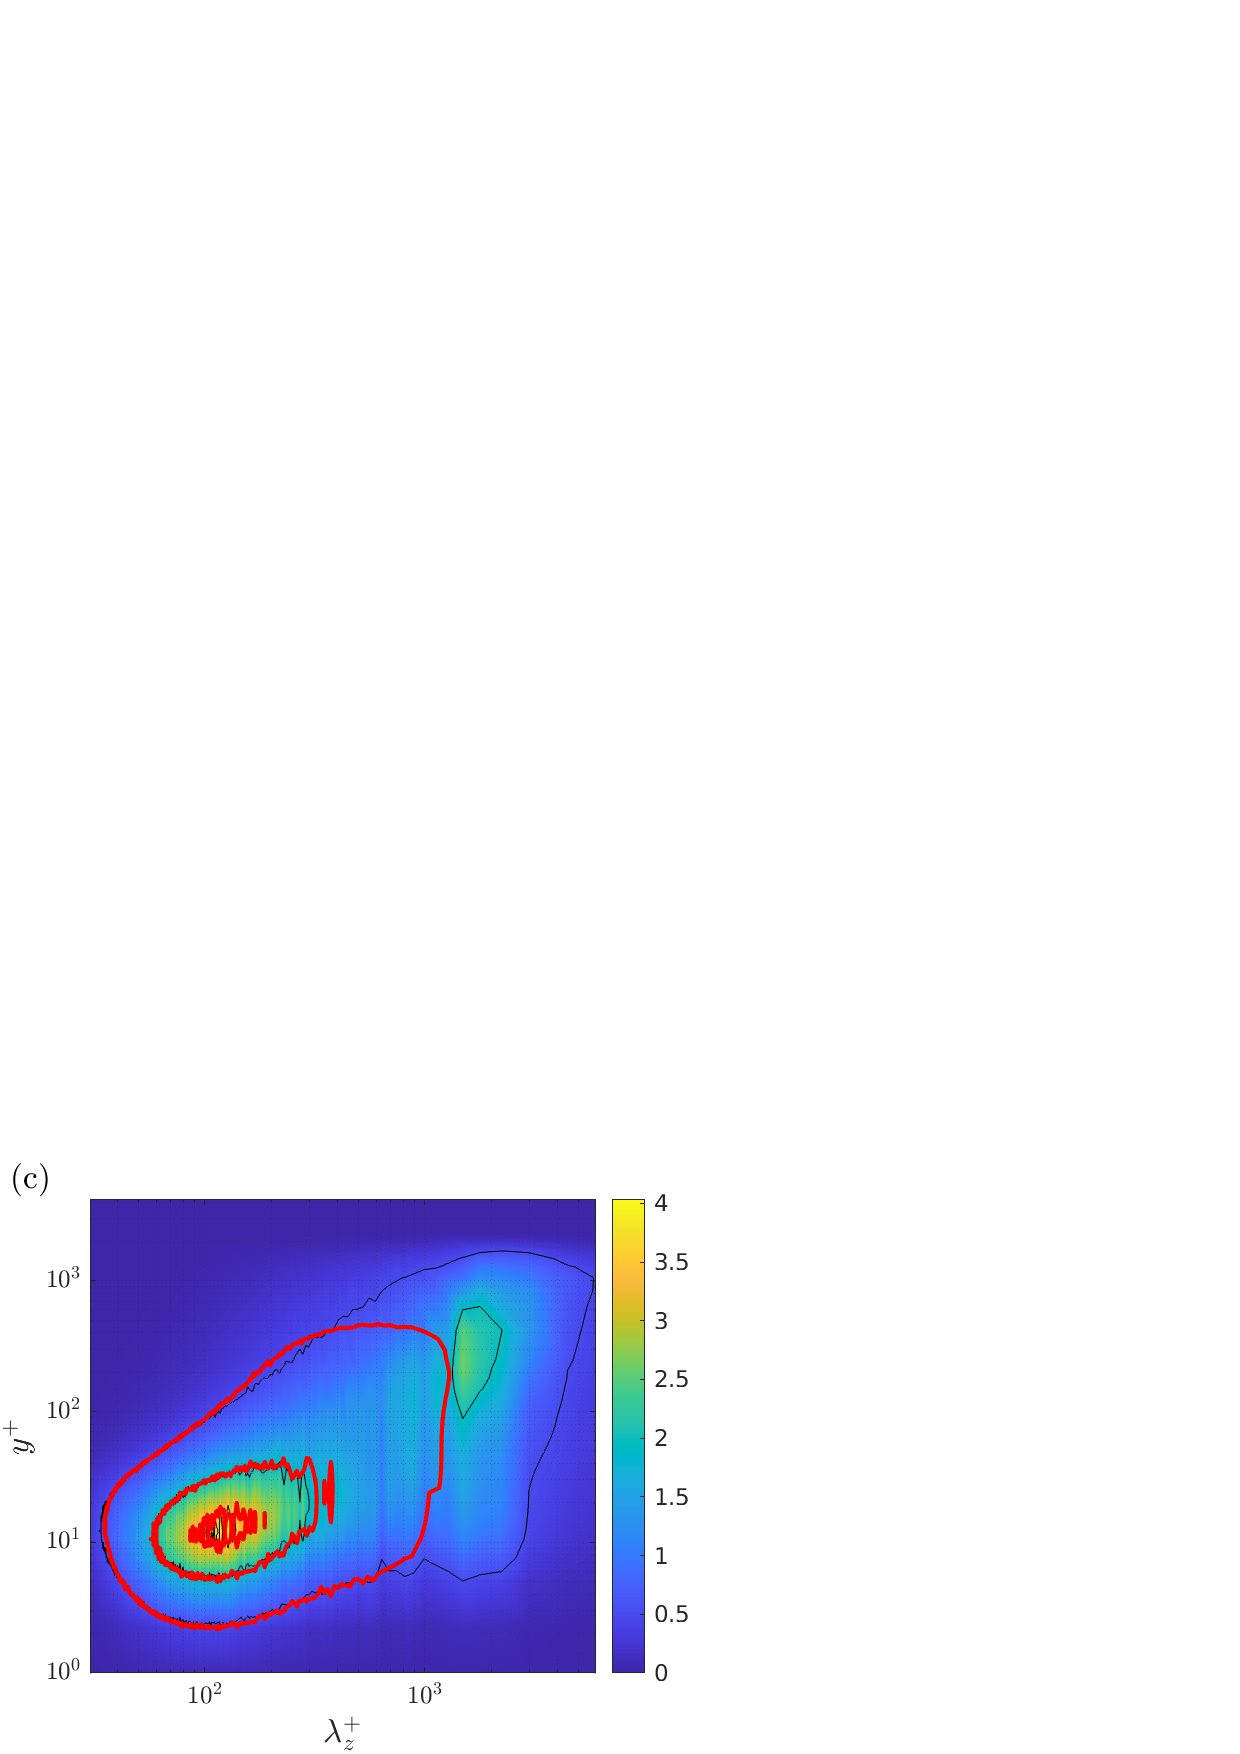
\includegraphics[width=0.32\textwidth]{imgs/spec/ZPG_Ret_500_2000_kPSdkz_lambdaz_ltau_y_ltau.jpg}
\caption{ \label{fig:PS_PSD} Spanwise spectra of the streamwise Reynolds stress $\overline{uu}(y)$. (a) Power spectral density $\phi_{u\myprime u\myprime}(y,k_z)$; (b) Power spectral density $\psi_{u\myprime u\myprime}(y,\lambda_z)$; (c) premultiplied power spectral density $k_z\phi_{u\myprime u\myprime}$. Wavenumbers, wavelengths, wall-normal position and power spectra scaled in viscous units.}
\end{figure}
% contours: Retau 2000: [40 80  120 400 600]; [0.001 0.005 0.02 0.035 0.04] ;  [ 0.5 2 3.5]; 
% contours: Retau  500: [40 80  120        ]; [0.001 0.005 0.02 0.035 0.04] ;  [ 0.5 2 3.5]; 

The PS and the PSD in the wavenumbers $\phi_{u\myprime u\myprime}(y,k_z)$ present the same features as in Fig.~\ref{fig:PS_PSD}(a), since $dk_z$ or $dk_z^+$ are constant factors that does not vary with the wavenumbers. It shows a high content of power/energy of structures with a very low wavenumber which are very wide. It is possible to see similarities in the contours at different Reynolds numbers (red and black lines) in the region of high wavenumbers (small scales), although the energetic level is very low compared to that of the low wavenumbers (large scales).
The PSD in wavelengths $\phi_{u\myprime u\myprime}(y,\lambda_z)$ is represented in Fig.~\ref{fig:PS_PSD}(b) and it focuses on the small scales. It shows that the density of power/energy in the small scales (short wavelengths) is very similar at different Reynolds numbers and larger than the PSD of the wider scales (large $\lambda_z^+$). 
From Fig.~\ref{fig:PS_PSD}(a) and (b) we see that the small scales have a small content of the total RS energy, but their small size make the density in waveleghts to be very concentrated, while for the wider scales is the opposite, the energy they contain is very large, but their big size make the PSD to be very low or disperse.
If we write both PSD as a function of $\phi_{u\myprime u\myprime}$, in Fig.~\ref{fig:PS_PSD}(a) we show $\phi_{u\myprime u\myprime}$ while in Fig.~\ref{fig:PS_PSD}(b) it would be $k_z^2 \phi_{u\myprime u\myprime}$, the premultiplication factor $k_z^2$ is responsible to augment the effects of the small scales while diminishing the effects of the large scales. Fig.~\ref{fig:PS_PSD}(c) shows $k_z \phi_{u\myprime u\myprime}$, whose effect equilibrates the effect of the large and small scales obtaining a better visualization of both scales.

The premultiplied PSD $k_z \phi_{u\myprime u\myprime}$ is widely used and it has a geometrical explanation.
Since the range of energetic scales is so large that we observe very small scales close to the wall and very large scales of the size of $\delta_99$, the use of logarithmic axis helps to expand the region of small $\lambda_z$ and the region close to the wall.
If we use logarithms in the definition of wavelength, $ \mathrm{ln}(\lambda_s) = \mathrm{ln}(2\pi) - \mathrm{ln}(k_z)$, and apply the differential, $\mathrm{d}(\mathrm{ln} \lambda_z) = -\mathrm{d}(\mathrm{ln} k_z)$, and together with $\mathrm{d}k_z = k_z \mathrm{d}(\mathrm{ln} k_z)$ can be substituted in Eq.~\ref{eq:sum_ps} to obtain:
\begin{equation}
    \overline{u_i\myprime u_j\myprime} = 
    \int_{k_0}^{k_{N}}   \phi_{u_i\myprime u_j\myprime}  ~ \mathrm{d} k_z = 
    \int_{k_0}^{k_{N}}   \phi_{u_i\myprime u_j\myprime} k_z  ~ \mathrm{d}( \mathrm{ln} k_z) = 
    \int^{\lambda_0}_{\lambda_{N}}   \phi_{u_i\myprime u_j\myprime} k_z ~ \mathrm{d}( \mathrm{ln} \lambda_z).
\end{equation}

The premultiplication by $k_z$ can be seen here as a factor to visualize a corrected area after scaling the axis with a logarithmic scale.
From here on the PSD will always be represented in its premultiplied form $k_z\phi$ to have a clear visualization of the effects of large and small scales at the same time.

\subsection{Wide scales in turbulence. Channel Flows}
It has been seen that the big scales contains a large part of the turbulent energy, although the density spectral density is low.
When we model the turbulent flow, the size of the domain imposes a limit on the size of the scales that can be simulated. In a periodic domain, the largest scale corresponds to $L_x$ and the wider scale to $L_z$. Bigger scales will be seen as infinit in size because of the periodicity, and the spectral energy will be stored in the zero-wavenumbers.

The energy contained in the zero-wavenumbers is affected by the averaging.

If the size of the domain is not large or wide enough, the bigger turbulent scales will not be able to be captured and the energetic spectrum will not be correct, affecting the total statistics such as the Reynolds stresses and the mean velocity profiles.
Many analysis on the size of the domain has been performed on canonical turbulent channel flows for it simplicity.
\highlight{Minimal channels are those small domains that assure }
On the other way, the largest scales in channel flows where looked for in \highlight{CITAR ADRIAN que descubrieron bla bla}.
The study on the wider scales was based on two-point correlations, but no other study similar to \highlight{CITAR ADRIAN} was performed in the spanwise direction.

To have a better understunding of the wide scales obtained in APG TBLs and the effects of the domain size, we decided to study first the effect on wide-channels.
Three simulations were performed of turbulent channel flows at $\Rey_{\tau} = 550 $ under similar conditions, with the only excemption the width of their domains which was doubled from one channel to another as it can be seen in Tab.~\ref{tab:param_WC_cap2}.
 
\begin{table}
    \begin{center}
    \def~{\hphantom{0}}
    \begin{tabular}{ l r  r  r  r }
    Case  & $L_x/h$ & $L_y/h$ & $L_z/h$ &  Colour     \\[3pt]
    C1    & 8$\pi$  &    2    & 4$\pi$  &  \redline   \\
    C2    & 8$\pi$  &    2    & 8$\pi$  &  \redline   \\
    C3    & 8$\pi$  &    2    & 16$\pi$ &  \redline   \\
    \end{tabular}
    \caption{Parameters of the channel flows simulations. The reference length $h$ corresponds to half the channel's height. The box size is $(L_x/h, L_y/h , L_z/h)$.}
    \label{tab:param_WC_cap2}
    \end{center}
\end{table}

\highlight{The contours of the PS or the spectral density $\phi(k_Z, y)$ are not closed for the largest scales when $k_z \rightarrow 0$. The largest scale captured by Fourier analysis corresponds to $k_Z=(2\pi)/L_z$ or $L_z$, and $k_z=0$ corresponds to an averaged energy. 
The property where the integral of the PSD equals the RS component includes the energy contained in the wavenumber $k_z=0$. The premultiplication by $k_z$ automatically cancels that energy, making it inappropriate to use premultiplied spectra for integral analysis. 
Then this question arises, ``is it possible to have a domain $L_z$ where the largest Fourier scales $\lambda_z=\{L_z, L_z/2, ... \}$ does not contain spectral energy, therefore the contours are closed?''.
And the answer is that it depends on the averaging that we use. This answer will be explained using the Reynolds-average decomposition that we have introduced previously, and apply it to the component $u$.}
With $PS_T$ we denote the power spectra of the total velocity $u$, and the energy contained in the wavenumber $k_z$ corresponds to the average in $z$.


\begin{equation}
    PS_T = \mathcal{F}(u)\mathcal{F}^*(u) = \mathcal{F}(U)\mathcal{F}^*(U) + \mathcal{F}(u\myprime)\mathcal{F}^*(u\myprime) + \mathcal{F}(U)\mathcal{F}^*(u\myprime) + \mathcal{F}(u\myprime)\mathcal{F}^*(U)  
\end{equation}

\begin{flalign}
    % \label{eq:intsc_3term_small}
     PS_T =& \mathcal{F}(u)\mathcal{F}^*(u) &&\\\nonumber
     =&  \mathcal{F}(U)\mathcal{F}^*(U) + \mathcal{F}(u\myprime)\mathcal{F}^*(u\myprime) + \mathcal{F}(U)\mathcal{F}^*(u\myprime) + \mathcal{F}(u\myprime)\mathcal{F}^*(U) &&\\\nonumber
     =&  UU + \mathcal{F}(u\myprime)\mathcal{F}^*(u\myprime) + U(\mathcal{F}(u\myprime) + \mathcal{F}^*(u\myprime)) &&\\\nonumber
\end{flalign}  
\rev{and the last term vanishes when the time average is performed?}

\begin{equation}
\begin{split}
    % \label{eq:intsc_3term_small}
     PS(k_z=0,t) = \langle u\myprime \rangle_z \langle u\myprime \rangle_z  (t) \\
     \langle PS(k_z=0) \rangle_t = \langle (\langle u\myprime \rangle_z)^2 \rangle_t > 0,
\end{split}
\end{equation}
since by definition, $U$ and $u\myprime$ are chosen as a constant and a fluctuation based on the total average $\overline{( \cdot )} = \langle \langle ( \cdot ) \rangle_z \rangle_t$, and $\overline{u\myprime}=0$, but $ \langle u\myprime \rangle_z \neq 0$.

Therefore, the energy contained in $k_z=0$ can not be 0, but it is somehow a result of the average used for the decomposition.
What can be study is how the energy contained in $k_z=0$ changes with $L_z$, and even more relevant from the physical point of view is how much is the energy contained in the first wavenumbers or the largest scales $\lambda_z=L_z, L_z/2, L_z/3,...$.


\subsection{Spectral results on APG}

In \textbf{Paper 1} the 1D spanwise spectra and the 2D spanwise and temporal spectra of the APG TBL where shown and compared to those of a ZPG TBL \citep{EAmorZPG}. By using percentage contours it was possible to show a similar behaviour in the mild APG and the ZPG simulations at different Reynolds numbers in the small-scale energy region close to the wall around an spectral near-wall peak or spectral inner peak (sIP) at $y^+\approx 15$ and $\lambda_z^+\approx 120$. Another region with similar shape is in the wake region with an spectral outer peak that seemed to scale with the Reynolds number.
Another region is that of small-scale energy in the wake region, which is only present in the APG simulation and not in the ZPG case.

\begin{figure}[h!]
\centering
% \captionsetup{width=0.99 \textwidth}
\includegraphics[width=0.48\textwidth]{ZPG_uu.jpg}
\includegraphics[width=0.48\textwidth]{APG_uu.jpg}
% 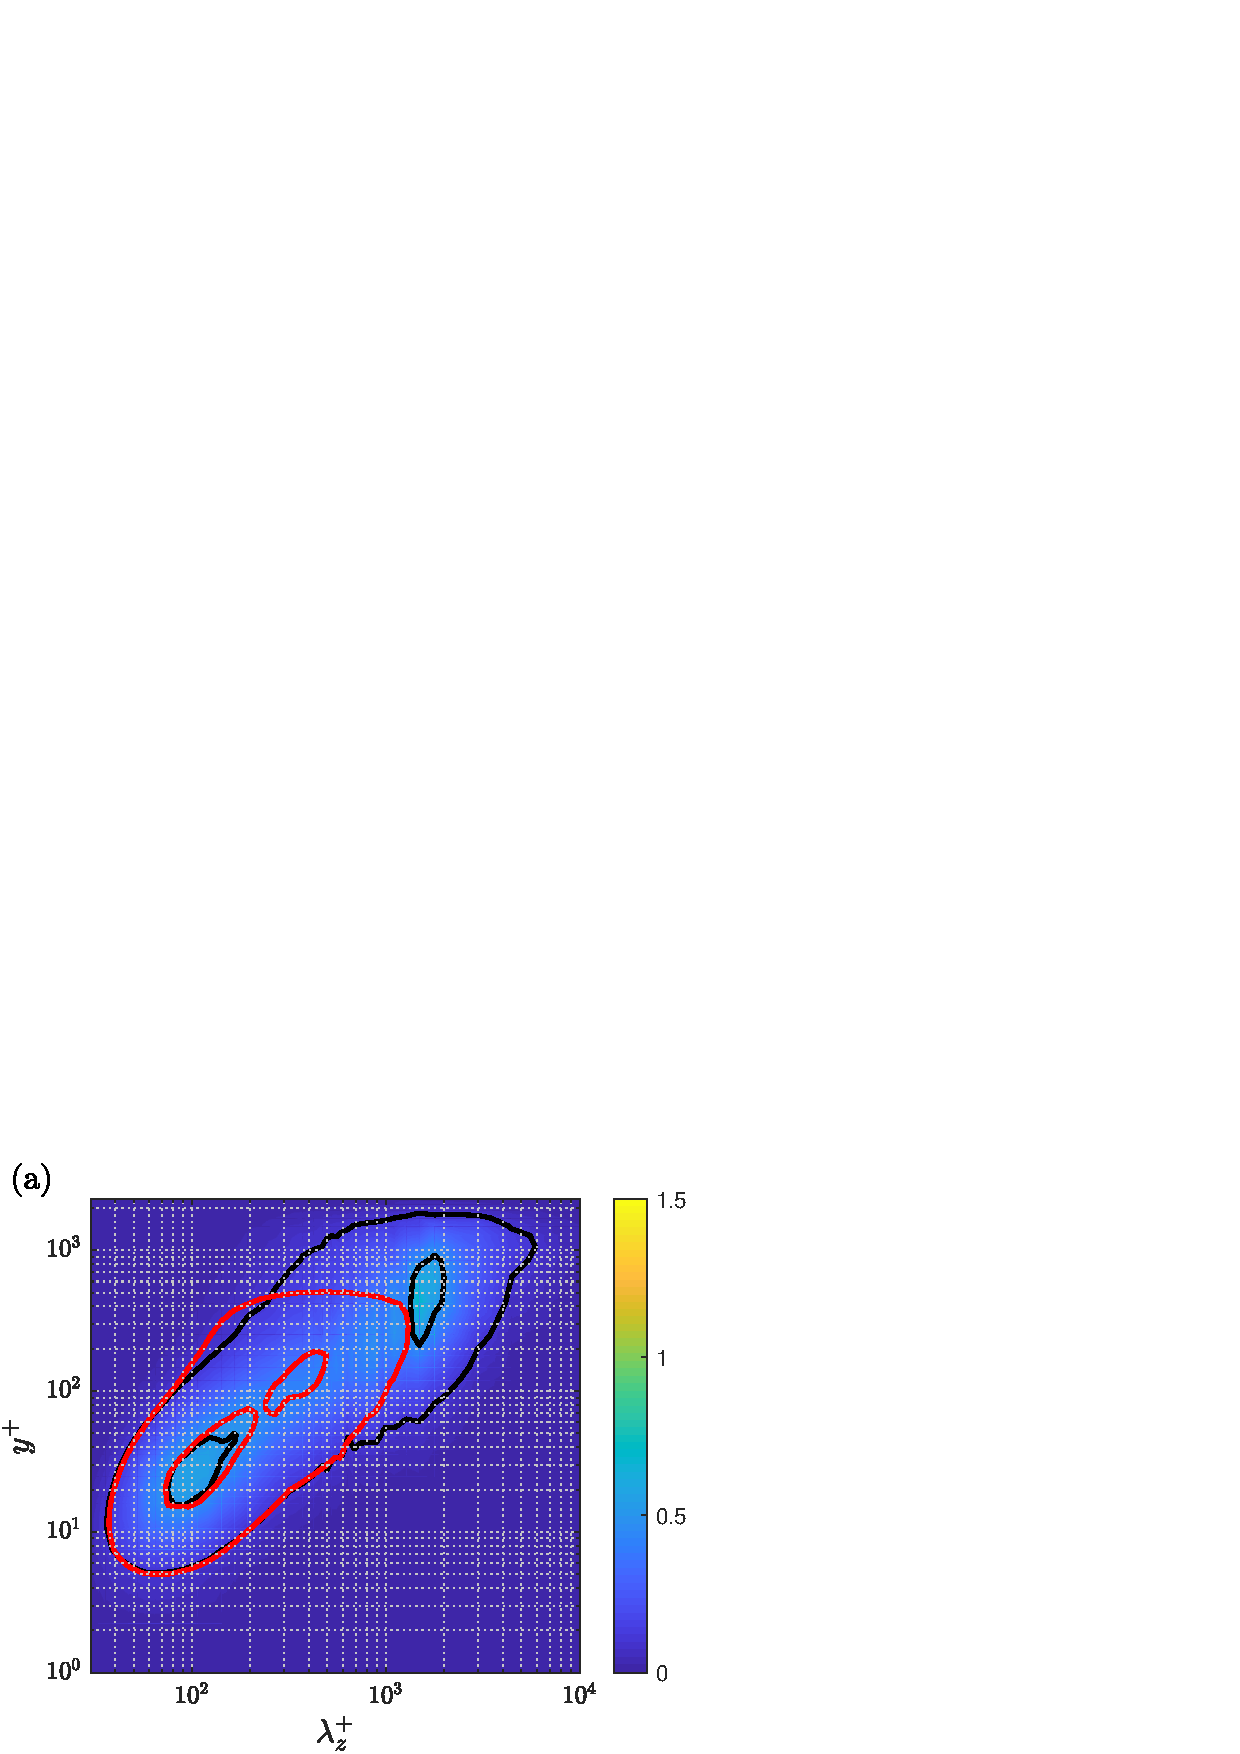
\includegraphics[width=0.48\textwidth]{ZPG_uv.jpg}
% 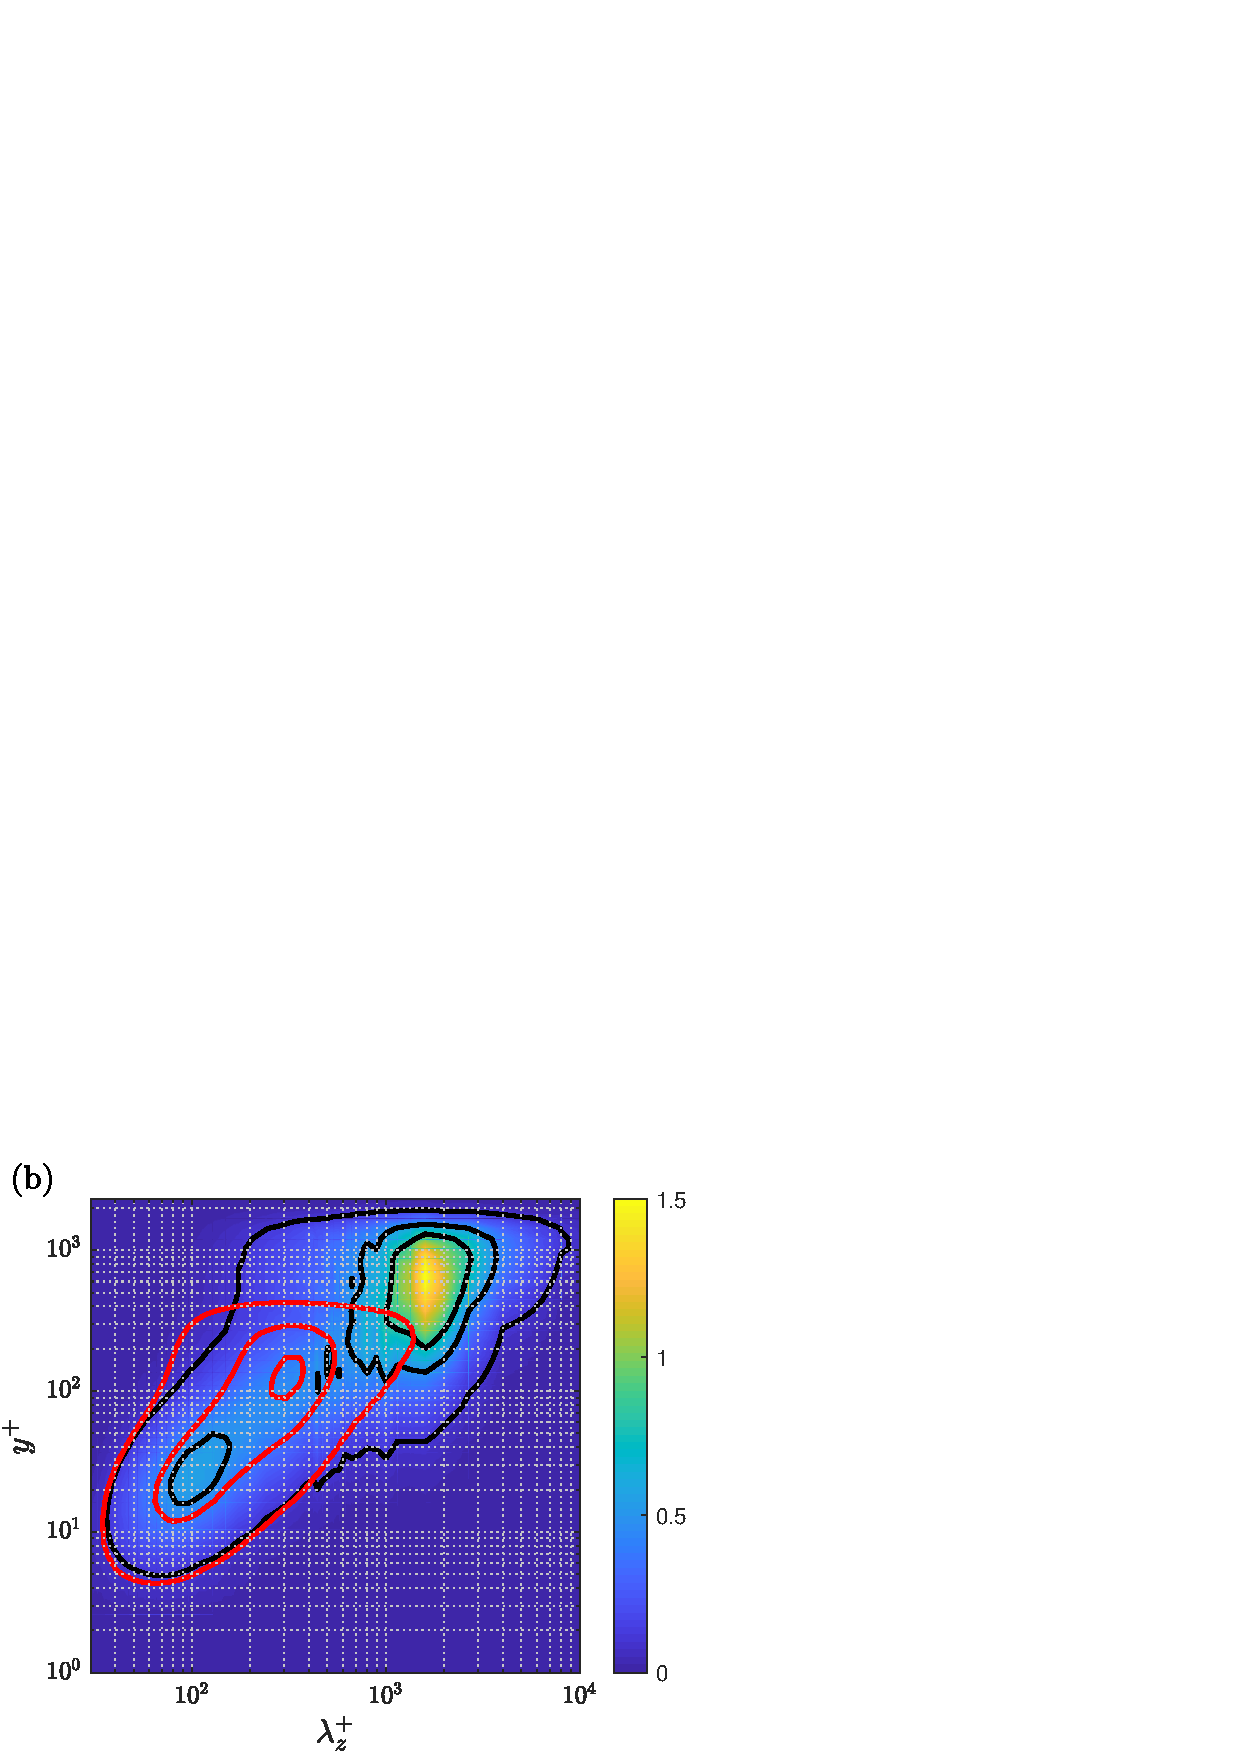
\includegraphics[width=0.48\textwidth]{APG_uv.jpg}
\caption{ \label{fig:ZPG_APG_Ret_500_2000_uu} Premultiplied spectrum $k_z\phi_{uu}$ for (a)ZPG and (b)b1.4 simulations. Red contours at $\Rey_{\tau}=500$ and background and black contour are at a positions $\Rey_{\tau}=2000$. }
\end{figure}

\begin{figure}[h!]
\centering
% \captionsetup{width=0.99 \textwidth}
% \includegraphics[width=0.48\textwidth]{ZPG_uu.jpg}
% \includegraphics[width=0.48\textwidth]{APG_uu.jpg}
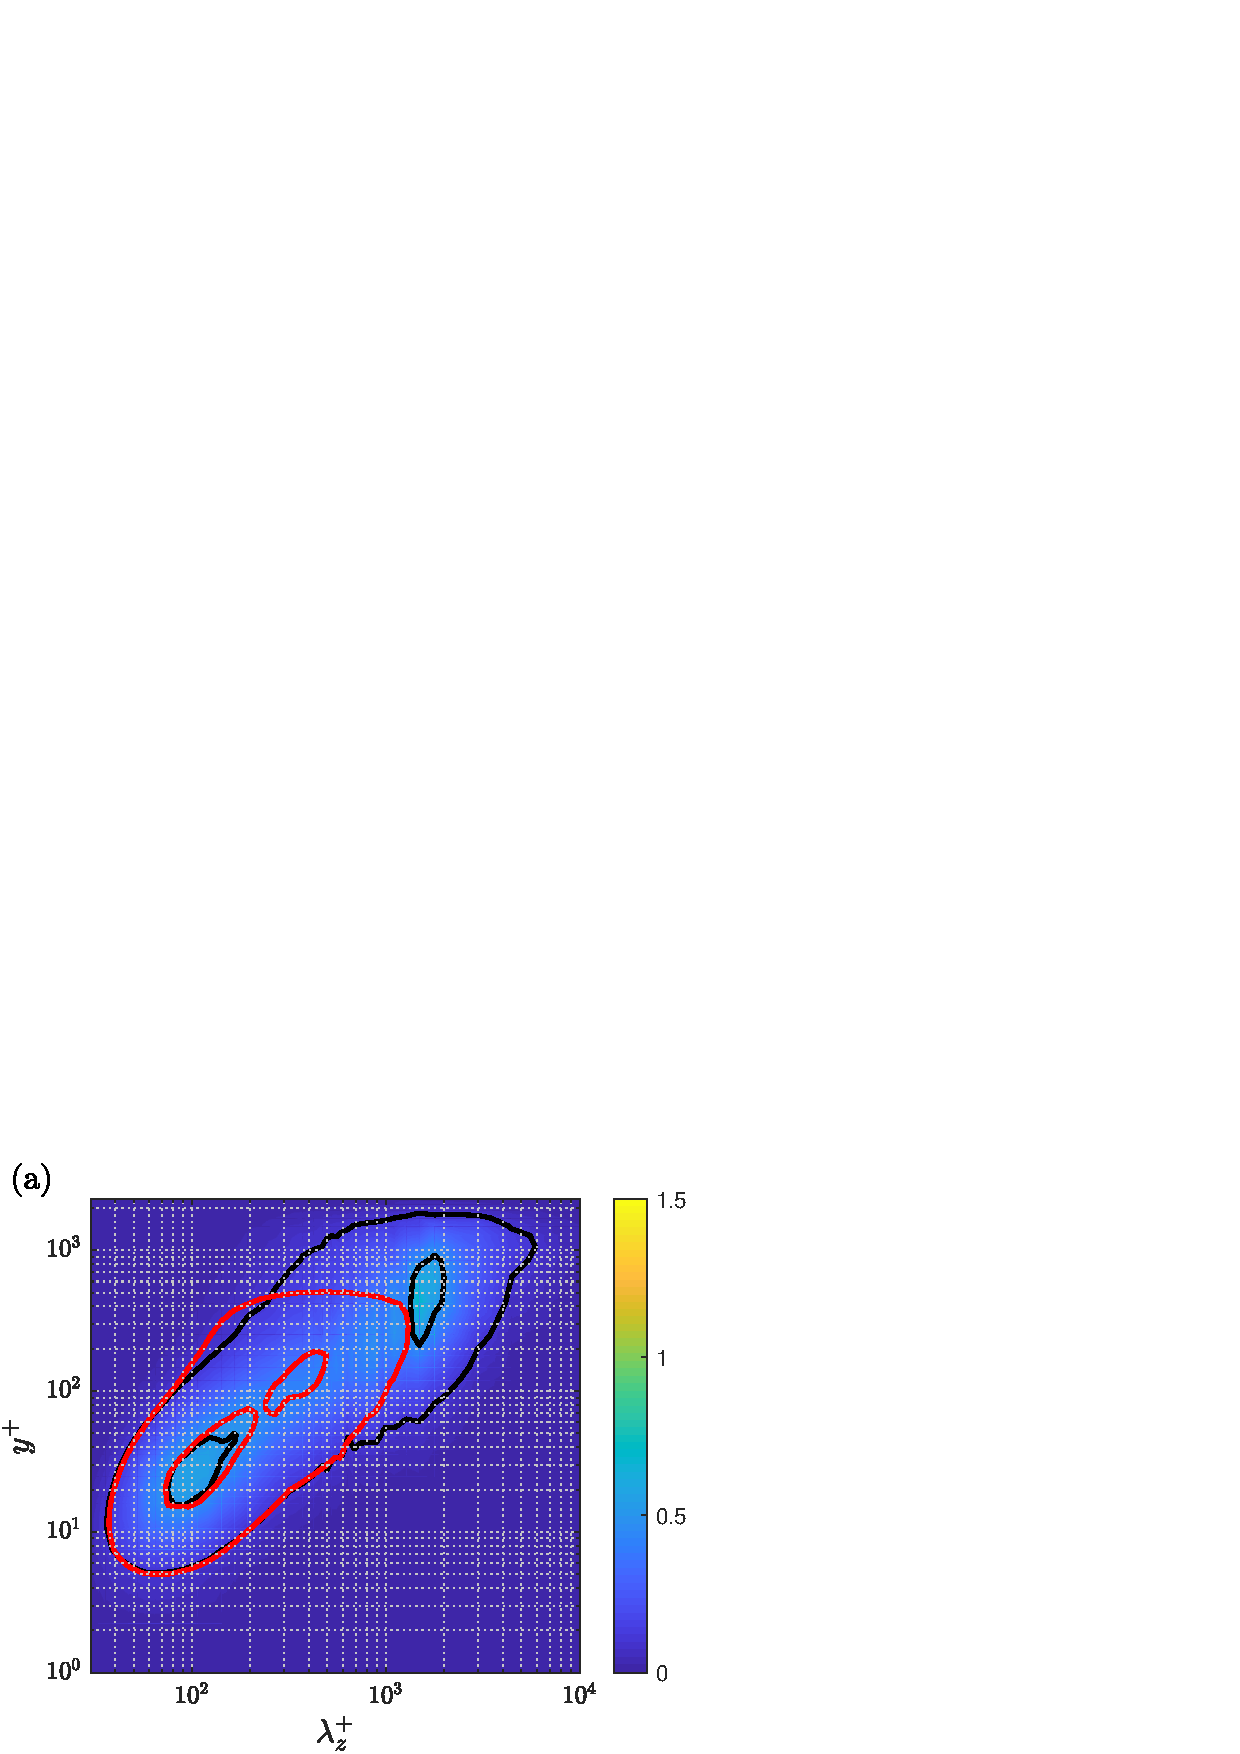
\includegraphics[width=0.48\textwidth]{ZPG_uv.jpg}
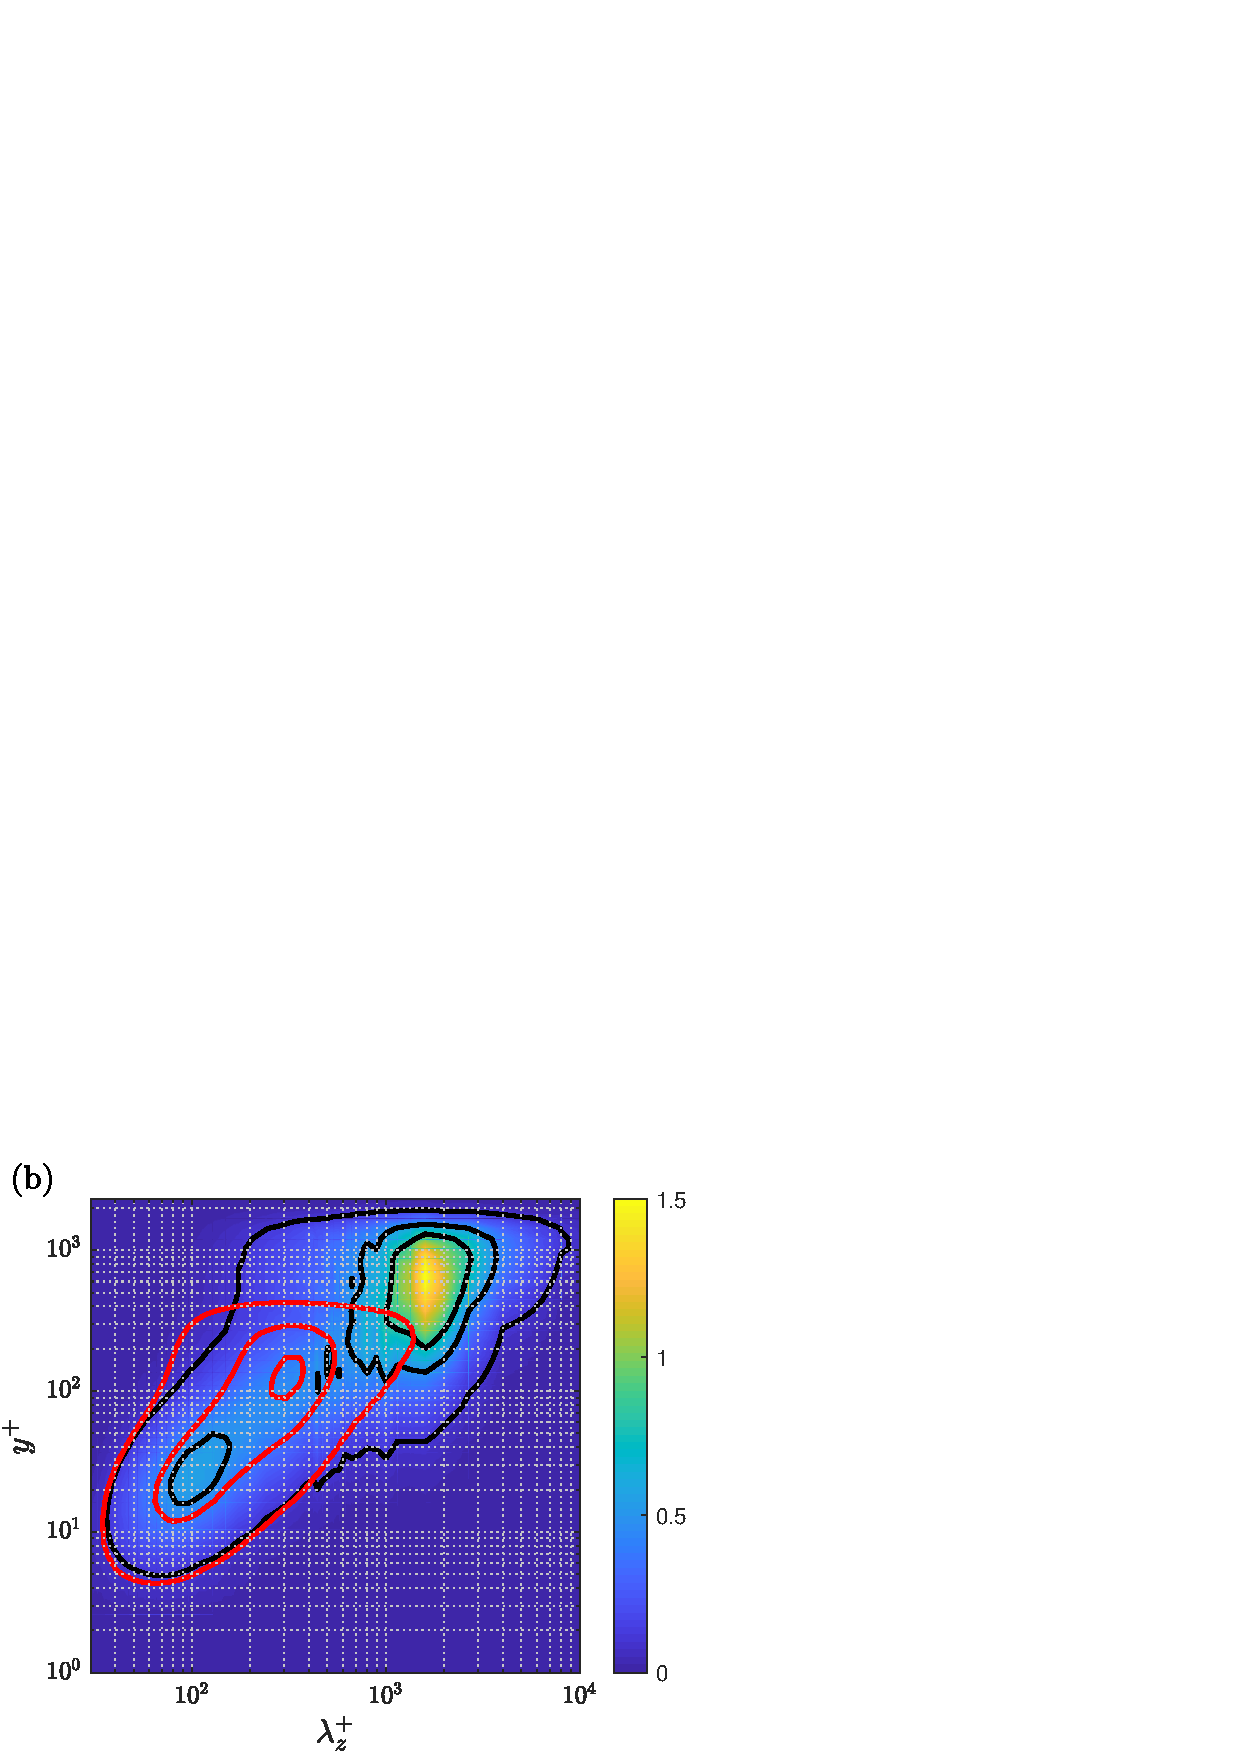
\includegraphics[width=0.48\textwidth]{APG_uv.jpg}
\caption{ \label{fig:ZPG_APG_Ret_500_2000_uv} Premultiplied spectrum $k_z\phi_{uu}$ and $|k_z\phi_{uv}|$ for (a)ZPG and (b)b1.4 simulations. Red contours at $\Rey_{\tau}=500$ and background and black contour are at a positions $\Rey_{\tau}=2000$. }
\end{figure}

The spectra shows a similar region of small-scale energy close to the wall which is responsible of the near-wall peak the RS $\overline{u\myprime u\myprime}$. The effects of $\Rey$ and $\beta$ increase the value of $\overline{u\myprime u\myprime}_{IP}^+$, even if the most of the spectra is similar for APG and ZPG at different Reynolds numbers.
The outer-spectral peak in $k_z\phi_{uu}$ is also responsible of most of the energy contained in the ZPG in the wake region, and increasing $\beta$ it increases the energy to the point of growing the outer peak in $\overline{u\myprime u\myprime}_{OP}^+$. This behaviour is similar in the other components of the RS tensor, where at higher $\Rey$ numbers there are larger and energetic scales acting on the wake region and influencing all across the TBL.

\subsection{Scaling of APG spectrum}

In \textbf{Paper 2} we try to understand the trends of the inner and outer peaks in $\overline{u\myprime u\myprime}$ shown in \textbf{Paper 1}. Why the inner scaled inner-peak grows with the Reynolds numbers and with the APG effects. Is it still correct to use viscous scaling?. 
We perform a scaling analysis of the different energetic scales of the power spectral density for both ZPG and APG simulations and at different Reynolds numbers.
First we start from the features observed in $k_z\phi_{u\myprime u\myprime}$ which are an spectral near-wall/inner peak (sIP) and an spectral outer peak (sOP). The data is scanned to look for the maxima at a certain wall-normal position and the maxima at a certain frequency. Since $k_z\phi_{u\myprime u\myprime}$ is saved in a rectangular matrix, it is equivalent to obtain the maxima along columns and the maxima along rows.
At high Reynolds number the separation of scales even in ZPG TBLs, allows to distinguish clearly the presence of 2 maximal points for $\Rey_{\tau}>500$. Other techniques could be used to detect the local maxima, but this method was obtaining satisfactory results, specially the values of $f(y)=max(k_z\phi(k_z, y))_{k_z}$ since that function presents less noise and it is shown in \highlight{ Fig.~\ref{fig:scaling_OP} figura de los escalados de los picos} that once the Reynolds number is enough to have separation of scales, the outer peak clearly separates in the wall-normal direction from the spectral near-wall peak.
Once sIP and sOP are located in $k_z\phi(k_z, y)$, (usually we represent with $\lambda_z$), we try the inner and outer length scalings used in \textbf{Paper 1} to scale $\overline{u\myprime u\myprime}(y)$.
It is shown that the viscous length $\ell_{\tau}$ scales the size of the spanwise scales of the sIP $\lambda_{z, sIP}^+$ as well as the wall-normal position $y^+_{sIP}$.
The same method is used for the spectral outer peak. The outer scales $\delta^*$ and $\delta_{99}$ were used to scale independently the wall-normal location $y_{sOP}$ and the size of the scales $\lambda_{z, sOP}$.
In previous studies such as \cite{Kitsios2017} the $\delta^*$ scaling was successful for the $y_{OP}$ as well as for $y_{sOP}$ at much higher $\beta$, however, $\lambda_z$ was also scaled with the same scaling.
In \cite{tanarro_2020}, the outer scaling was performed with $\delta_{99}$ for both $y$ and $\lambda_z$, and the values of $\lambda_{z,sOP}$ were better collapsed than using $\delta^*$ as in \cite{Kitsios2017}.
Taking into account this previous studies, we allowed $y$ and $\lambda_z$ to have different length scalings, and found the optimal collapse of the region around the spectral outer peak using $y/\delta^*$ and $\lambda_z/\delta_{99}$.

Once we obtained the scalings for the wall-normal position and size of the scales for both sIP and sOP, we looked the region around those peaks using the respective scalings, obtaining a good collapse, however there was another region to investigate, which is the region of small-scale energy in the wake region.
Different scalings were tried for $\lambda_z$ looking to match the vertical part of the energetic contours of the APG simulation at different $\Rey$.
We observed that using $\lambda_z/\delta^*$, there is a collapse around $\lambda_z/\delta^*=0.3$. It could be argued that the scaling evolves gradually at different $\lambda_z$ up to the region around the sOP that clearly scale using $\lambda_z/\delta_{99}$.
To have a better idea of how big was the contribution of the small-scale energy in the wake region, but also to understand what is the influence of the large scales in the near-wall region, we tried to accumulate the energy from small to large scales for all the wall-normal positions. In a matrix containing the $PS(y,k_z)$, this is equivalent to do a cumulative sum $cumsum(PS(y,k_z))_{k_z}$ along $k_z$.
In \cite{EAmorZPG}, they limited a rectangular region around sIP, to probe that inner scaled energy in this region does not vary with the Reynolds number, but we have seen that there are different scalings at different heights of the TBL, therefore, the rectangular domain to integrate over $\lambda_z$ and $y$ may not be the optimal tool for this analysis.

With the idea of looking for the contribution of small and large scales using a cumulative sum, and thinking that the accumulated energy would be in a certain scaling that probably would change with $\Rey$ effects, we thought of the percentual contribution of energy, or the marginal contribution of energy.
For a continuous PSD, the marginal contribution of energy (MCE) is defined as in Eq.~\ref{eq:MCE_cap2} and gives the percentual level of energy added by scales up to a wavenumber $k_{z,c}$ respect to the total value which would be $\overline{u_i\myprime u_j\myprime}$ at the same $y$.

\begin{equation}
\mathrm{MCE} = \int_{k_{z,c}}^{\infty} \phi_{u_iu_j} \mathrm{d} k_z \ \bigg/ \int_{0}^{\infty} \phi_{u_iu_j} \mathrm{d} k_z,
\label{eq:MCE_cap2}
\end{equation}

If we draw the $10\%, 20\%,...,$ contours, it is easy to show the regions where certain election of length and energy scales are valid, since the contours will be parallel where the scales contributes in the same way to the total RS. And they will start to diverge when the scaling is not appropriate.
Where the scaling is independent of $\Rey$, the contours for different $\Rey$ at the same MCE level in that region, will collapse, otherwise they will start to separate indicating for example that the influence of large-scale motions is affecting that region.
All of this is shown in \textbf{Paper 2} in more detail.
Answering why $\overline{u\myprime u\myprime}_{IP}^+$ grows with the $\Rey$ and $\beta$, the answer is that at higher $\Rey$ the influence of scales of size $\delta_{99}$ or larger, influence the near-wall region, and this influence is larger at with larger $\beta$. At this range of $\beta$, the viscous scaling is still valid, although certain modifications could be done taking into account the influence of the large scales.
At larger $\beta$, the flow is near-detachment and the viscous scaling is no longer applicable.




\begin{figure}[h!]
\centering
% \captionsetup{width=0.99 \textwidth}
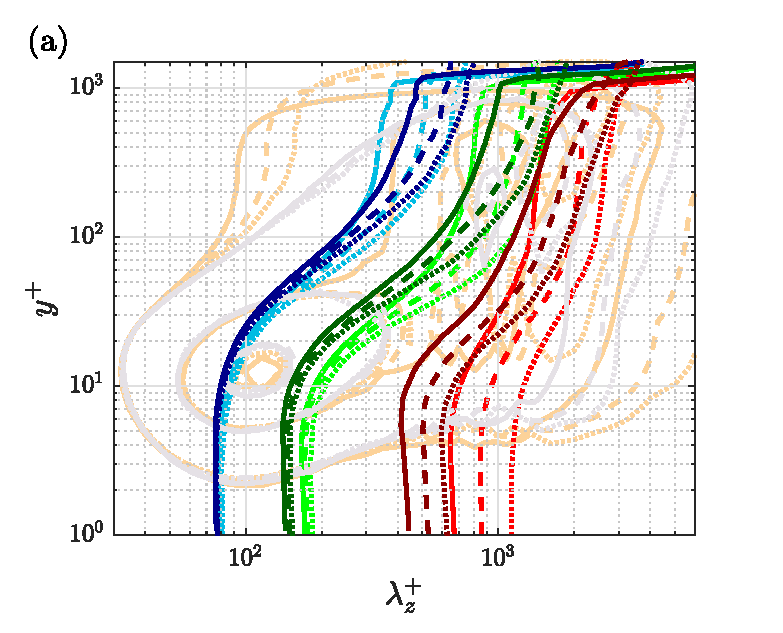
\includegraphics[width=0.45\textwidth]{imgs/spec/specMCE_uu_ltau_ltau.eps}
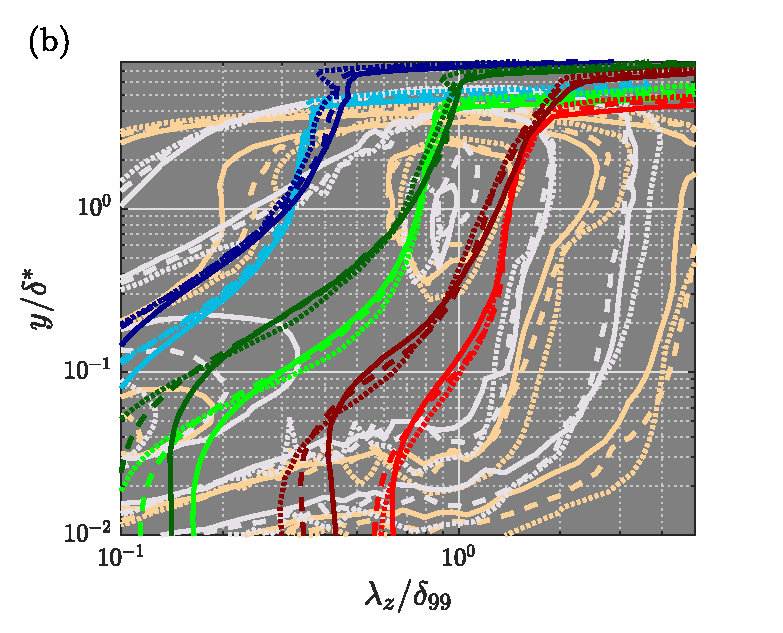
\includegraphics[width=0.45\textwidth]{imgs/spec/specMCE_uu_dstar_d99.eps}
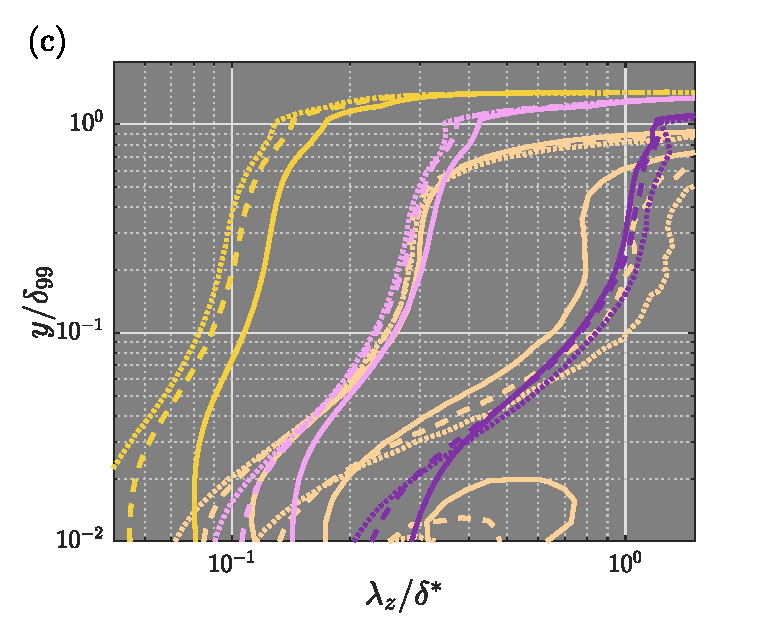
\includegraphics[width=0.45\textwidth]{imgs/spec/specMCE_uu_d99_dstar.eps}
\caption{ \label{fig:MCE_spec}
Contours of the premultiplied spectra $k_z\phi_{uu}$ in orange for b1.4 and light gray for the ZPG simulations.
The blue($20\%$), green($50\%$) and red($80\%$) lines are the MCE contours, where the light colors are used for the APG and the darker shades for the ZPG case.
Solid lines are used for $\Rey_{\tau}=1000$, dashed lines for $\Rey_{\tau}=1500$ and dotted lines $\Rey_{\tau}=2000$. Panel (a) shows the region that scales using inner scaling for both $y$ and $\lambda_z$; (b) scales the larger scales in the wake region by using two different length scales, $y\delta^*$ and $\lambda_z/\delta_{99}$. Panel (c) shows the scaling of the small-scale energy in the wake region characteristic of APGs, where $\lambda_z$ scales with $\delta^*$. The MCE contours are taken at $0.1\%$(yellow), $2.2\%$(pink) and  $15\%$(purple). 
}
\end{figure}







%===============================================================================
\chapter{Related Work}
%===============================================================================
%
%===============================================================================
\chapter{Conclusions and outlook}
%===============================================================================
%
%===============================================================================
\chapter{Test chapter, a very very very long title to test the table of contents}
%===============================================================================

This chapter is meant for testing the correct referencing of figures, equations
and tables.

% equations
%
\begin{equation}
	1 + 1 = 2
	\label{eq:test_eq1}
\end{equation}

\begin{align}
	2 + 2 = 4
	\label{eq:test_eq2}
\end{align}

\begin{equation}
	3 + 3 = 6
	\label{eq:test_eq3_intro}
\end{equation}

% tables
%
\begin{table}
	\centering
	\begin{tabular}{c}
		1
	\end{tabular}
	\caption{Test table 1}
	\label{tab:test_tab1}
\end{table}

\begin{table}
	\centering
	\begin{tabular}{c}
		2
	\end{tabular}
	\caption{Test table 2}
	\label{tab:test_tab2}
\end{table}

\begin{table}
	\centering
	\begin{tabular}{c}
		3
	\end{tabular}
	\caption{Test table 3}
	\label{tab:test_tab3_intro}
\end{table}

% figures
%
\begin{figure}[h!]
	\centering
	test figure 1
	\caption{Test figure 1}
	\label{fig:test_fig1}
\end{figure}

\begin{figure}[h!]
	\centering
	test figure 2
	\caption{Test figure 2}
	\label{fig:test_fig2}
\end{figure}

\begin{figure}[h!]
	\centering
	test figure 3
	\caption{Test figure 3}
	\label{fig:test_fig3_intro}
\end{figure}

% test references
%
\hrule
\begin{itemize}
	\item reference to equation 1: \eqref{eq:test_eq1}
	\item reference to equation 2: \eqref{eq:test_eq2}
	\item reference to equation 3: \eqref{eq:test_eq3_intro}
\end{itemize}
\hrule
\begin{itemize}
	\item reference to table 1: \eqref{tab:test_tab1}
	\item reference to table 2: \eqref{tab:test_tab2}
	\item reference to table 3: \eqref{tab:test_tab3_intro}
\end{itemize}
\hrule
\begin{itemize}
	\item reference to figure 1: \eqref{fig:test_fig1}
	\item reference to figure 2: \eqref{fig:test_fig2}
	\item reference to figure 3: \eqref{fig:test_fig3_intro}
\end{itemize}
\hrule

%===============================================================================
% Acknowledgments
%===============================================================================
%
\begin{acknowledgements}
% 	We would like to thank Gigi and SCIgen - An Automatic CS Paper Generator%
% 	\footnote{\url{https://pdos.csail.mit.edu/archive/scigen}}.
I would like to thank Ricardo Vinuesa and Philipp Schlatter first, without them I wouldn't have lived this wonderful adventure
which was to conduct my PhD studies in KTH. 
Qiang Li, a collaborator in my publications, but also a mentor, always encouraging me and ready to help. They have helped and guided me through my academic work and have always been there to share their knowledge an experience.
I also have to thank all those PhD's and professors that have made the life in the office so wonderful, in spite of the huge change that covid brought to our lifes.
Luca, Simon, Valerio and Vitor, with whom I lived my first "western" adventure. And the list goes on and on.
My family and friends in Spain that missed me so much, and my small "family" in Sweden for your moral support in good and dark times.
\end{acknowledgements}



%===============================================================================
% References
%===============================================================================
%
\bibliographystyle{jfm}
\bibliography{thesis}
%
% \IfFileExists{overview.bbl}{\graphicspath{{imgs/}}

%===============================================================================
\chapter{Introduction}
%===============================================================================
%
Throughout my academic career, I have enjoyed the step-by-step process of learning and I have discovered a passion for sharing my knowledge with friends, colleagues and some of my students.
In the same way the process of learning is unique, the process of teaching or communicating the knowledge should also be personal, trying to achieve the main goal of communication, transmitting correct information.
When we try to learn about a subject we can go to books, classes, different teachers, publications..., and sometimes we understand better from a book, other times from a video or a specific teacher or friend.
In this thesis, I will present some results on the physics of turbulent fluid mechanics where I have been involved, and I will try my best to communicate this knowledge to those interested in reading this work even if the reader is not very familiar with fluid dynamics.
Ideally, this transmission of knowledge should be concise, but I have experienced that certain complex knowledge sometimes requires different points of view or a simpler language. Personally, I like to communicate my knowledge as if it was a conversation instead of formal and impersonal writing.

Fluid mechanics or dynamics may sound as something complex for the non initiated, and it really is a complex science, but we already have intuitive and practical knowledge since we live and manipulate fluids every day so I will explain the basics.

A fluid is a substance that in contrast with a solid, it can easily deform and this property allows for the substance to adapt to containers or to move around other obstacles. An example is the air of the atmosphere, the liquid water in the sea, and even solids, like large accumulations of fine sand which subjected to vibrations can behave similar to liquid water.
Fluid mechanics is the science that studies everything related to the movement of fluids, like the forces involved or the properties of the fluid in its motion.

When a fluid moves around a solid (water around a rock), or the solid moves immersed in a fluid  (car moving through the air of the atmosphere) the fluid adapts to that relative motion by changing its properties, such as the velocity of its particles.
Where the fluid meets the solid, its particles have the same velocity as the solid because the forces in the interface fluid-solid (friction and pressure forces) are enough to deform the fluid.
The viscosity is the property of the fluid that opposes to the deformation. Inside the fluid, the viscosity is seeing as a force that reduces the velocity of the deformation or the velocity of the fluid particles.
In the example of the water in a river moving around a rock, far from the rock, the velocity of the water is that of the river, however the water in contact to the rock is not moving according to what we have explained earlier. The viscosity is responsible to adapt the velocity of the fluid from the velocity of the river to the velocity of the rock.
The change of velocity is actually done in a very small distance, and this region where the viscosity forces are adapting the fluid velocity is called boundary layer. 
The idea of boundary layer was introduced by Ludwig Prandtl in 1904 and it is the main topic of this thesis.

The boundary layers studied here are those pertaining to the momentum of the flow. The interest is in the effects of adverse pressure gradients in well-developed turbulent boundary layers. To avoid the influence of other effects we consider the simplest scenario.
The fluid is isotropic, incompressible and Newtonian, therefore the temperature does not change the density and the viscosity of the fluid.

The simplest solid boundary used is a flat plate without any heat or mass exchange (no suction or blowing). The adverse pressure gradient is then imposed as an outer boundary condition.
Comparisons can then be done with curved-boundary solids such as NACA profiles, where the pressure gradients are an aftereffect of the curvature of the profile. 
In these realistic configurations different mechanisms to control the flow are applied such as blowing or suction.

For these simple configurations we use a Cartesian system of coordinates where the space is denoted with $\vec{x}=x_i=(x,y,z)$, where we show the vectorial, dyadic and coordinate notations that will be used.
The boundary layers studied here are statistically 2D, $y$ is the wall-normal direction, $z$ is the homogeneous direction and $x$ is chosen as the streamwise direction. The time is denoted with $t$.
Although turbulence is a 3-dimensional (3D) phenomena, the flow analysed is statistically 2-dimensional, since there is an homogeneous direction. 

%-------------------------------------------------------------------------------
\section{Our Contribution}
%


\thesisstructure Add here a brief description of the structure of the thesis.

%===============================================================================
\chapter{Boundary layers, turbulence and pressure gradients}
%===============================================================================
%
% \begin{enumerate}
%     \item Physical phenomena
%     \begin{enumerate}
%         \item Elements involved (fluid and solid)
%         \item Properties of the elements that are meaningful for the problem
%         \item Observations or experimental knowledge $\rightarrow$ effects observed
%         \item New unseen problem $\rightarrow$ hypothesis of the effects to be observed
%     \end{enumerate}
    
%     \item Abstraction of the problem at hand and the physics
%     \begin{enumerate}
%         \item Equations for the physics studied (mechanics, thermal?, chemical?)
%         \item Mathematical model of the elements properties
%         \item Outer factors or conditions
%     \end{enumerate}
%     \item Analytical solution or numerical discretization.
%     \item Validation with experimental results
% \end{enumerate}

\graphicspath{{imgs/} {imgs/lam_turb} {imgs/spec}}

\section{Observations and empirical knowledge}

There are many examples of laminar and turbulent flows in nature that we are familiar with. In Fig.~\ref{fig:lam_turb} we show 3 examples, with water and flames. In the river image the water on the right side is laminar and on the left side it becomes turbulent. The calm flames of a candle rise initially in a laminar regime. On the bonfire example the flames are larger and show the different chaotic scale motions of a turbulent flow.

\begin{figure}[h!]
\centering
% \captionsetup{width=0.99 \textwidth}
\includegraphics[height=5cm ]{laminar_turbulent_1.jpg}
% \includegraphics[width=5cm ]{llama_laminar.jpg}
\includegraphics[height=5cm ]{velas.jpg}
\includegraphics[height=5cm ]{llama_turb1.jpg}
\caption{ \label{fig:lam_turb} Examples of ordered laminar flow and chaotic turbulent motions in water and fire.
   }
\end{figure}

Laminar and turbulent regimes presents its advantages and disadvantages. 
In aerodynamic applications we usually focus in minimizing the friction produced at the solid wall-boundary or maximizing the lift/drag coefficient. In that aspect, the laminar boundary layer produces less friction than a turbulent boundary layer because it alters less the flow.
Detachment of the flow is an undesirable effect produced by strong adverse-pressure gradients, in this aspect, the laminar flow structure is more sensible to detachment under APG conditions than a turbulent flow.

To study turbulent boundary layers (TBLs) and the effects of adverse pressure gradients (APG) we will compare APG TBLs with a TBL subjected to zero pressure gradient (ZPG) conditions. The case of favourable pressure gradients (FPGs) stabilizes and relaminarizes the boundary layer, and its effects are not critical such as those provoked by APGs, where the boundary layer can detach from the wall producing undesirable effects such as an increase in drag or even to loose the aerodynamic controls in airplanes.
In order to study this kind of wall-attached fluid problem, first we should analyze the elements involved, such as the fluid and the solid elements.

\section{Fluid properties}

When studying the mechanics of a solid we track the positions, velocities and accelerations, forces and torques along its movement in space and time. This is the Lagrangian approach to mechanics.
For a flow of particles or a fluid it is more interesting to observe the flow variables at specific locations and observe the temporal change of those variables at those locations. This is the Eulerian approach that will be used to study the mechanics of a fluid flow. 

The main variables are the fluid velocities, $\vec{u}(\vec{x},t)=u_i=(u,v,w)$, and the pressure $p(\vec{x},t)$.
To simplify the study of adverse pressure gradient turbulent boundary layers the fluid analysed is isotropic (its properties are the same in all directions) and Newtonian, this implies that the viscous forces are a linear function of the strain rate tensor $s_{ij}=\pdv{u_i}/{x_j}$. As an example, the friction at the wall is $\tau_w=\mu \pdv{u}/{y}$
where $\mu$ is a constant factor, the dynamic viscosity.
The density and viscosity of the fluid combines into the kinematic viscosity $\nu=\mu/\rho$ with units $[m^2/s]$ independent of the mass. 
Since we consider the density and viscosity as constant and not affected by changes in temperature, the temperature of the fluid is not relevant and the energy and momentum evolution are decoupled.

\section{Solid properties}
In general, the solid boundaries are curved specially in aerodynamic applications where the curvatures are used to create differences in pressures that lead to forces in the desired directions. The forces in the direction of the inflow are called drag and the forces in the perpendicular direction is called lift. For curved boundaries, different coordinate systems are used. The local system of coordinates that changes with the solid boundary is where the surface forces are calculated. The surface forces are then projected onto the global coordinates associated with the inflow to obtain the lift and drag.
For flat plates with zero angle of attack the global and local coordinates are the same.
The surface of the flat plate that we study is rigid, and smooth, and no exchange of heat or mass is produced between the fluid and the solid. In the interface fluid/solid the only interaction is due to pressure and viscous forces that adapts the fluid velocity to the solid surface velocity.
The flat plate will be considered to be static in the global system of coordinates.


\section{Boundary layers}

Boundary layers are regions inside a fluid flow where certain features or changes in the properties of the fluid are concentrated. Historically the first idea of boundary layer is set for the adaptation region of the fluid momentum from outer conditions to the dynamical conditions in a solid surface.
Other boundary layers are for example thermal boundary layers where the focus is on the change of thermal properties.

When we consider the flow around a solid object in an incompressible regime, the flow can detect the presence of the solid object and adapt its trajectory. The flow then surrounds the solid starting from the leading edge and close to the solid surface the boundary layer is the region where the velocity of the flow adapts from the solid surface velocity to the outer flow velocity. The boundary layer thickness have to be defined according to the main idea of a region of the fluid close to the solid wall that encloses the major viscous effects created due to the fluid/surface interaction. An obvious effect of the presence of a wall is that the streamwise velocity has to adapt from the velocity of the solid boundary to the exterior velocity, commonly called velocity at the infinity $U_{\infty}$. 
In general, for a certain position of the wall, the velocity is measured in the wall-normal direction, obtaining a profile of streamwise velocities $u(y,t)$. Then $U_{\infty}=u(y\rightarrow \infty)$ is the unperturbed velocity and can change from one streamwise position to another.
In the case of zero-pressure gradient boundary layers, $U_{\infty}$ is taken as constant, since in a steady flow in the absence of viscous forces, $\pdv{u}/{x}$ should be zero. 

Since an obvious indicator of the boundary layer is the adaptation of the streamwise velocity, the boundary layer can be defined using this property and the $99\%$ thickness $\delta_{99}$ is defined as the wall-normal position where $u(y=\delta_{99}) = U_{\infty}$.
In Fig.~\ref{fig:lam_turb_profiles} we show an example on how the mean streamwise velocity $U(y)$ adapts from the velocity at the wall $u(y=0)=0$, to the outer velocity $U_{\infty}$, which has been scaled to be equal to 1, on a laminar and a TBL ZPG profiles.

\begin{figure}[h!]
\centering
% \captionsetup{width=0.99 \textwidth}
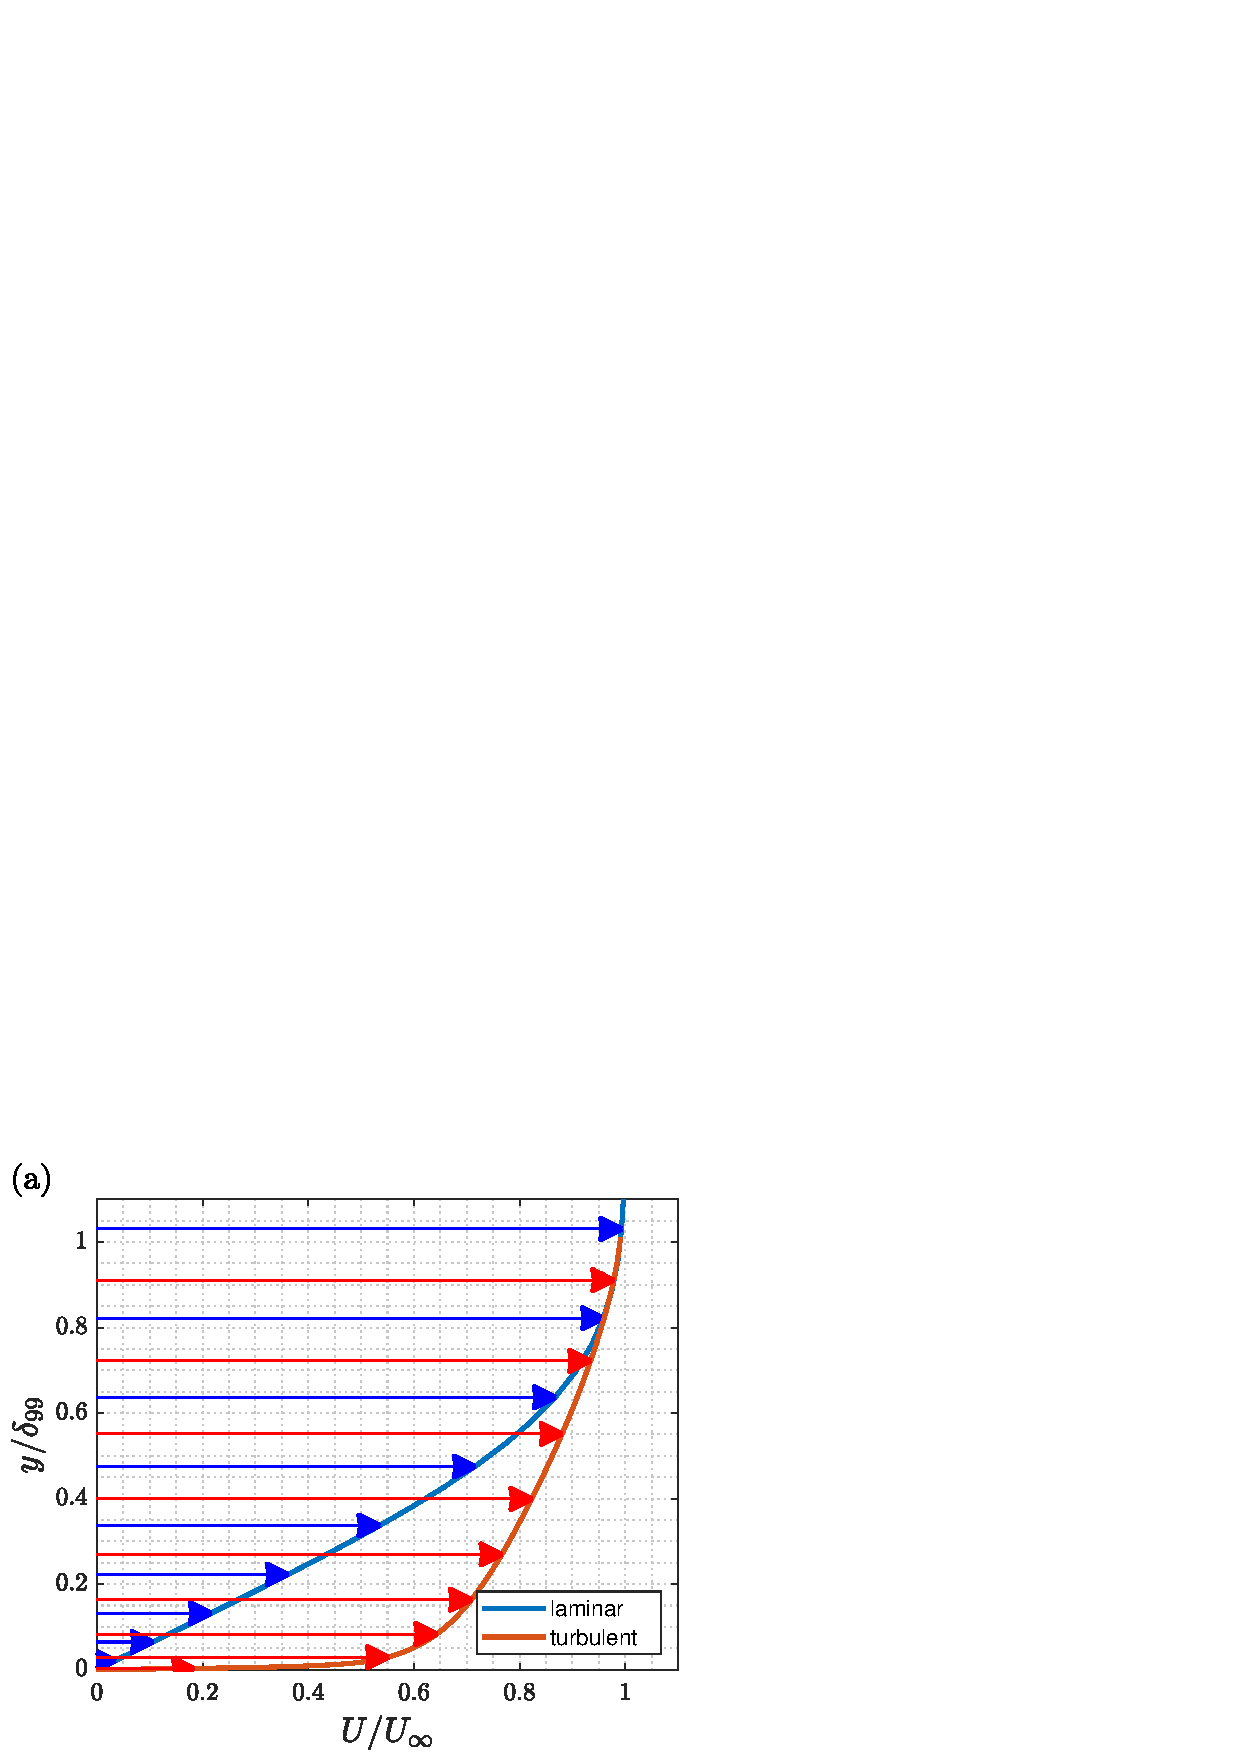
\includegraphics[width=0.5\textwidth]{ZPG_lam_turb.jpg}
\caption{ \label{fig:lam_turb_profiles} Mean streamwise velocity profile of a laminar (blue) and a turbulent ZPG (red) boundary layers.
   }
\end{figure}

In the case of curved boundaries, the curvature induces a pressure-gradient since the incoming flow has to adapt to the curvature of the wall. In a flat plate, a pressure-gradient can be produced by controlling the exterior flow, usually the streamwise gradient of the streamwise velocity $\pdv{U_{\infty}}/{x}$


\subsection{Turbulent boundary layers}
The characteristics of a boundary layer changes radically depending on the laminar/turbulent regime.
In a laminar boundary layer, any perturbation produces shear stresses and therefore, viscous forces, which are transported by the momentum of the flow and eventually dissipated by the viscous dissipation. 
High energetic perturbations, flow configurations or certain viscosity/momentum forces ratios are unstable, implying a change of regime, usually from the laminar regime to turbulence. 
The ratio between momentum and viscous forces is called Reynolds number $\Rey=U_{sc} L_{sc} / \nu$ and depending on the velocity scale $U_{sc}$ and the $L_{sc}$ chosen we would be analyzing different phenomena. The Reynolds number where a fluid configuration changes regime is called critical Reynolds number $\Rey_c$.
Other Reynolds number examples: if $U_{sc}=U_{\infty}$ and $L_{sc}=c$ where $c$ is the chord of a NACA profile, then we are setting the global configuration of the problem. If we want to analyze a local phenomena such as the different size of the fluid scales close to the wall compared to the largest ones inside the TBL, then we can use the Reynolds number based on the friction velocity $\Rey_{\tau}=u_{\tau}\delta_{99}/\nu$, where  $u_{\tau}(x)=\sqrt{(\tau_w / \rho)}$.

In the turbulent regime, the momentum and energy of the flow initiates a cascading effect breaking the initial ordered motions into chaotic submotions. 
Eddies are generated that extract energy from the mean flow and are divided into smaller eddies. Then a transport of energy between large and small eddies is produced. Eddies are regions with strong shear stresses, therefore the viscous forces are stronger and produce a dissipation of the kinetic energy.
The boundary layers studied here are momentum boundary layers that confine the turbulent perturbations and mayor viscous effects produced because of the presence of a solid boundary.

In a turbulent boundary layer, the thickness of the boundary layer should capture both the effects of the viscous forces as well as the turbulent fluctuations produced because of the presence of a solid boundary, leading to different definitions for the boundary layer thickness.

For laminar BLs and ZPG TBLs, the previous $\delta_{99}$ thickness, where the mean velocity of the flow is $99\%$ of the exterior velocity, is valid and is based only on the adaptation of the mean streamwise velocity to that of the outer flow.

For other TBLs with pressure gradients, the outer velocity can have gradients in the streamwise and wall-normal directions even without the presence of turbulence. In this case we can use an approach based on the level of turbulence such as the one used in \cite{diagnostic_Vinuesa} where the boundary layer thickness is such that it captures the turbulence up to certain turbulent level.
This approach is useful for the dataset that we use, since the turbulent levels outside of the TBL are minimal, both in the simulations \citep{E-AmorZPG, bobke2017, Pozuelo_JFM_22}, as in the experimental databases \citep{Sanmiguel_PRF}.
If the outer flow turbulent level is high, the method in \cite{diagnostic_Vinuesa} is not applicable. 
Other methods have been proposed in the literature and a review was given in \cite{d99_determination_2020}.

Turbulence presents a wide range of motions, the way we have been able to study and characterize turbulence is through decomposition of those characteristics. 
The first approach is an statistical characterization where we can divide the fluid variables into a mean or average value and a perturbation, this is known as the Reynolds decomposition \citep{Rey_decomp}.
The fluctuating character of the flow is shown for a flat plate APG TBL in Fig.~\ref{fig:lam_turb_development} where we show contour levels in snapshots of the instantaneous streamwise velocity. The contours in Fig.~\ref{fig:lam_turb_development}(a) are smooth and show a well-defined laminar behaviour with small perturbations introduced to trigger turbulence. In Fig.~\ref{fig:lam_turb_development}(b) the turbulence is totally developed It can be seen how at different streamwise positions $x/\delta^*_0$ the outer velocity or "edge velocity" $U_e$ decreases along $x$ to obtain an APG. The edge velocity is the velocity of the TBL at $y=\delta_{99}$ and depends on the method used to determine the boundary layer thickness.

\begin{figure}[h!]
\centering
% \captionsetup{width=0.99 \textwidth}
\includegraphics[width=0.49\textwidth ]{APG_laminar.jpg}
\includegraphics[width=0.49\textwidth]{APG_turb.jpg}
\caption{ \label{fig:lam_turb_development} Snapshot of the streamwise velocity $u(\vec(x), t)$ in a laminar (a) and a turbulent APG (b), boundary layers.
   }
\end{figure}



\section{Mathemathical analysis}

For an incompressible flow the conservation of mass in a control volume becomes the differential continuity equation (Eq.~\ref{eq:continuity_cap2}),

% Continuity
\begin{equation}
\label{eq:continuity_cap2}
% \overrightarrow{u}
    \nabla \cdot \vec{u} = \partial_i u_i = 
    \frac{\partial u}{\partial x} + \frac{\partial v}{\partial y} + \frac{\partial w}{\partial z} = 0,
\end{equation}
which is shown as the divergence of the velocity vector, the diadic and components notations.

To describe the time evolution of the fluid variables, the partial differential equations in Eq.~\ref{eq:NS_cap2} are the Navier--Stokes (NS) equations that describes the evolution of the momentum of the fluid as a function of the pressure gradient and viscous forces acting on it. The system of equations composed by Eqs.~\ref{eq:continuity_cap2} and \ref{eq:NS_cap2} are able to give both laminar and turbulent flow regimes, depending on the configuration of the problem.

% NS Total velocities
\begin{equation}
    \label{eq:NS_cap2}
    \frac {\partial u_i} {\partial t}  + u_j \frac {\partial u_i} {\partial x_j} =
    \frac {-1} {\rho} \frac {\partial p} {\partial x_i} +  \nu \frac {\partial^2 u_i} {\partial x_j^2}.
\end{equation}

By giving the correct scenario which is the boundary conditions (BCs) composed by an inflow, outflow, outer flow and wall-boundary conditions, together with an initial state of the system, we can expect either laminar flow or the change into a turbulent flow.



Once turbulence is fully-developed, the statistical approach to turbulence is based on the Reynolds decomposition \citep{Rey_decomp}, given in Eq.~\ref{eq:Rey_decomp}. This decomposition is based on a constant or averaged component and a fluctuating component in a way that once they are inputted into Eqs.~\ref{eq:continuity_cap2} and \ref{eq:NS_cap2} some of the partial differentials are simplified. An example is to use a constant base flow (such as the laminar state) plus a fluctuating flow field, this is the case used to study transition and stability of BLs. 
For our case, the mean flow $U_i$ is an average in time and the homogeneous directions. The average in a dimension $d$ is marked as $\langle . \rangle_d$, and the average in time and all the homogeneous dimensions is marked with $\overline{(.)}$. The mean velocity is $U_i = \overline{u_i} =\langle \langle u_i \rangle_z \rangle_t$ and as a result of Eq.~\ref{eq:Rey_decomp}, $\overline{u_i\myprime}=0$. Note that $\langle u_i\myprime \rangle_z (t) \neq 0$ and $\langle u_i\myprime \rangle_t(z) \neq 0$. 

Introducing the flow decomposition (Eq.~\ref{eq:Rey_decomp}) into the continuity and NS equations (Eqs.~\ref{eq:continuity_cap2} $\&$ \ref{eq:NS_cap2}), and using the total average in time and $z$, we see that the continuity equation is fulfilled for both the mean and the fluctuating component separately (Eq.~.\ref{eq:cont_decomp}). And in the NS equation we obtain the Reynolds Averaged Navier--Stokes equation (RANS) in Eq.~\ref{eq:RANS_cap2} and the equation for the time evolution of the perturbations Eq.~\ref{eq:pertub_cap2} as a result of substracting the RANS equations from the general NS equations.

% R Decomposition
\begin{equation}
    \label{eq:Rey_decomp}
    u_i = U_i + u_i\myprime.
\end{equation}

\begin{equation}
    \label{eq:cont_decomp}
    \partial_i \overline{u_i} = \partial_i \overline{U_i} = 0 ~~~~
    \partial_i \overline{U_i} + \partial_i \overline{u_i\myprime} = 0.  
\end{equation}

% RANS
\begin{equation}
    \label{eq:RANS_cap2}
    U_k\pdv{U_i}{x_k} + \pdv{\overline{u_i\myprime u_k\myprime}}{x_k} = \frac {-1} {\rho} \frac {\partial P}{\partial x_i} + \nu  \frac {\partial^2 U_k} {\partial x_k^2}.
\end{equation}

% Perturbations
\begin{equation}
    \label{eq:pertub_cap2}
    {\pdv{u_i\myprime}{t} + 
    U_k\pdv{u_i\myprime}{x_k} + u_k\myprime\pdv{u_i}{x_k} - \pdv{\overline{u_i\myprime u_k\myprime}}{x_k}  =
    \frac {-1} {\rho} \pdv{p\myprime}{x_i} + \nu  \frac {\partial^2 u_k\myprime} {\partial x_k^2}    }.
\end{equation}

Note that the RANS equation are similar to the NS equation, except that for the time derivative which is zero and an aditional term $\pdv{\overline{u_i\myprime u_k\myprime}}/{x_k}$ which can be included within the divergence of the viscous forces term, for that reason the terms $\rho \overline{u_i\myprime u_k\myprime}$ are called Reynolds-stresses. In the following, since the density is considered as constant, we will refer as Reynolds-stress (RS) to the terms in the tensor $\overline{u_i\myprime u_k\myprime}$, wich are also known as the variance or covariance of the total velocities $u_i$, $u_k$.
From the RANS equations it is interesting to see the mean velocities and the RS terms since they are an indicative of the level of turbulence and how it is affected by the pressure gradients and viscous forces on the right hand side (RHS) of the equation.

The equation for the perturbation velocities is useful since we can multiply by another perturbation velocity such as $u_{j}\myprime \cdot \left( \pdv{u_{i}\myprime}{t} + ... \right) $ or obtain the two-point correlation $\mathcal{R}_{u_i\myprime u_j\myprime}$ through the correlation denoted with the symbol $(\cdot \star \cdot)$ as in $ u_{i}\myprime \star \left( \pdv{u_{j}\myprime}{t} + ... \right)$. The former gives the Reynolds-stress transport equations (Eq.~\ref{eq:RS_transport_cap2}) where the turbulent kinetic energy budgets are a special case. The latter is used as in \cite{lee_moser_2019}, to obtain the power spectral density of each term of the Reynolds-stress transport equations.

Denoting Eq.~\ref{eq:NS_cap2} as $\mathrm{TOT}_i$, Eq.~\ref{eq:RANS_cap2} as $\mathrm{RANS}_i$ and Eq.~\ref{eq:RS_transport_cap2} as $\mathrm{PERT}_i$, the evolution equation for the total kinetic energy of the flow can be obtained through the multiplication,
% $\mathrm{KE} = (1/2) \overline{u_i \cdot \mathrm{TOT}_i}$, 
\begin{equation}
    \mathrm{KE} = (1/2) \overline{u_i \cdot \mathrm{TOT}_i}, 
\end{equation}
while the mean kinetic energy equation can be obtained with 
% $\mathrm{MKE} = (1/2) U_i \cdot \mathrm{RANS}_i$,
\begin{equation}
    \mathrm{MKE} = (1/2) U_i \cdot \mathrm{RANS}_i,
\end{equation}
and the turbulent kinetic energy equation with 
% $\mathrm{TKE} = (1/2) \overline{u_i\myprime \cdot \mathrm{PERT}_i} = KE - MKE$.
\begin{equation}
    \mathrm{TKE} = (1/2) \overline{u_i\myprime \cdot \mathrm{PERT}_i} = KE - MKE.
\end{equation}
In a similar way the Reynolds-stress transport ($RST_{ij}$) equation Eq.~\ref{eq:RS_transport_cap2} can be obtained by doing 
% $\mathrm{RS}_{ij} = \overline{u_i\myprime \cdot \mathrm{PERT_j} + u_j\myprime \cdot \mathrm{PERT_i}} $
\begin{multline}
    \mathrm{RST}_{ij} = \overline{u_i\myprime \cdot \mathrm{PERT_j} + u_j\myprime \cdot \mathrm{PERT_i}} = \\
    = \overline{u_i \cdot \mathrm{TOT_j} + u_j \cdot \mathrm{TOT_i}} - (U_i \cdot \mathrm{RANS}_j + U_j \cdot \mathrm{RANS}_i ) .
\end{multline}
% $\mathrm{RS}_{ij} = \overline{u_i \cdot \mathrm{TOT_j} + u_j \cdot \mathrm{TOT_i}} - (U_i \cdot \mathrm{RANS}_j + U_j \cdot \mathrm{RANS}_i )$.
% \begin{equation}
%     \mathrm{RS}_{ij} = \overline{u_i \cdot \mathrm{TOT_j} + u_j \cdot \mathrm{TOT_i}} - (U_i \cdot \mathrm{RANS}_j + U_j \cdot \mathrm{RANS}_i ) .
% \end{equation}

% RS transport equation
\begin{multline}
    \label{eq:RS_transport_cap2}
    \pdv{\overline{u_i\myprime u_j\myprime}}{t} + 
    U_k\pdv{\overline{u_i\myprime u_j\myprime}}{x_k} + 
    \left(
    \overline{u_i\myprime u_k\myprime}\pdv{U_j}{x_k} + \overline{u_j\myprime u_k\myprime}\pdv{U_i}{x_k}
    \right) +
    \left(
    \overline{u_i\myprime \pdv{u_j\myprime}{x_k} u_k\myprime} + \overline{\pdv{u_i\myprime}{x_k} u_j\myprime u_k\myprime}
    \right)
    = \\ 
    - \left( \overline{
    u_j\myprime \pdv{p\myprime}{x_i} + u_i\myprime \pdv{p\myprime}{x_j}
    } \right) 
    + \nu \frac{\partial^2 \overline{u_i\myprime u_j\myprime}}{\partial x_k^2} 
    - 2\nu \overline{\pdv{u_i\myprime}{x_k} \pdv{u_j\myprime}{x_k}}
\end{multline}

The third term in Eq.~\ref{eq:RS_transport_cap2} is specially interesting, after some manipulation, that term appears in the transport of $U_iU_j$ and the transport of $\overline{u_i\myprime u_j\myprime}$ with different signs. Usually is written on the right hand side of the equation and is called ``Production" since it substract energy from the mean flow and adds into the perturbations.
The other terms are presented in Appendix B from \textbf{Paper 1}.



%===============================================================================
\chapter{Numerical experiments on flat plate turbulent boundary layers}
%===============================================================================
%

\section{Turbulent Boundary layers under adverse pressure gradients}

A wall-bounded flow can see pressure gradients as a result of the curvature of the wall, but also as a result of a change in the direction/velocity of the outer flow $(U_{e}, V_{e}, W_{e})$. Turbulence is already a complex problem in a ZPG case with the only parameter being the Reynolds number (momentum/viscous forces), if another parameter such as pressure gradients is added, the complexity of the problem increases and it becomes difficult to distinguish what phenomena is caused by the $\Rey$ effects or by the PG history of the flow.
In order to properly study APG TBLs, first we should try to define a canonical simple case, that is a well-defined APG along the streamwise development of the TBL, this is what we refere as the PG history of the flow.
To address this problem, different pressure-gradient parameters have been defined in literature, such as the Rotta-Clauser PG parameter $\beta$, or a general $\Lambda_{inc}$ which in \cite{Gibis2019} is studied with different length and velocity scales.
In our simulations of moderate APGs we have used $\beta$ defined as
\begin{equation}
    \beta(x) = \frac{\delta^*}{\tau_w} \pdv{P}{x},
\end{equation}
where $\pdv{P}/{x}$ is the averaged pressure-gradient, $\tau_w$ is the mean shear stress at the wall, and $\delta^*$ is the displacement thickness, which for an incompressible flow is defined as
\begin{equation}
    U_e \delta^* = \int_{0}^{\delta_{99}} (U_e - U) dy
\end{equation}

% IDEA behind beta
The idea behind the $\beta$ parameter is to stablish an integral equilibrium of forces across the TBL, in this way, every section of the TBL is subjected to the same dimensionless state of forces.
To clear this idea, Fig.~\ref{fig:scheme_beta} shows a scheme of a section of the BL, where the main forces are due to the streamwise pressure-gradient and the stress at the wall.

\begin{figure}
    \centering
    \includegraphics[width=0.90\textwidth]{imgs/schemes/scheme_beta.jpg}
    \caption{Stresses around a section of a BL.}
    \label{fig:scheme_beta}
\end{figure}

Integrating the streamwise momentum equation over the wall-normal direction, under several assumptions, it is possible to obtain an equation which relates the integral parameters $\delta^*$, $\theta$ and $\beta$, therefore, from an integral approach, the thickness $\delta \myprime$ is chosen equal to $\delta^*$. 



\section{Statistics}
In \textbf{Paper 1} we explore the statistical quantities of TBLs under APGs. The novelty respect to the available literature was in the high fidelity database used for the ZPG and APG TBLs. Both simulations show the development of the TBL from low Reynolds numbers such as those of previous numerical databases, and reach large Reynolds numbers such as those obtained in experiments. This characteristic works as a bridge to validate previous simulations as well as the current simulations, since they have been compared successfully with experimental data.
A benefit of numerical experiments is that the amount of quantities measured are larger than in experimental databases. This allows to have better measurements close to the wall and obtain decomposition such as spanwise spectra.

\begin{table}
  \begin{center}
  \fontsize{8.0pt}{10.25pt}\selectfont
  \addtolength{\tabcolsep}{-2pt}
\def~{\hphantom{0}}
    \begin{tabular}{ l r  r  r }
    Case  & Colour & Reference \\[3pt]
    \hline
    b1             & \redline     & Bobke (\citeyear{bobke2017}) \\
    b2             & \greenline   & Bobke (\citeyear{bobke2017}) \\
    m16            & \blueline    & Bobke (\citeyear{Bobke_2016}) \\

    ZPG            & \blackline   & Eitel-Amor (\citeyear{E-AmorZPG}) \\
    b1.4           & \orangeline  & Pozuelo (\citeyear{Pozuelo_JFM_22}) \\
    exp            & \redcircle   & SanMiguel (\citeyear{MTL_expSANMIGUEL}) \\
    \hline
    \end{tabular}
  \caption{ Line styles and colors used for the simulations and experiments used in the thesis.}
  \label{tab:param_cap2}
  \end{center}
\end{table}

% \begin{table}
%   \begin{center}
%   \fontsize{8.0pt}{10.25pt}\selectfont
%   \addtolength{\tabcolsep}{-2pt}
% \def~{\hphantom{0}}
%     \begin{tabular}{ l r  r  r  r  r  r  r  r  r  r  r r}
%     Case  & $L_x/\delta_0^*$ & $L_y/\delta_0^*$ & $L_z/\delta_0^*$ & $m_{x}$ & $m_{y}$ & $m_{z}$ & $\Delta x^{+}$ & $\Delta y_{\rm max}^{+}$ & $\Delta z^{+}$ & Colour & Reference \\[3pt]
    
%     b1             &    3000   &   140   &    250  &    3072 &     301 &     576 &   21.8    & 8.4 &   9.7  & \redline     & Bobke (\citeyear{bobke2017}) \\
%     b2             &    3000   &   180   &    320  &    3072 &     361 &     768 &   21.6    & 7.9 &   9.2  & \greenline   & Bobke (\citeyear{bobke2017}) \\
%     m16            &    3000   &   180   &    220  &    3072 &     361 &     576 &   21.2    & 7.7 &   8.3  & \blueline    & Bobke (\citeyear{Bobke_2016}) \\

%     ZPG            &   13500   &   400   &    540  &   13824 &     513 &    1152 &   22.6    & 19.6 &  10.9  & \blackline  & Eitel-Amor (\citeyear{E-AmorZPG}) \\
%     b1.4           &   13500   &   800   &   1080  &   13824 &     301 &    1920 &   21.7    & 30.1 &  12.5  & \orangeline & Present study \\

%     \end{tabular}
%   \caption{
% %   Parameters of the simulations used in this paper. The inlet displacement thickness $\delta_0^*$ corresponds to the displacement thickness of a laminar flow for a Reynolds number $Re_{\delta_0^*}=450$. The box size is $(L_x/\delta_0^*, L_y/\delta_0^* , L_z/\delta_0^*)$  and $(m_x, m_y, m_z)$ are the number of collocation points including the $3/2$ factor for de-aliasing in the Fourier directions ($x$ and $z$). The spatial resolution in viscous units $(^+)$ of the streamwise and spanwise directions $\Delta x^{+}, \Delta z^{+}$, has been calculated using $(m_x, m_z)$ at the position $x/\delta_0^*=250$, which corresponds to a friction Reynolds number $Re_{\tau}\approx 210$ for all the simulations. The maximum viscous distance between grid points in the wall-normal direction inside the boundary layer is observed close to the boundary-layer edge and for the highest Reynolds number of each simulation. 
%   }
%   \label{tab:param_cap2}
%   \end{center}
% \end{table}


In Fig.~\ref{fig:U_uu_cap2}(a) we show the inner scaled $U$ and $\sqrt{\overline{u\myprime u\myprime}}$ for a $\Rey_{\tau}=500$, where the low Reynolds number simulations are already fully developed, while the experimental database does not have measurements. A higher $\Rey_{\tau}=2000$ is required by the experiments to have a fully developed near-equilibrium APG, and the LES ZPG and the new b1.4 simulation are able to achieve those Reynolds numbers.
The experimental data \citep{MTL_expSANMIGUEL} and b1.4 are in a similar range of $\beta$ and their statistics show a good agreement in the streamwise components.
The effects of the APG in $U$ show a lower $U^+$ for larger $\beta$ in the logarithmic region, and a larger effect in the wake region. At higher Reynolds numbers, the logarithmic region enlarges and the near-equilibrium APG and the ZPG profiles get closer.
In the turbulent perturbations, the near-wall or inner peak of $\sqrt{\overline{u\myprime u\myprime}}^+_{IP}$ grows in value with both the Reynolds number and the APG effects and its wall-normal position $y_{IP}^+$ seems to slightly increase with both APG and $\Rey$ effects. In \cite{Pozuelo_JFM_22} this trend is shown, where a filter was used to avoid saw-tooth jumps due to the wall-normal resolution close to the wall.
Larger Reynolds numbers allows for larger scales to live in the logarithmic/wake region and for a separation of the scales to be seen. This is first seen as lower decay in $\sqrt{\overline{u\myprime u\myprime}}$ in the ZPG in the logarithmic/wake region and a development of an outer peak for APG profiles. Larger $\beta$ increase the value of the outer peak of $\sqrt{\overline{u\myprime u\myprime}}$. The trends for the outer peak value and wall-normal position of the RS,  $\overline{u\myprime u\myprime}_{OP}$ and $y_{OP}$ where analysed in \cite{Pozuelo_JFM_22}. 


\begin{figure}
    \centering
    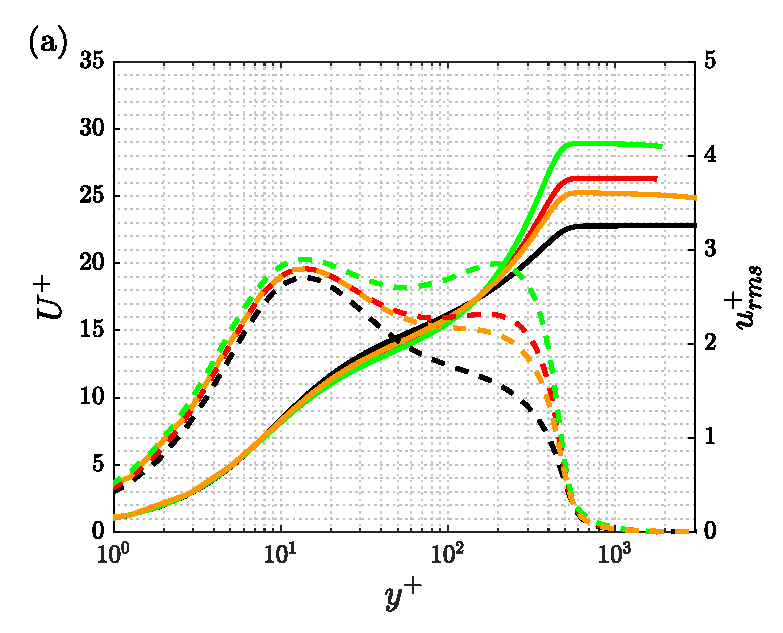
\includegraphics[width=0.49\textwidth]{imgs/stats/U_uu_a.eps}
    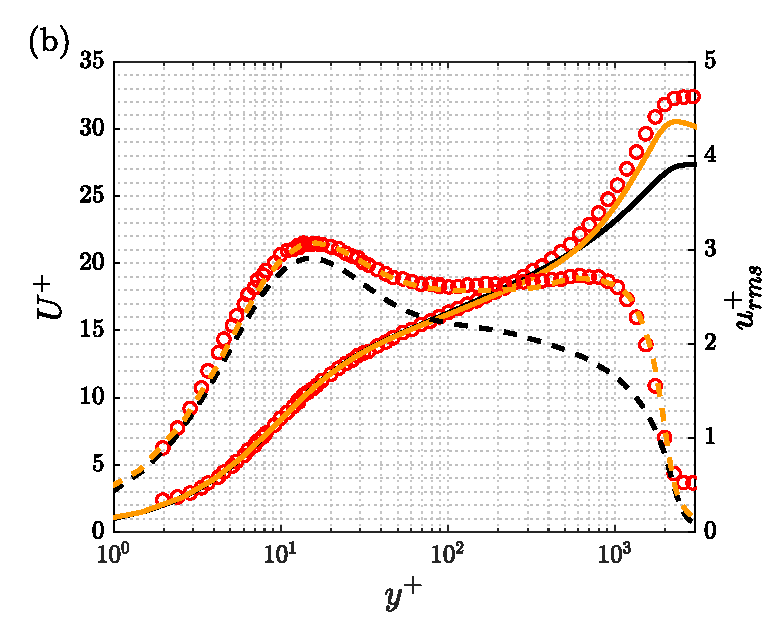
\includegraphics[width=0.49\textwidth]{imgs/stats/U_uu_b.eps}
    \caption{Mean streamwise $U$ (solid lines) and streamwise root mean square $u_{rms}$ or strandard deviation of the streamwise velocity (dashed lines). Wall-normal profiles taken at: (a) $\Rey_{\tau}=500$, (b) $\Rey_{\tau}=2100$. }
    \label{fig:U_uu_cap2}
\end{figure}

\subsection{Friction at the wall, on the friction coefficient $c_f$}

The drag in aerodynamic structures has an important contribution from the friction at the wall, also known as skin friction which is the mean shear stress produced at the wall $\tau_w$, due to the viscous forces.
Instead of $\tau_w$, it is common to look at the friction factor $c_f$ which is a ratio between the friction stresses and the free flow,
\begin{equation}
    c_f = \frac{\rho \tau_w}{1/2 \rho U_e^2} = \frac{2 u_{\tau}^2}{U_e^2} = 2\left( \frac{u_{\tau}}{U_e} \right)^2
\end{equation}
but it can also be seen as an indicator of the friction-velocity with respect to the free-flow velocity.

\begin{figure}
    \centering
    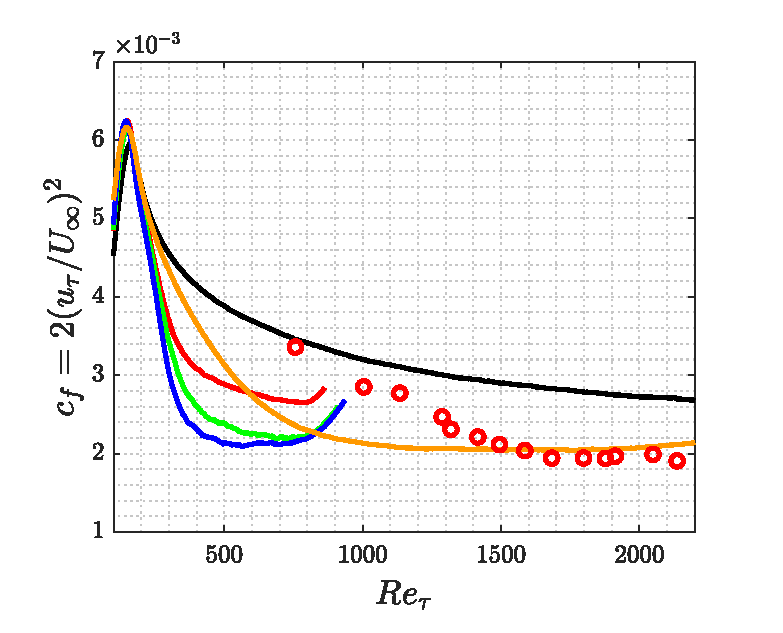
\includegraphics[width=0.85\textwidth]{imgs/stats/cf_Retau.eps}
    \caption{Evolution of the mean friction coefficient $c_f = \pdv{2\overline{\tau_w}}/{U_e^2}$ for ZPG and APG simulations (solid lines) and experiments by \cite{MTL_expSANMIGUEL} (red circles).}
    \label{fig:cap3_evol_cf}
\end{figure}

In Fig.~\ref{fig:cap3_evol_cf} we show the mean friction factor development along the turbulent boundary layers for ZPG and APG simulations and an experimental APG.
It can be seen how for attached flows and near-equilibrium TBLs the trend is positive, decays with the Reynolds number and the value is lower the stronger the APG intensity.
The simulations show an increase for the larger $\Rey_{\tau}$ where the fringe region starts to affect the flow, and this region is not included in the region of interest (ROI) of our database.

The effects of APG on the coefficient $c_f$ are studied through the Renard--Deck (RD) \citep{Renard2016} identity in \textbf{Paper 3} and the Fukagata, Iwamoto \& Kasagi identity (FIK)  \citep{Fukagata2002} in \textbf{Paper 4}.

The FIK decomposition of $c_f$ is adapted to include a join contribution of the pressure gradient and the streamwise convection, looking for a dynamic pressure perspective, instead of treating this antagonizing contributions as a separate entity.

A different approach onto the $c_f$ is that of the RD decomposition, taken from a perspective based on the mean streamwise kinetic energy budget. 
The main contributions to the total $c_f$ are divided in three main terms representing the viscous dissipation, the turbulent kinetic energy production and the spatial growth.
The contribution from the viscous diffusion is mainly located in the inner/near-wall region of the TBL and the influence diminish for stronger APGs, since the influence of the larger scales located in the outer region of the TBL are more energized and its effects on $c_f$ are larger.
The TKE Production close to the wall have a near-wall peak that influences $c_f$, but the influence of APGs produce a strong outer-peak in the outer region.
The spatial growth contribution is further decomposed into three subterms, the main ones are due to the mean convection $\Vec{U}\cdot \nabla\Vec{U}$ (which has a positive contribution across the TBL) and a direct contribution of the pressure-gradient (which has a negative contribution on $c_f$). These terms are more relevant the stronger the APG is and decrease with $\Rey$, and their influence is mostly located in the outer/wake region of the TBL.


\section{Spectral decomposition}
To have a better understanding on the perturbations we can use some mathematical tools such as the decomposition of the spatial-temporal signal using correlations, orthogonal modes, coherent structures, etc.
The use of orthogonal modes allows to decompose the energy of the perturbations into each mode in an unique way, so the sum of the energy contained in all the modes is equivalent to the total energy of the perturbations. 

In signal analysis an orthogonal decomposition which is commonly used is the Fourier decomposition which enables to look for phenomena that repeats with a certain time or spatial frequency. The energy or power associated with each mode is called energy spectra (if the signal is finite such as pulses) or power spectra (if the signal is such as sinusoidal waves, whose domain and energy is not finite, however its power is). Remember that the power is the ratio of the energy over time, where the time goes to infinity (in the case of using temporal series).
Since we are dealing with signals which are periodic in the homogeneous dimension $z$ and are not limited in time, we will use the terminology of power spectra (PS) instead of energy spectra. 
The modes in $z$ have a wavenumber $k_z$ and a wavelength $\lambda_z=2\pi/L_z$ where $L_z$ is the spanwise period of the domain. The same analysis can be applied in time, where we will use $k_t$ and $\lambda_t$.
For a signal $x(t)$, with $X(k_t)$ being its Fourier transform, the power of each mode is $|X(k_z)|^2$, the squared amplitude of the mode. For a perturbation velocity, the power can be calculated as,
\begin{equation}
    PS_{u_i\myprime u_j\myprime}(k_z) = \mathcal{F}(u_i \myprime)  \mathcal{F}^*(u_j \myprime),
    \label{eq:power_sp}
\end{equation}
where $\mathcal{F}()$ is the Fourier transform and $\mathcal{F}^*()$ represents the complex conjugate and the definition has been expanded to include the power spectra of the quantity $\langle u_i\myprime u_j\myprime \rangle_{z}$, also known as cospectra.
Using the properties of the Fourier transform, the multiplication in Fourier space represented in Eq.~\ref{eq:power_sp} represents the Fourier transform of the two-point correlation function $\mathcal{R}_{u_i\myprime, u_j\myprime}(\delta z)=u_i\myprime \star u_j\myprime$, where $\delta z$ is the lag or distance between the two points where we look for the correlation of their velocity perturbations. According to the Wiener--Khinchin theorem, we can calculate the PS through as the Fourier transform of $\mathcal{R}_{u_i\myprime, u_j\myprime}$ or from the power spectra throught the inverse Fourier transform $\mathcal{F}^{-1}()$ we can obtain the two-point correlation function.

Note that for velocity perturbations, since Fourier modes are orthogonal, the sum of the PS for all the modes is equal to the averaged Reynolds stress,
\begin{equation}
    \langle u_i\myprime u_j\myprime \rangle_{z} = \sum_{k_z} PS_{u_i\myprime u_j\myprime}(k_z)
\end{equation}

This step can be performed for each time step and averaged over time to obtain $\langle\langle u_i\myprime u_j\myprime \rangle_{z}\rangle_{t} = \overline{u_i\myprime u_j\myprime}$ or it can also be the result of a 2D spectral decomposition in both time and $z$, where the sum extends to all the spatial and temporal modes.

The PS is useful for discrete systems, and it is the first step when we calculate numerically the spectra of a the Reynolds-stresses. It is also interesting to see how the power spectra is distributed along the wavenumbers or the wavelengths, obtaining a power spectral density (PSD).
The average in time of the PSD in wavenumbers is $\phi_{u_i\myprime u_j\myprime}=\langle PS \rangle_t/\mathrm{d} k_z$ while the average in time PSD in wavelengths is $\psi_{u_i\myprime u_j\myprime}= \langle PS \rangle_t/\mathrm{d} \lambda_z$. Both densities can be linked using $\mathrm{d}(\lambda_z) = \mathrm{d}(2\pi/k_z) = -2\pi\mathrm{d}k_z/k_z^2$:

\begin{equation}
    \psi_{u_i\myprime u_j\myprime} = 
    \frac{ \langle PS_{u_i\myprime u_j\myprime} \rangle_t}{\mathrm{d} \lambda_z} =
    -\frac{ \langle PS_{u_i\myprime u_j\myprime} \rangle_t}{\mathrm{d} k_z} \frac{k_z^2}{2\pi},
\end{equation}
where the minus sign is taking care by inverting the limits of integration to obtain the total RS (small to large wavenumbers is equivalent to integrate from large to small wavelengths).

\begin{equation}
\label{eq:sum_ps}
    \overline{u_i\myprime u_j\myprime} = 
    \int_{k_z=k_0}^{k_z=k_{N}}   \phi_{u_i\myprime u_j\myprime}  ~ \mathrm{d} k_z =
    \int^{\lambda_z = 2\pi/k_0}_{\lambda_z = 2\pi/k_{N}}  \psi_{u_i\myprime u_j\myprime}  ~ \mathrm{d} \lambda_z
\end{equation}

In Fig.~\ref{fig:PS_PSD} we show for a ZPG TBL, different representations of the PSD of $\overline{u\myprime u\myprime}$ where the image with the black contours represent a streamwise profile at $\Rey_{\tau}=2000$ while the red contours are taken at a position where $\Rey_{\tau}=500$.

\begin{figure}[h!]
\centering
% \captionsetup{width=0.99 \textwidth}
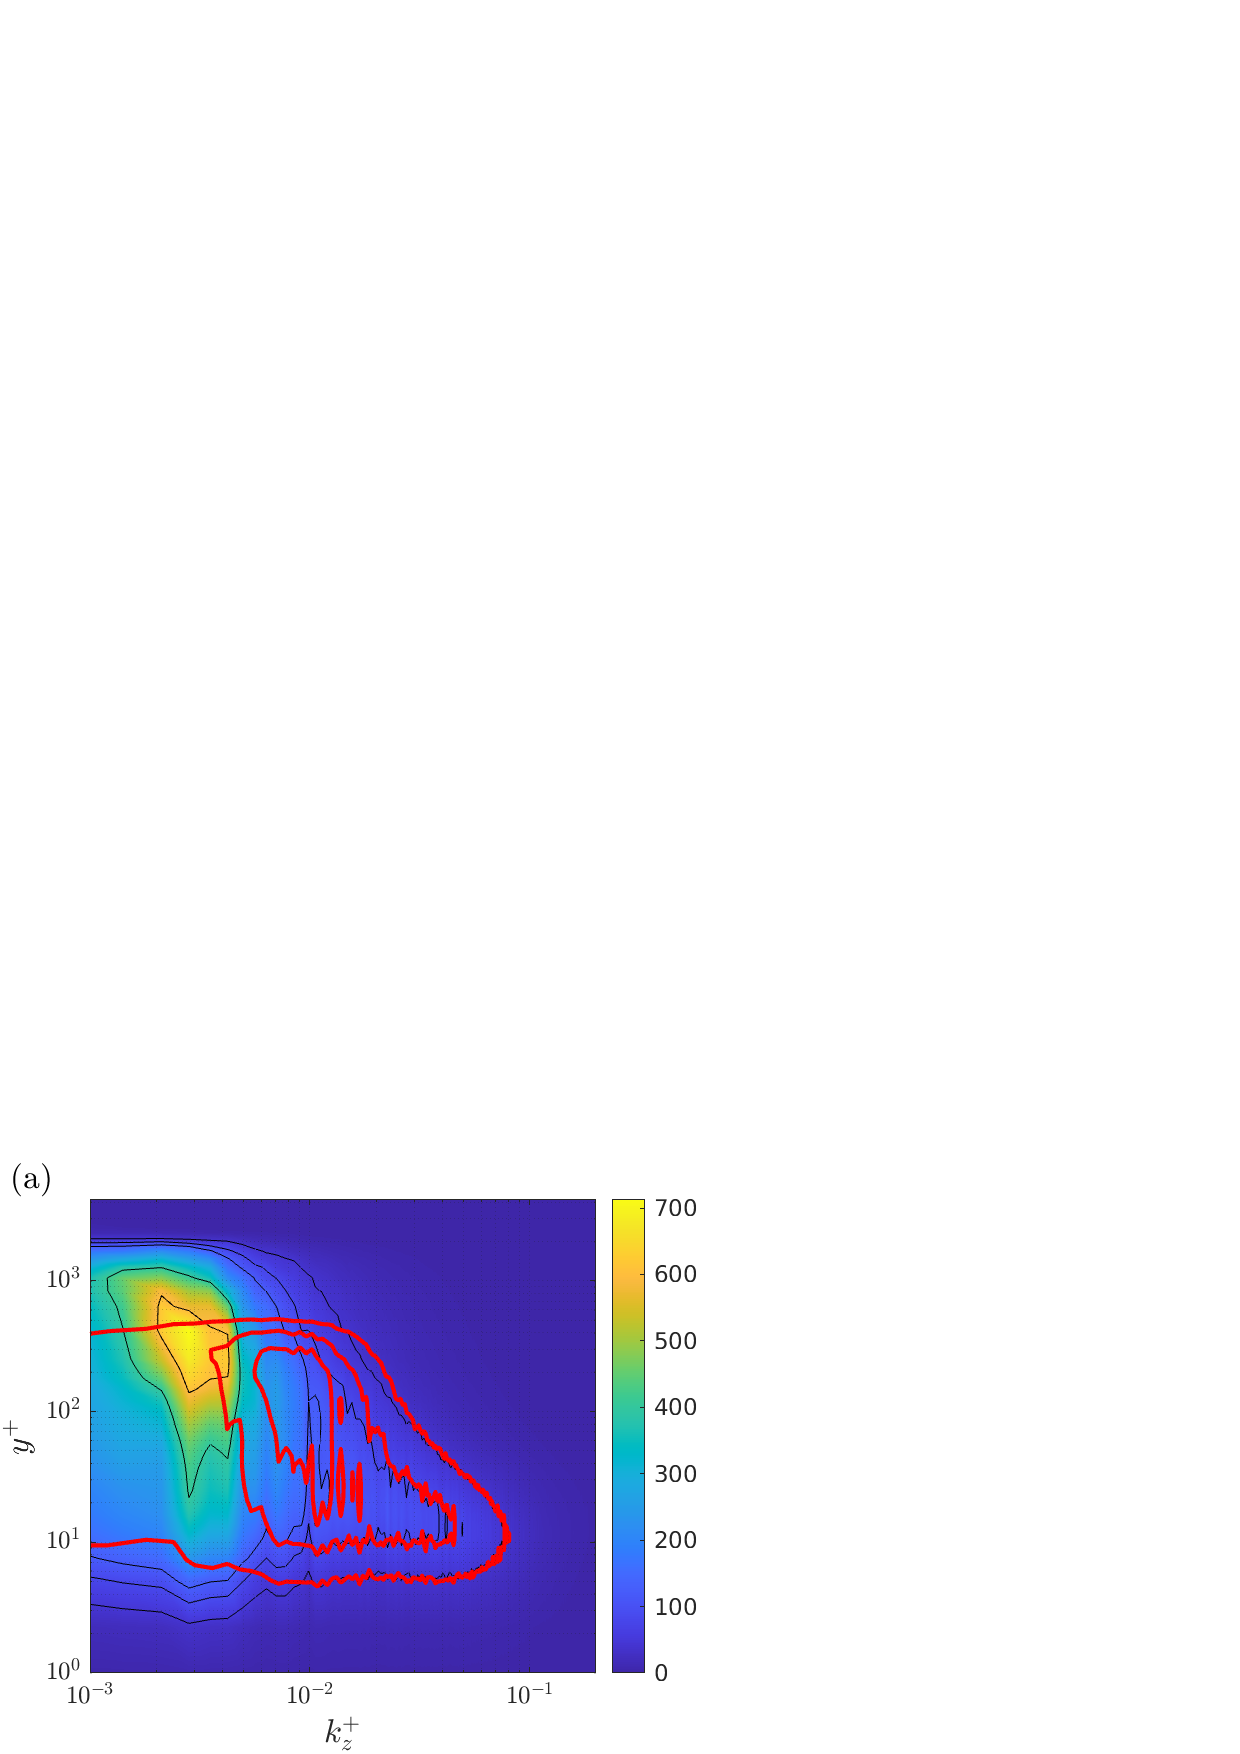
\includegraphics[width=0.32\textwidth ]{imgs/spec/ZPG_Ret_500_2000_PSdkz_kz_ltau_y_ltau.jpg}
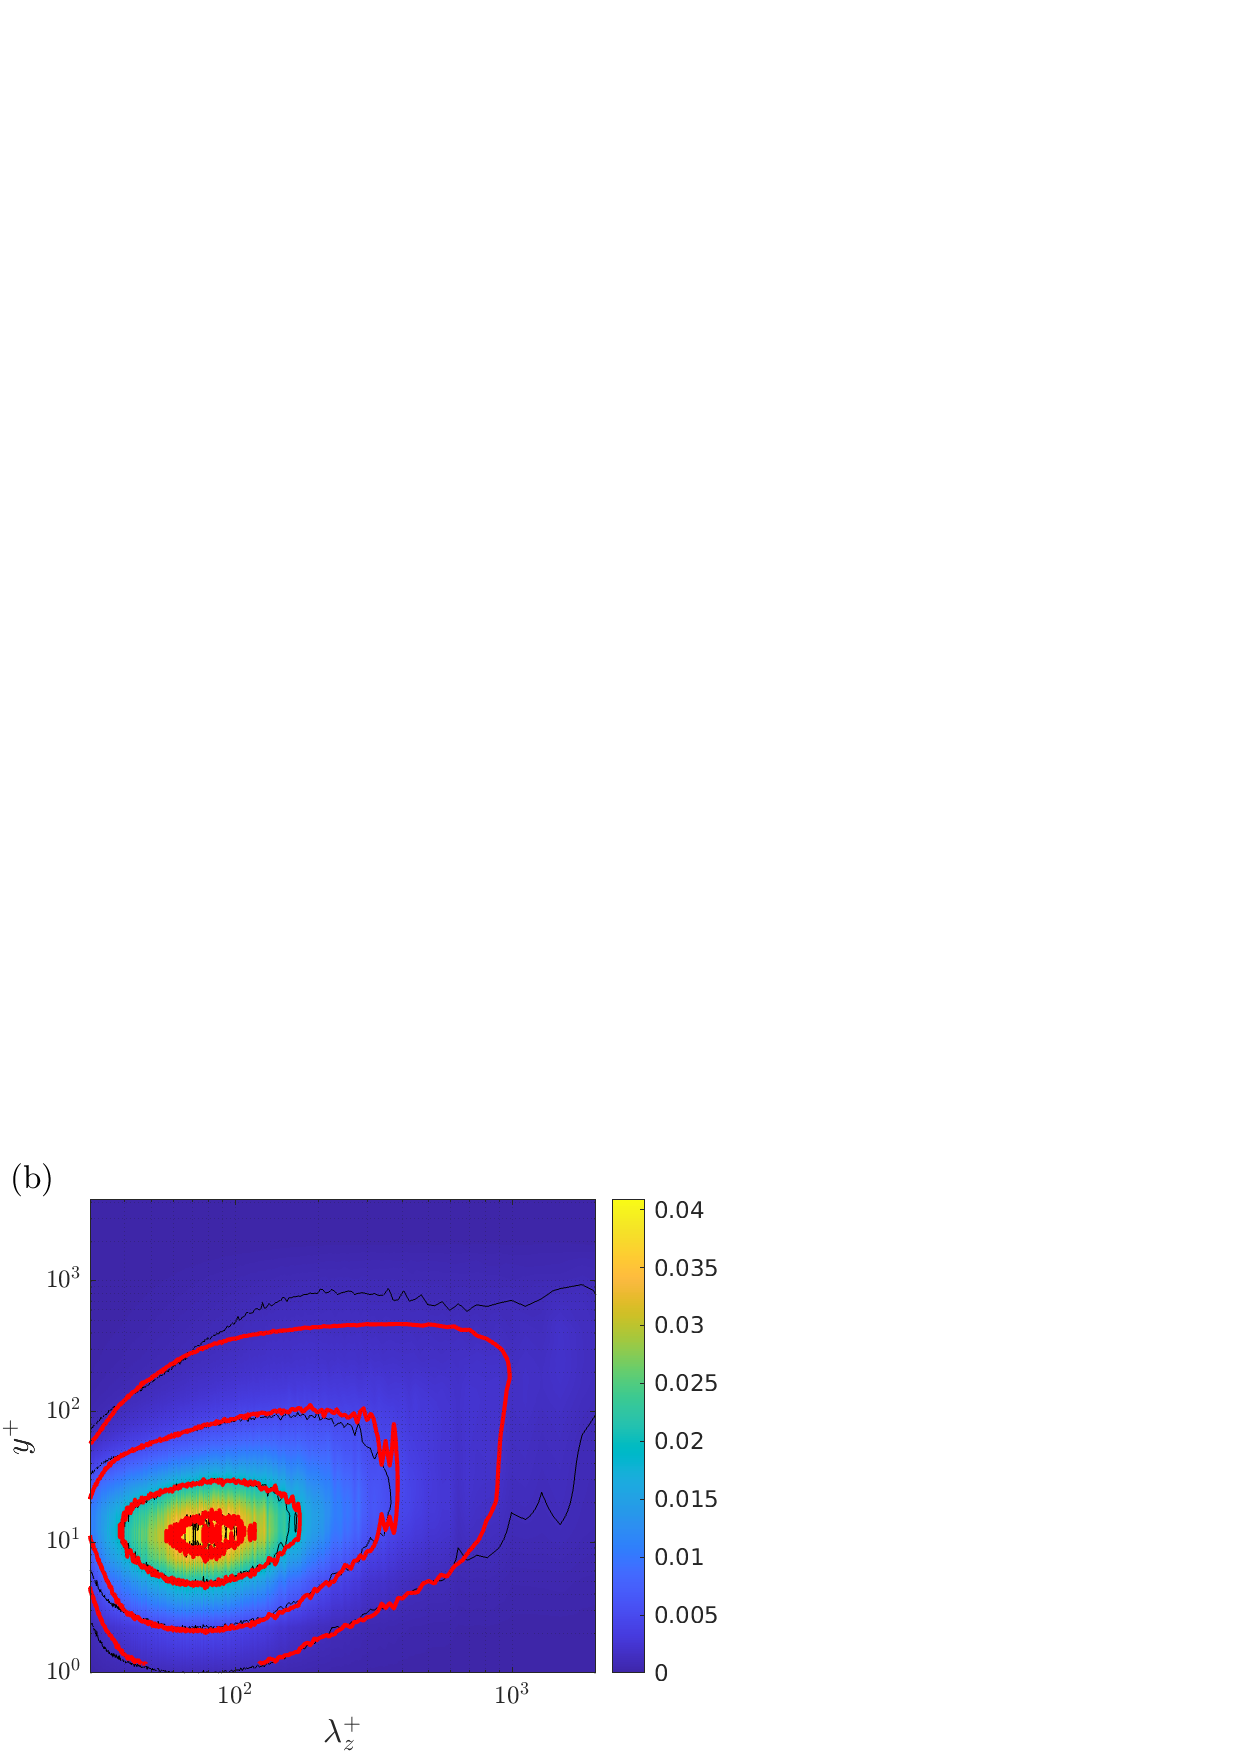
\includegraphics[width=0.32\textwidth]{imgs/spec/ZPG_Ret_500_2000_PSdlambdaz_lambdaz_ltau_y_ltau.jpg}
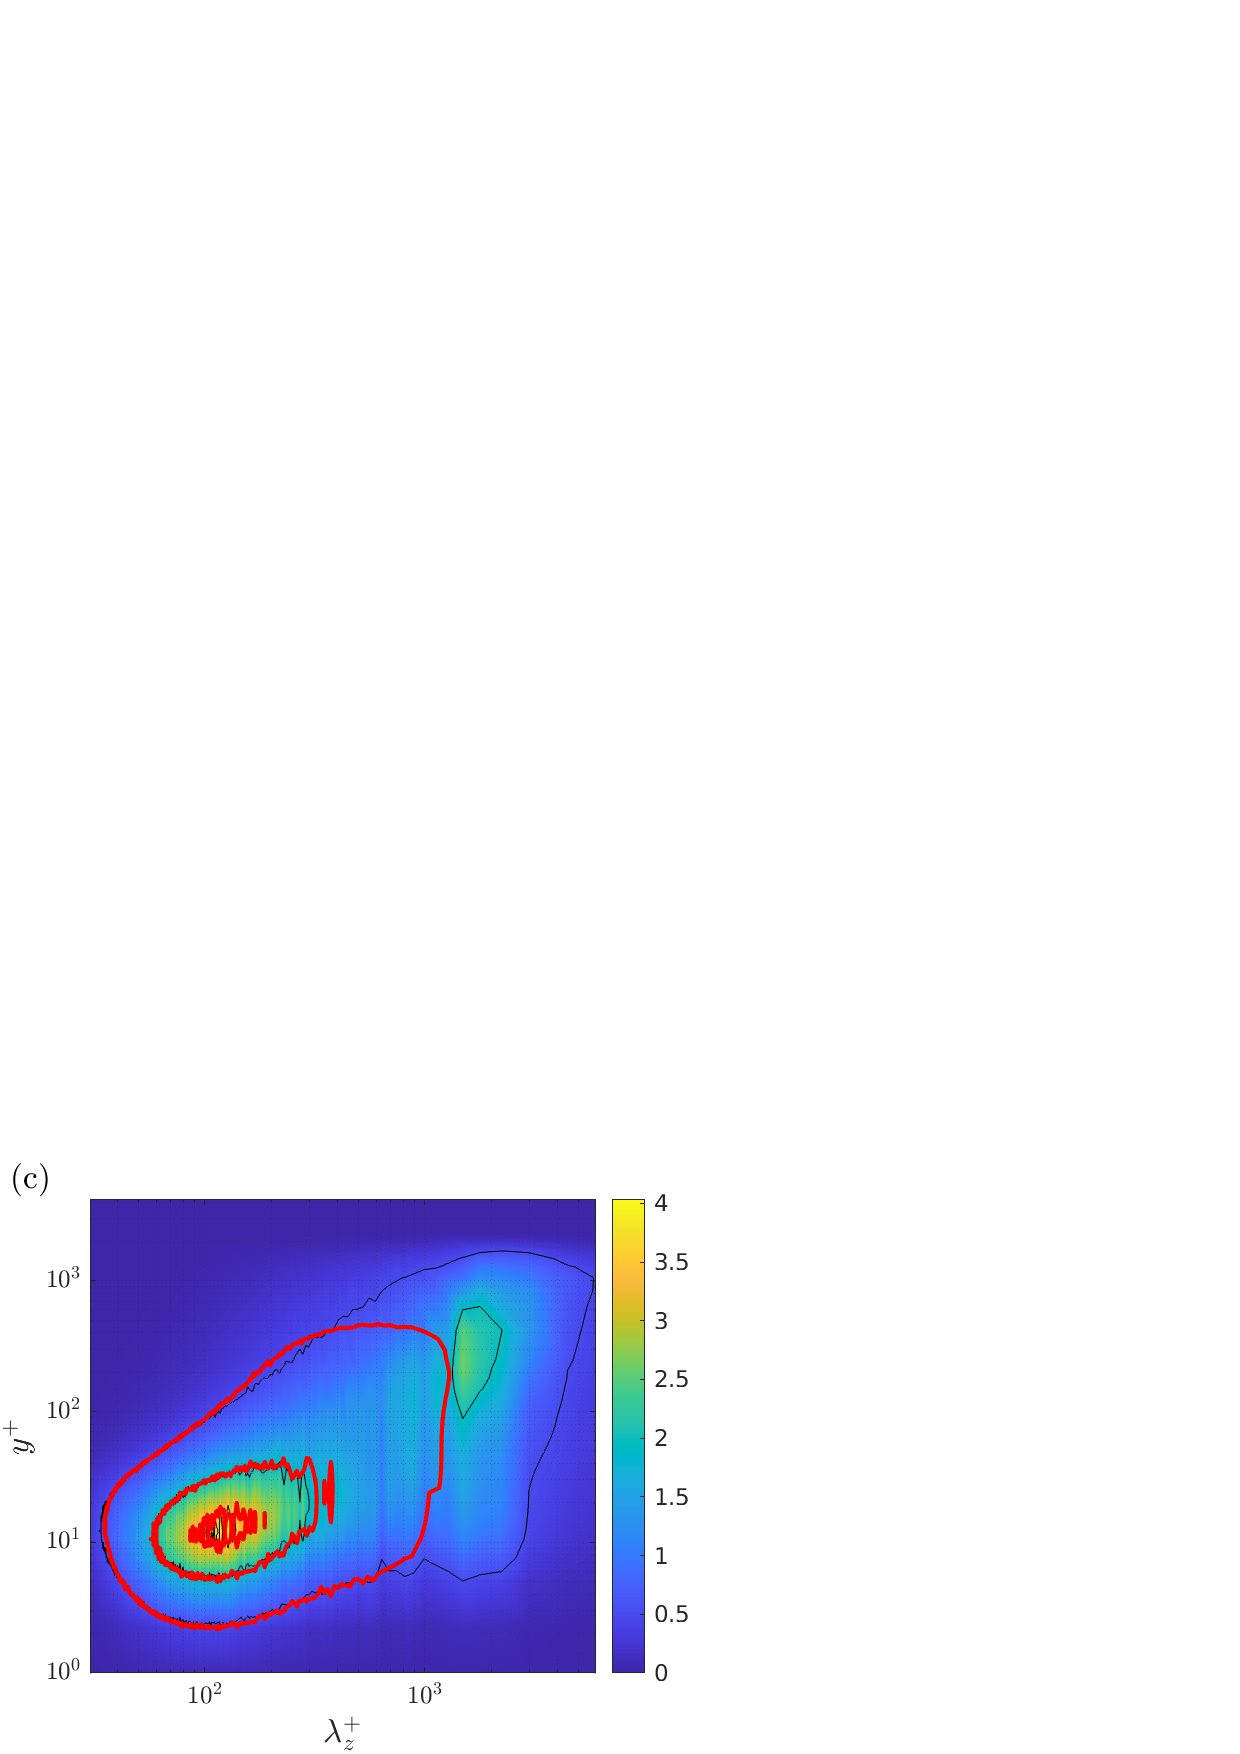
\includegraphics[width=0.32\textwidth]{imgs/spec/ZPG_Ret_500_2000_kPSdkz_lambdaz_ltau_y_ltau.jpg}
\caption{ \label{fig:PS_PSD} Spanwise spectra of the streamwise Reynolds stress $\overline{uu}(y)$. (a) Power spectral density $\phi_{u\myprime u\myprime}(y,k_z)$; (b) Power spectral density $\psi_{u\myprime u\myprime}(y,\lambda_z)$; (c) premultiplied power spectral density $k_z\phi_{u\myprime u\myprime}$. Wavenumbers, wavelengths, wall-normal position and power spectra scaled in viscous units.}
\end{figure}
% contours: Retau 2000: [40 80  120 400 600]; [0.001 0.005 0.02 0.035 0.04] ;  [ 0.5 2 3.5]; 
% contours: Retau  500: [40 80  120        ]; [0.001 0.005 0.02 0.035 0.04] ;  [ 0.5 2 3.5]; 

The PS and the PSD in the wavenumbers $\phi_{u\myprime u\myprime}(y,k_z)$ present the same features as in Fig.~\ref{fig:PS_PSD}(a), since $dk_z$ or $dk_z^+$ are constant factors that does not vary with the wavenumbers. It shows a high content of power/energy of structures with a very low wavenumber which are very wide. It is possible to see similarities in the contours at different Reynolds numbers (red and black lines) in the region of high wavenumbers (small scales), although the energetic level is very low compared to that of the low wavenumbers (large scales).
The PSD in wavelengths $\phi_{u\myprime u\myprime}(y,\lambda_z)$ is represented in Fig.~\ref{fig:PS_PSD}(b) and it focuses on the small scales. It shows that the density of power/energy in the small scales (short wavelengths) is very similar at different Reynolds numbers and larger than the PSD of the wider scales (large $\lambda_z^+$). 
From Fig.~\ref{fig:PS_PSD}(a) and (b) we see that the small scales have a small content of the total RS energy, but their small size make the density in waveleghts to be very concentrated, while for the wider scales is the opposite, the energy they contain is very large, but their big size make the PSD to be very low or disperse.
If we write both PSD as a function of $\phi_{u\myprime u\myprime}$, in Fig.~\ref{fig:PS_PSD}(a) we show $\phi_{u\myprime u\myprime}$ while in Fig.~\ref{fig:PS_PSD}(b) it would be $k_z^2 \phi_{u\myprime u\myprime}$, the premultiplication factor $k_z^2$ is responsible to augment the effects of the small scales while diminishing the effects of the large scales. Fig.~\ref{fig:PS_PSD}(c) shows $k_z \phi_{u\myprime u\myprime}$, whose effect equilibrates the effect of the large and small scales obtaining a better visualization of both scales.

The premultiplied PSD $k_z \phi_{u\myprime u\myprime}$ is widely used and it has a geometrical explanation.
Since the range of energetic scales is so large that we observe very small scales close to the wall and very large scales of the size of $\delta_99$, the use of logarithmic axis helps to expand the region of small $\lambda_z$ and the region close to the wall.
If we use logarithms in the definition of wavelength, $ \mathrm{ln}(\lambda_s) = \mathrm{ln}(2\pi) - \mathrm{ln}(k_z)$, and apply the differential, $\mathrm{d}(\mathrm{ln} \lambda_z) = -\mathrm{d}(\mathrm{ln} k_z)$, and together with $\mathrm{d}k_z = k_z \mathrm{d}(\mathrm{ln} k_z)$ can be substituted in Eq.~\ref{eq:sum_ps} to obtain:
\begin{equation}
    \overline{u_i\myprime u_j\myprime} = 
    \int_{k_0}^{k_{N}}   \phi_{u_i\myprime u_j\myprime}  ~ \mathrm{d} k_z = 
    \int_{k_0}^{k_{N}}   \phi_{u_i\myprime u_j\myprime} k_z  ~ \mathrm{d}( \mathrm{ln} k_z) = 
    \int^{\lambda_0}_{\lambda_{N}}   \phi_{u_i\myprime u_j\myprime} k_z ~ \mathrm{d}( \mathrm{ln} \lambda_z).
\end{equation}

The premultiplication by $k_z$ can be seen here as a factor to visualize a corrected area after scaling the axis with a logarithmic scale.
From here on the PSD will always be represented in its premultiplied form $k_z\phi$ to have a clear visualization of the effects of large and small scales at the same time.

\subsection{Wide scales in turbulence. Channel Flows}
It has been seen that the big scales contains a large part of the turbulent energy, although the density spectral density is low.
When we model the turbulent flow, the size of the domain imposes a limit on the size of the scales that can be simulated. In a periodic domain, the largest scale corresponds to $L_x$ and the wider scale to $L_z$. Bigger scales will be seen as infinit in size because of the periodicity, and the spectral energy will be stored in the zero-wavenumbers.

The energy contained in the zero-wavenumbers is affected by the averaging.

If the size of the domain is not large or wide enough, the bigger turbulent scales will not be able to be captured and the energetic spectrum will not be correct, affecting the total statistics such as the Reynolds stresses and the mean velocity profiles.
Many analysis on the size of the domain has been performed on canonical turbulent channel flows for it simplicity.
\highlight{Minimal channels are those small domains that assure }
On the other way, the largest scales in channel flows where looked for in \highlight{CITAR ADRIAN que descubrieron bla bla}.
The study on the wider scales was based on two-point correlations, but no other study similar to \highlight{CITAR ADRIAN} was performed in the spanwise direction.

To have a better understunding of the wide scales obtained in APG TBLs and the effects of the domain size, we decided to study first the effect on wide-channels.
Three simulations were performed of turbulent channel flows at $\Rey_{\tau} = 550 $ under similar conditions, with the only excemption the width of their domains which was doubled from one channel to another as it can be seen in Tab.~\ref{tab:param_WC_cap2}.
 
\begin{table}
    \begin{center}
    \def~{\hphantom{0}}
    \begin{tabular}{ l r  r  r  r }
    Case  & $L_x/h$ & $L_y/h$ & $L_z/h$ &  Colour     \\[3pt]
    C1    & 8$\pi$  &    2    & 4$\pi$  &  \redline   \\
    C2    & 8$\pi$  &    2    & 8$\pi$  &  \redline   \\
    C3    & 8$\pi$  &    2    & 16$\pi$ &  \redline   \\
    \end{tabular}
    \caption{Parameters of the channel flows simulations. The reference length $h$ corresponds to half the channel's height. The box size is $(L_x/h, L_y/h , L_z/h)$.}
    \label{tab:param_WC_cap2}
    \end{center}
\end{table}

\highlight{The contours of the PS or the spectral density $\phi(k_Z, y)$ are not closed for the largest scales when $k_z \rightarrow 0$. The largest scale captured by Fourier analysis corresponds to $k_Z=(2\pi)/L_z$ or $L_z$, and $k_z=0$ corresponds to an averaged energy. 
The property where the integral of the PSD equals the RS component includes the energy contained in the wavenumber $k_z=0$. The premultiplication by $k_z$ automatically cancels that energy, making it inappropriate to use premultiplied spectra for integral analysis. 
Then this question arises, ``is it possible to have a domain $L_z$ where the largest Fourier scales $\lambda_z=\{L_z, L_z/2, ... \}$ does not contain spectral energy, therefore the contours are closed?''.
And the answer is that it depends on the averaging that we use. This answer will be explained using the Reynolds-average decomposition that we have introduced previously, and apply it to the component $u$.}
With $PS_T$ we denote the power spectra of the total velocity $u$, and the energy contained in the wavenumber $k_z$ corresponds to the average in $z$.


\begin{equation}
    PS_T = \mathcal{F}(u)\mathcal{F}^*(u) = \mathcal{F}(U)\mathcal{F}^*(U) + \mathcal{F}(u\myprime)\mathcal{F}^*(u\myprime) + \mathcal{F}(U)\mathcal{F}^*(u\myprime) + \mathcal{F}(u\myprime)\mathcal{F}^*(U)  
\end{equation}

\begin{flalign}
    % \label{eq:intsc_3term_small}
     PS_T =& \mathcal{F}(u)\mathcal{F}^*(u) &&\\\nonumber
     =&  \mathcal{F}(U)\mathcal{F}^*(U) + \mathcal{F}(u\myprime)\mathcal{F}^*(u\myprime) + \mathcal{F}(U)\mathcal{F}^*(u\myprime) + \mathcal{F}(u\myprime)\mathcal{F}^*(U) &&\\\nonumber
     =&  UU + \mathcal{F}(u\myprime)\mathcal{F}^*(u\myprime) + U(\mathcal{F}(u\myprime) + \mathcal{F}^*(u\myprime)) &&\\\nonumber
\end{flalign}  
\rev{and the last term vanishes when the time average is performed?}

\begin{equation}
\begin{split}
    % \label{eq:intsc_3term_small}
     PS(k_z=0,t) = \langle u\myprime \rangle_z \langle u\myprime \rangle_z  (t) \\
     \langle PS(k_z=0) \rangle_t = \langle (\langle u\myprime \rangle_z)^2 \rangle_t > 0,
\end{split}
\end{equation}
since by definition, $U$ and $u\myprime$ are chosen as a constant and a fluctuation based on the total average $\overline{( \cdot )} = \langle \langle ( \cdot ) \rangle_z \rangle_t$, and $\overline{u\myprime}=0$, but $ \langle u\myprime \rangle_z \neq 0$.

Therefore, the energy contained in $k_z=0$ can not be 0, but it is somehow a result of the average used for the decomposition.
What can be study is how the energy contained in $k_z=0$ changes with $L_z$, and even more relevant from the physical point of view is how much is the energy contained in the first wavenumbers or the largest scales $\lambda_z=L_z, L_z/2, L_z/3,...$.


\subsection{Spectral results on APG}

In \textbf{Paper 1} the 1D spanwise spectra and the 2D spanwise and temporal spectra of the APG TBL where shown and compared to those of a ZPG TBL \citep{EAmorZPG}. By using percentage contours it was possible to show a similar behaviour in the mild APG and the ZPG simulations at different Reynolds numbers in the small-scale energy region close to the wall around an spectral near-wall peak or spectral inner peak (sIP) at $y^+\approx 15$ and $\lambda_z^+\approx 120$. Another region with similar shape is in the wake region with an spectral outer peak that seemed to scale with the Reynolds number.
Another region is that of small-scale energy in the wake region, which is only present in the APG simulation and not in the ZPG case.

\begin{figure}[h!]
\centering
% \captionsetup{width=0.99 \textwidth}
\includegraphics[width=0.48\textwidth]{ZPG_uu.jpg}
\includegraphics[width=0.48\textwidth]{APG_uu.jpg}
% 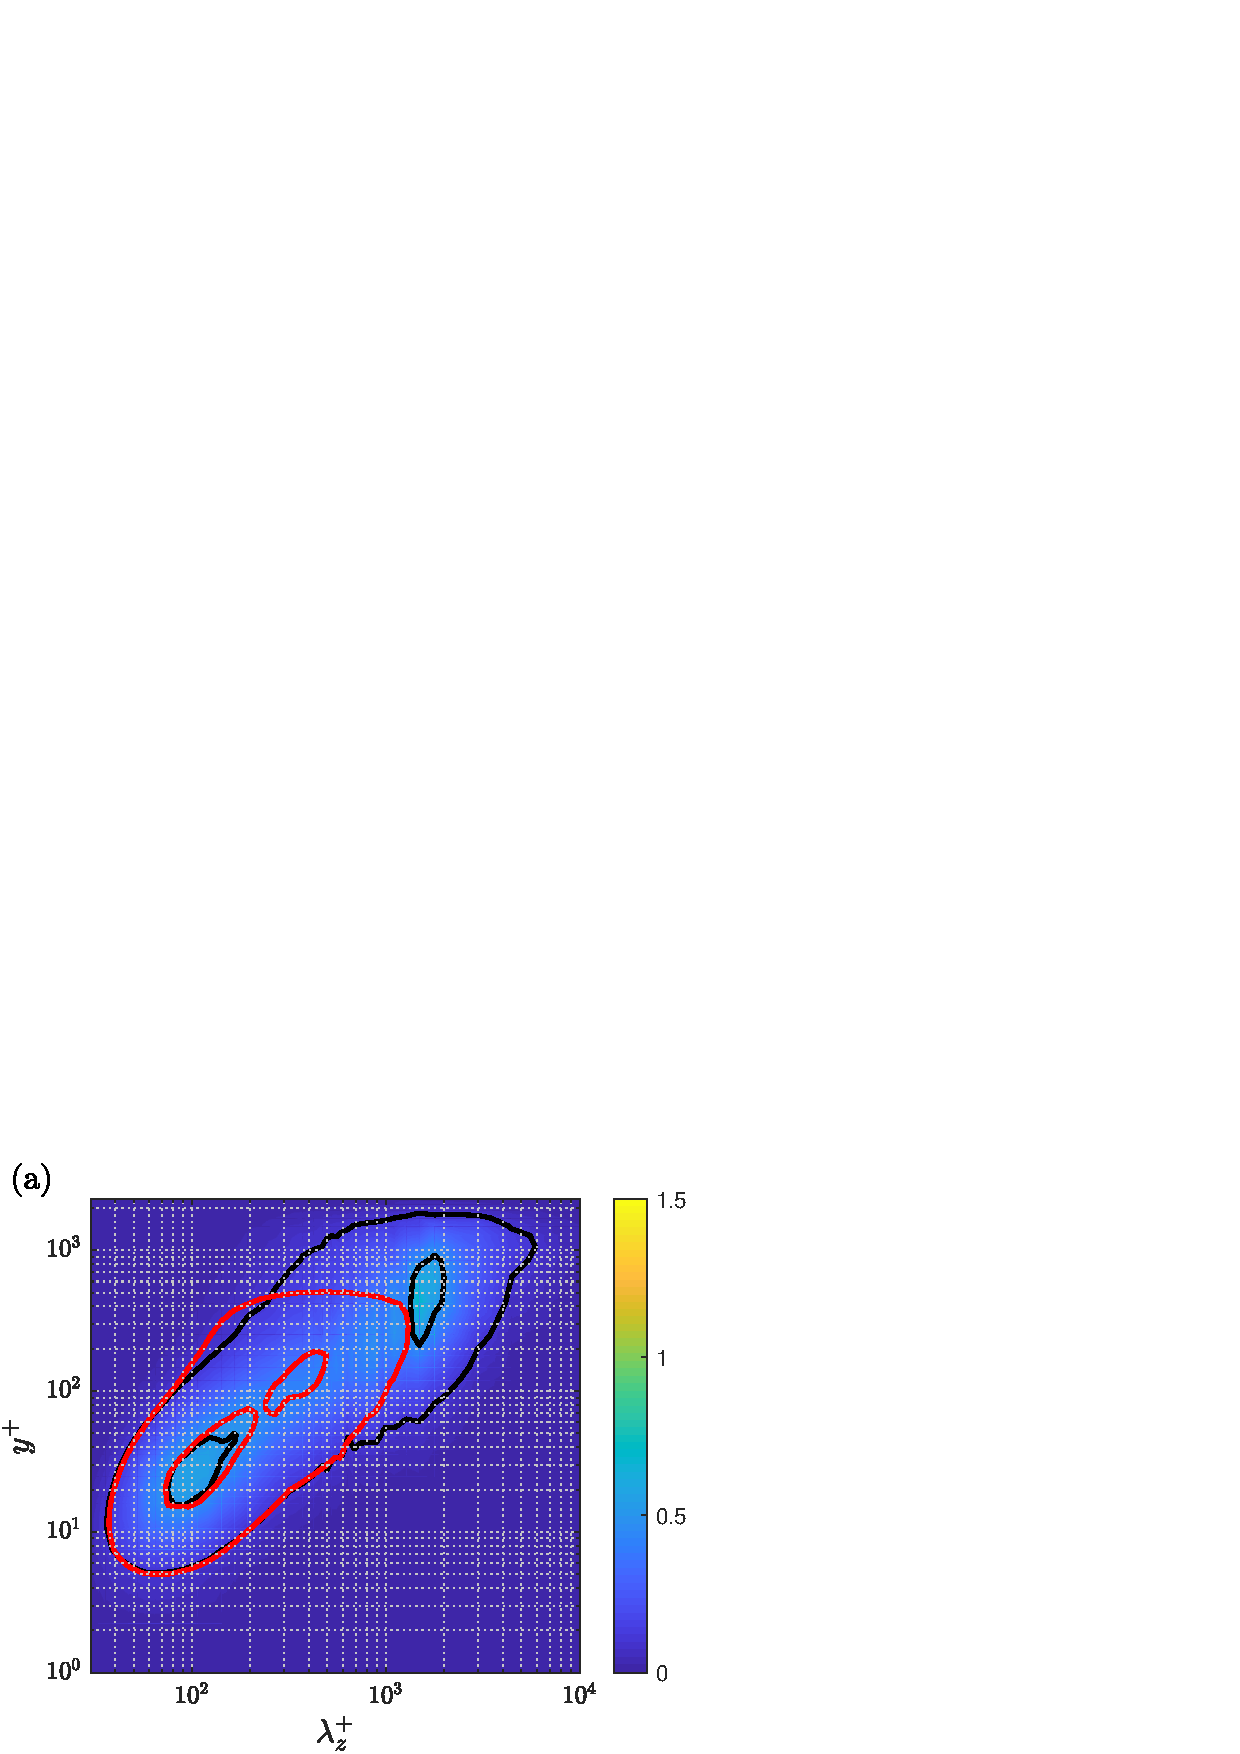
\includegraphics[width=0.48\textwidth]{ZPG_uv.jpg}
% 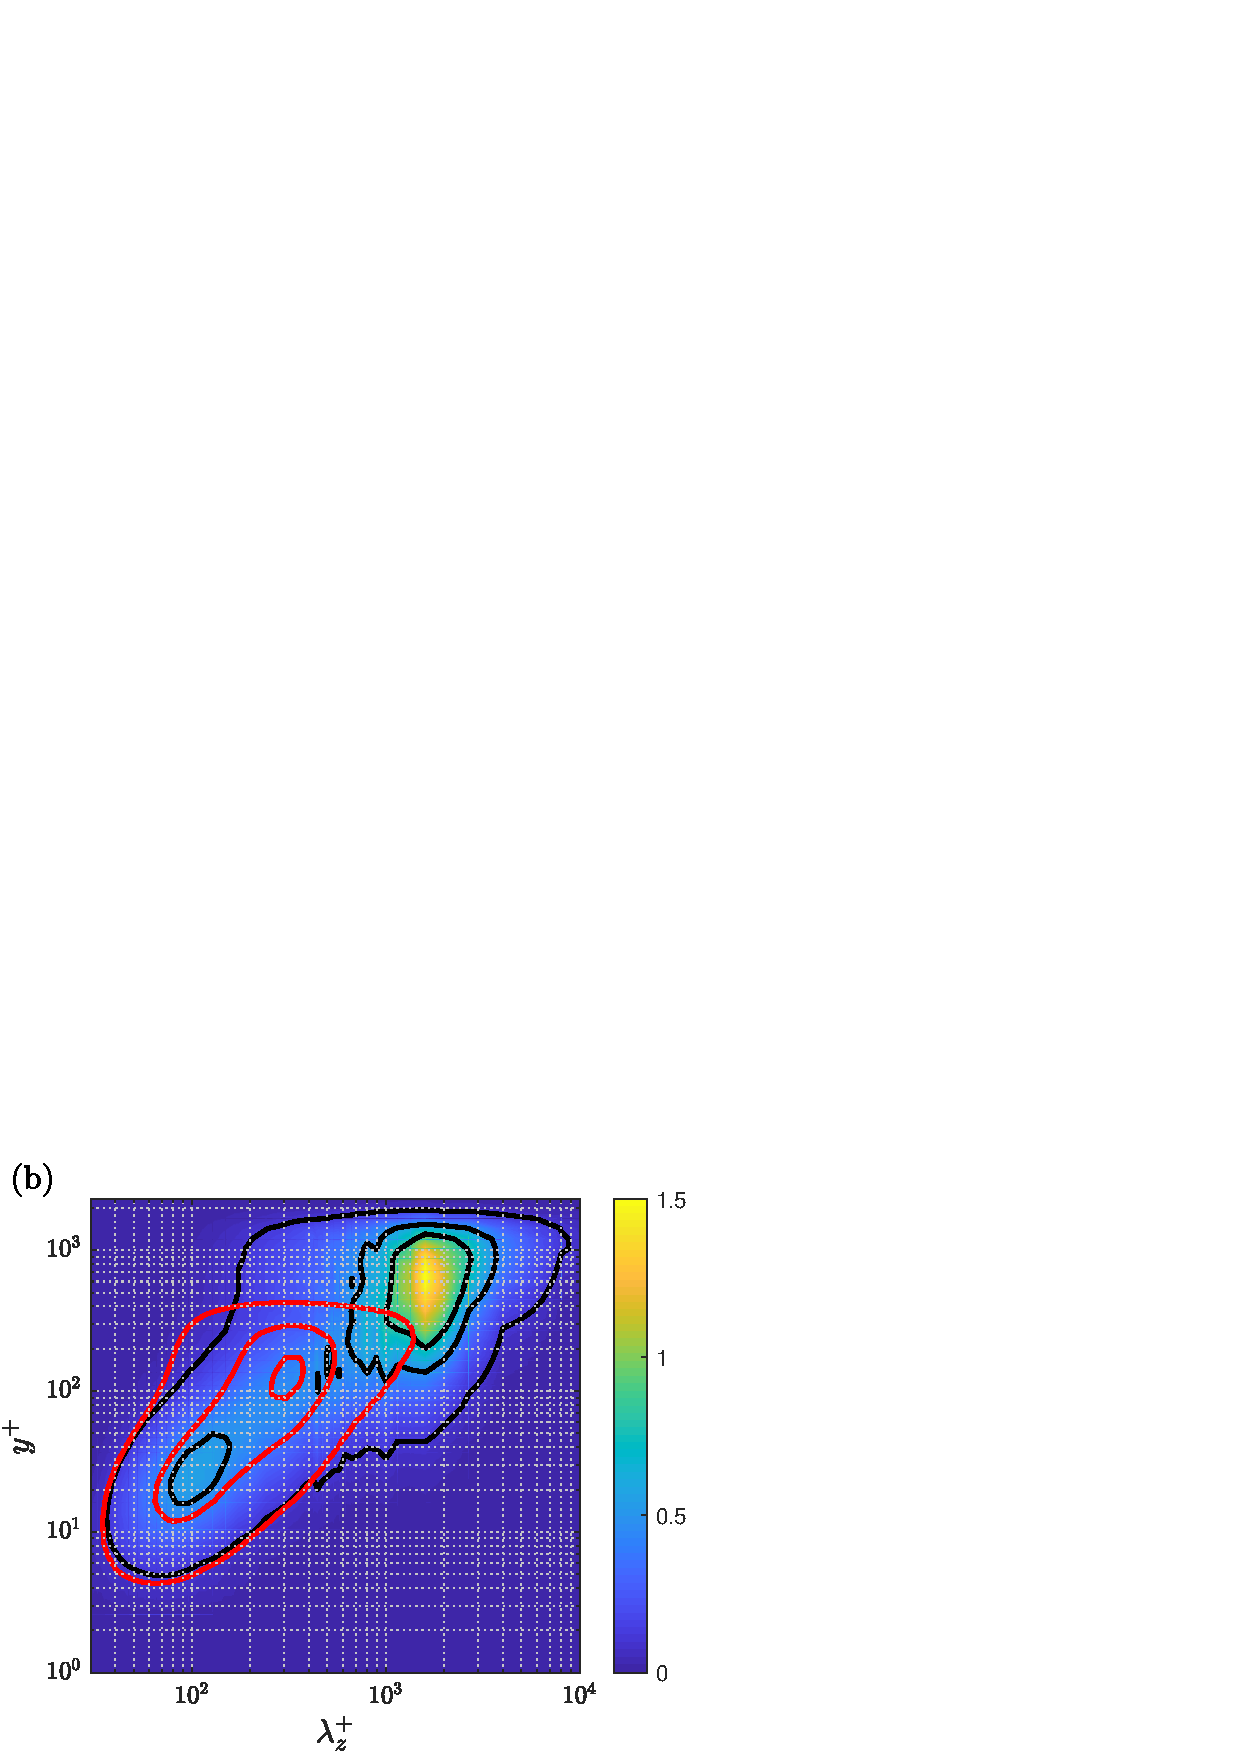
\includegraphics[width=0.48\textwidth]{APG_uv.jpg}
\caption{ \label{fig:ZPG_APG_Ret_500_2000_uu} Premultiplied spectrum $k_z\phi_{uu}$ for (a)ZPG and (b)b1.4 simulations. Red contours at $\Rey_{\tau}=500$ and background and black contour are at a positions $\Rey_{\tau}=2000$. }
\end{figure}

\begin{figure}[h!]
\centering
% \captionsetup{width=0.99 \textwidth}
% \includegraphics[width=0.48\textwidth]{ZPG_uu.jpg}
% \includegraphics[width=0.48\textwidth]{APG_uu.jpg}
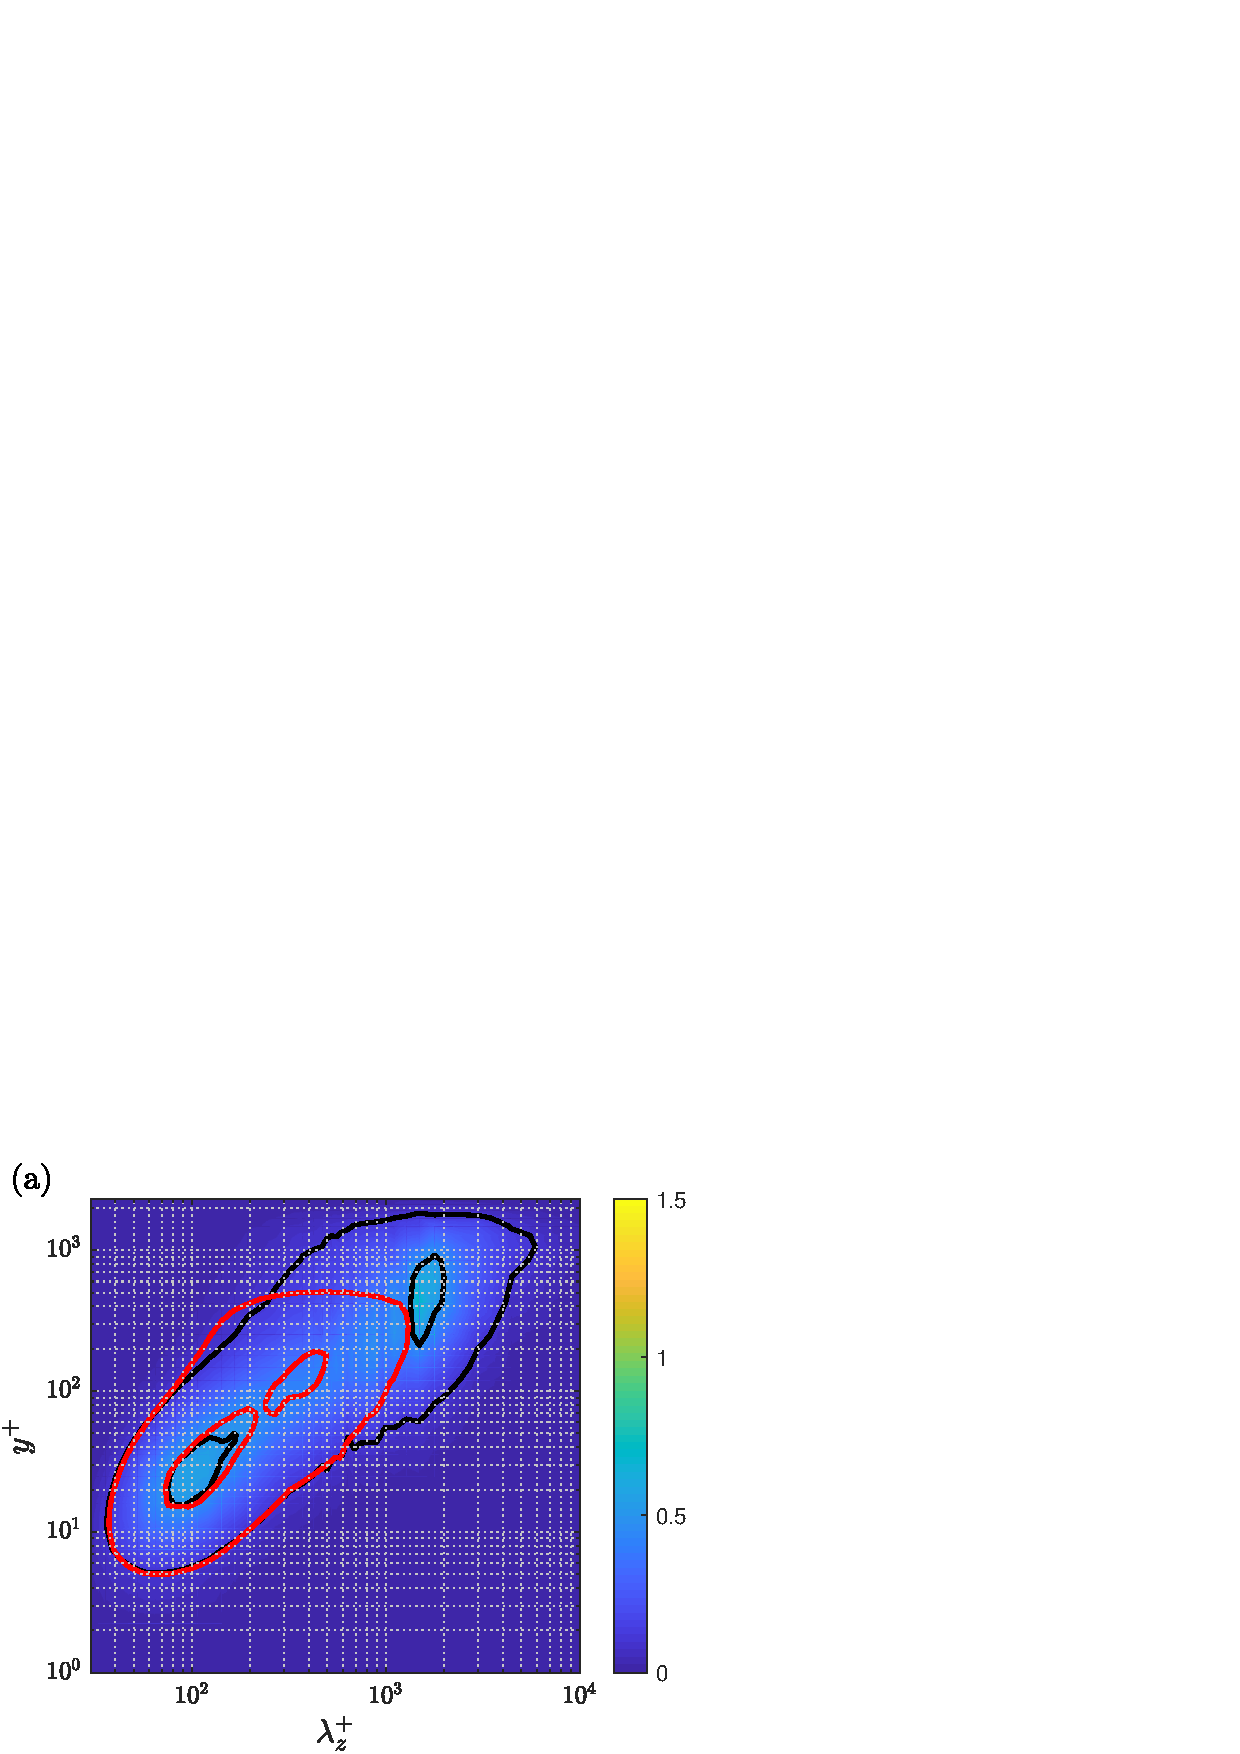
\includegraphics[width=0.48\textwidth]{ZPG_uv.jpg}
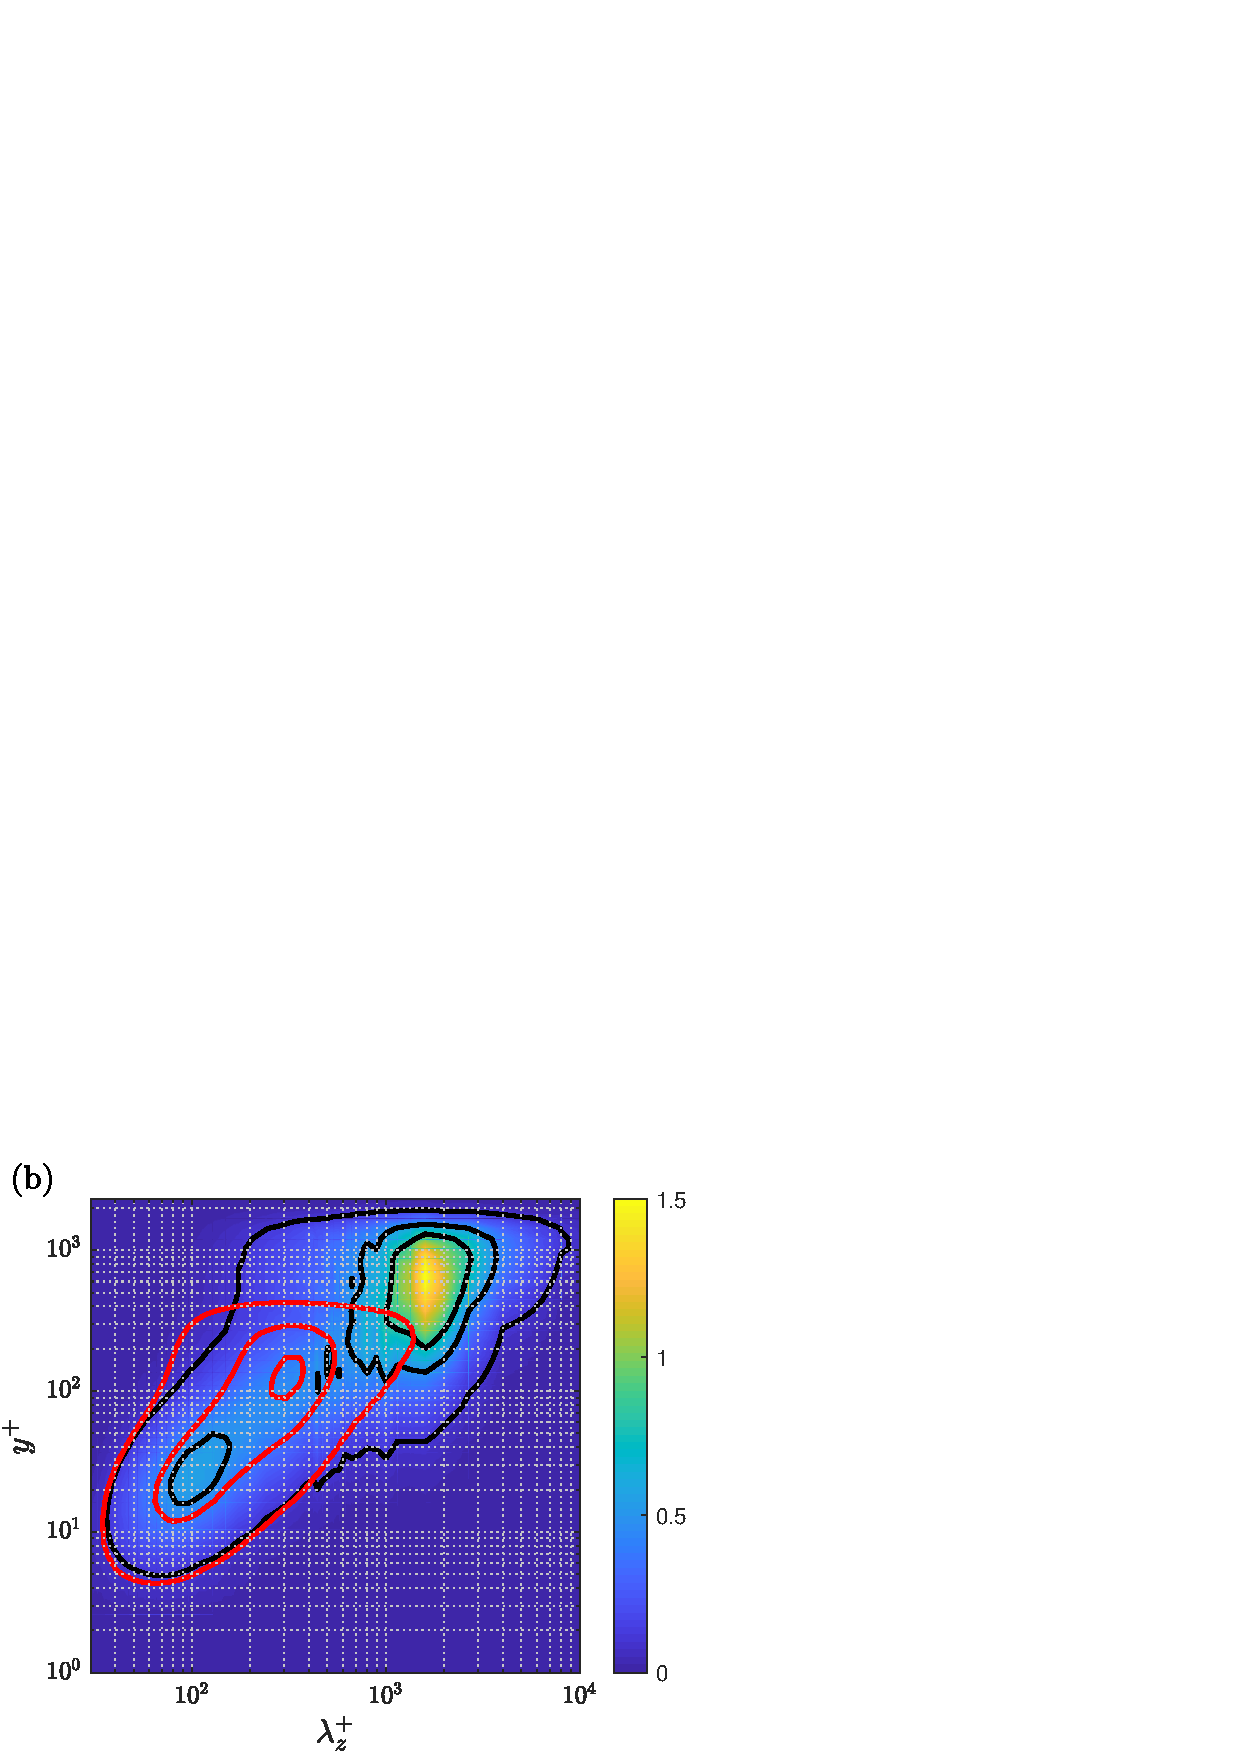
\includegraphics[width=0.48\textwidth]{APG_uv.jpg}
\caption{ \label{fig:ZPG_APG_Ret_500_2000_uv} Premultiplied spectrum $k_z\phi_{uu}$ and $|k_z\phi_{uv}|$ for (a)ZPG and (b)b1.4 simulations. Red contours at $\Rey_{\tau}=500$ and background and black contour are at a positions $\Rey_{\tau}=2000$. }
\end{figure}

The spectra shows a similar region of small-scale energy close to the wall which is responsible of the near-wall peak the RS $\overline{u\myprime u\myprime}$. The effects of $\Rey$ and $\beta$ increase the value of $\overline{u\myprime u\myprime}_{IP}^+$, even if the most of the spectra is similar for APG and ZPG at different Reynolds numbers.
The outer-spectral peak in $k_z\phi_{uu}$ is also responsible of most of the energy contained in the ZPG in the wake region, and increasing $\beta$ it increases the energy to the point of growing the outer peak in $\overline{u\myprime u\myprime}_{OP}^+$. This behaviour is similar in the other components of the RS tensor, where at higher $\Rey$ numbers there are larger and energetic scales acting on the wake region and influencing all across the TBL.

\subsection{Scaling of APG spectrum}

In \textbf{Paper 2} we try to understand the trends of the inner and outer peaks in $\overline{u\myprime u\myprime}$ shown in \textbf{Paper 1}. Why the inner scaled inner-peak grows with the Reynolds numbers and with the APG effects. Is it still correct to use viscous scaling?. 
We perform a scaling analysis of the different energetic scales of the power spectral density for both ZPG and APG simulations and at different Reynolds numbers.
First we start from the features observed in $k_z\phi_{u\myprime u\myprime}$ which are an spectral near-wall/inner peak (sIP) and an spectral outer peak (sOP). The data is scanned to look for the maxima at a certain wall-normal position and the maxima at a certain frequency. Since $k_z\phi_{u\myprime u\myprime}$ is saved in a rectangular matrix, it is equivalent to obtain the maxima along columns and the maxima along rows.
At high Reynolds number the separation of scales even in ZPG TBLs, allows to distinguish clearly the presence of 2 maximal points for $\Rey_{\tau}>500$. Other techniques could be used to detect the local maxima, but this method was obtaining satisfactory results, specially the values of $f(y)=max(k_z\phi(k_z, y))_{k_z}$ since that function presents less noise and it is shown in \highlight{ Fig.~\ref{fig:scaling_OP} figura de los escalados de los picos} that once the Reynolds number is enough to have separation of scales, the outer peak clearly separates in the wall-normal direction from the spectral near-wall peak.
Once sIP and sOP are located in $k_z\phi(k_z, y)$, (usually we represent with $\lambda_z$), we try the inner and outer length scalings used in \textbf{Paper 1} to scale $\overline{u\myprime u\myprime}(y)$.
It is shown that the viscous length $\ell_{\tau}$ scales the size of the spanwise scales of the sIP $\lambda_{z, sIP}^+$ as well as the wall-normal position $y^+_{sIP}$.
The same method is used for the spectral outer peak. The outer scales $\delta^*$ and $\delta_{99}$ were used to scale independently the wall-normal location $y_{sOP}$ and the size of the scales $\lambda_{z, sOP}$.
In previous studies such as \cite{Kitsios2017} the $\delta^*$ scaling was successful for the $y_{OP}$ as well as for $y_{sOP}$ at much higher $\beta$, however, $\lambda_z$ was also scaled with the same scaling.
In \cite{tanarro_2020}, the outer scaling was performed with $\delta_{99}$ for both $y$ and $\lambda_z$, and the values of $\lambda_{z,sOP}$ were better collapsed than using $\delta^*$ as in \cite{Kitsios2017}.
Taking into account this previous studies, we allowed $y$ and $\lambda_z$ to have different length scalings, and found the optimal collapse of the region around the spectral outer peak using $y/\delta^*$ and $\lambda_z/\delta_{99}$.

Once we obtained the scalings for the wall-normal position and size of the scales for both sIP and sOP, we looked the region around those peaks using the respective scalings, obtaining a good collapse, however there was another region to investigate, which is the region of small-scale energy in the wake region.
Different scalings were tried for $\lambda_z$ looking to match the vertical part of the energetic contours of the APG simulation at different $\Rey$.
We observed that using $\lambda_z/\delta^*$, there is a collapse around $\lambda_z/\delta^*=0.3$. It could be argued that the scaling evolves gradually at different $\lambda_z$ up to the region around the sOP that clearly scale using $\lambda_z/\delta_{99}$.
To have a better idea of how big was the contribution of the small-scale energy in the wake region, but also to understand what is the influence of the large scales in the near-wall region, we tried to accumulate the energy from small to large scales for all the wall-normal positions. In a matrix containing the $PS(y,k_z)$, this is equivalent to do a cumulative sum $cumsum(PS(y,k_z))_{k_z}$ along $k_z$.
In \cite{EAmorZPG}, they limited a rectangular region around sIP, to probe that inner scaled energy in this region does not vary with the Reynolds number, but we have seen that there are different scalings at different heights of the TBL, therefore, the rectangular domain to integrate over $\lambda_z$ and $y$ may not be the optimal tool for this analysis.

With the idea of looking for the contribution of small and large scales using a cumulative sum, and thinking that the accumulated energy would be in a certain scaling that probably would change with $\Rey$ effects, we thought of the percentual contribution of energy, or the marginal contribution of energy.
For a continuous PSD, the marginal contribution of energy (MCE) is defined as in Eq.~\ref{eq:MCE_cap2} and gives the percentual level of energy added by scales up to a wavenumber $k_{z,c}$ respect to the total value which would be $\overline{u_i\myprime u_j\myprime}$ at the same $y$.

\begin{equation}
\mathrm{MCE} = \int_{k_{z,c}}^{\infty} \phi_{u_iu_j} \mathrm{d} k_z \ \bigg/ \int_{0}^{\infty} \phi_{u_iu_j} \mathrm{d} k_z,
\label{eq:MCE_cap2}
\end{equation}

If we draw the $10\%, 20\%,...,$ contours, it is easy to show the regions where certain election of length and energy scales are valid, since the contours will be parallel where the scales contributes in the same way to the total RS. And they will start to diverge when the scaling is not appropriate.
Where the scaling is independent of $\Rey$, the contours for different $\Rey$ at the same MCE level in that region, will collapse, otherwise they will start to separate indicating for example that the influence of large-scale motions is affecting that region.
All of this is shown in \textbf{Paper 2} in more detail.
Answering why $\overline{u\myprime u\myprime}_{IP}^+$ grows with the $\Rey$ and $\beta$, the answer is that at higher $\Rey$ the influence of scales of size $\delta_{99}$ or larger, influence the near-wall region, and this influence is larger at with larger $\beta$. At this range of $\beta$, the viscous scaling is still valid, although certain modifications could be done taking into account the influence of the large scales.
At larger $\beta$, the flow is near-detachment and the viscous scaling is no longer applicable.




\begin{figure}[h!]
\centering
% \captionsetup{width=0.99 \textwidth}
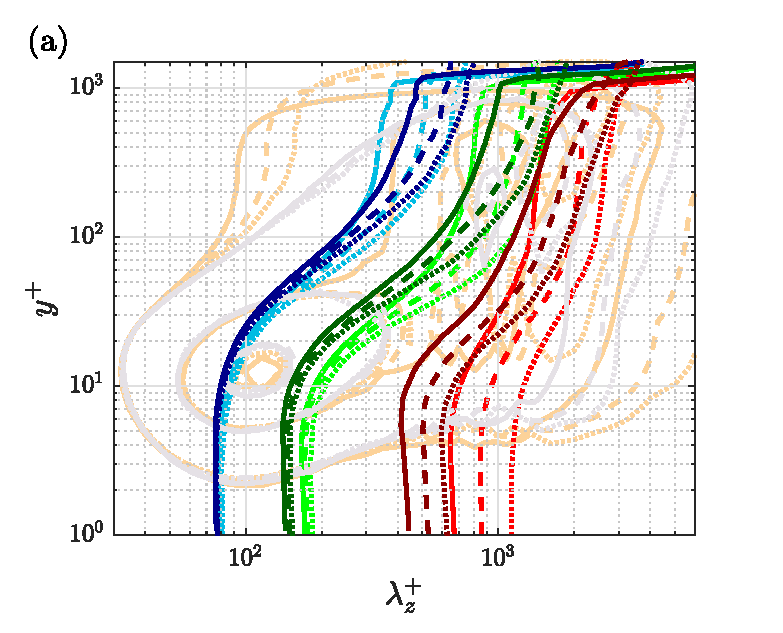
\includegraphics[width=0.45\textwidth]{imgs/spec/specMCE_uu_ltau_ltau.eps}
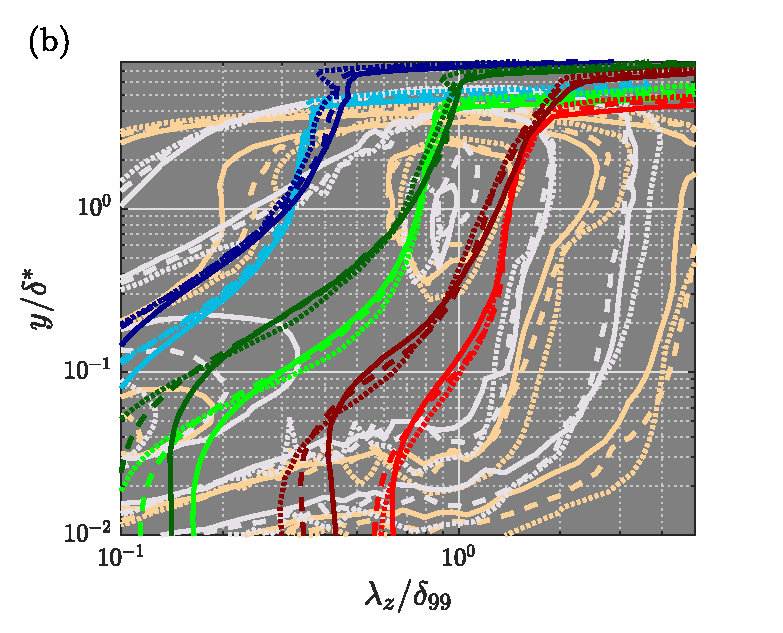
\includegraphics[width=0.45\textwidth]{imgs/spec/specMCE_uu_dstar_d99.eps}
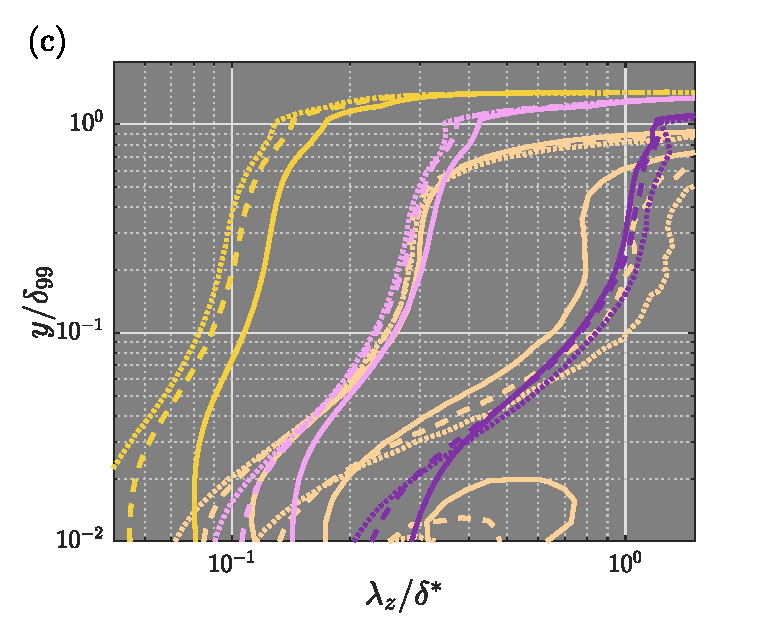
\includegraphics[width=0.45\textwidth]{imgs/spec/specMCE_uu_d99_dstar.eps}
\caption{ \label{fig:MCE_spec}
Contours of the premultiplied spectra $k_z\phi_{uu}$ in orange for b1.4 and light gray for the ZPG simulations.
The blue($20\%$), green($50\%$) and red($80\%$) lines are the MCE contours, where the light colors are used for the APG and the darker shades for the ZPG case.
Solid lines are used for $\Rey_{\tau}=1000$, dashed lines for $\Rey_{\tau}=1500$ and dotted lines $\Rey_{\tau}=2000$. Panel (a) shows the region that scales using inner scaling for both $y$ and $\lambda_z$; (b) scales the larger scales in the wake region by using two different length scales, $y\delta^*$ and $\lambda_z/\delta_{99}$. Panel (c) shows the scaling of the small-scale energy in the wake region characteristic of APGs, where $\lambda_z$ scales with $\delta^*$. The MCE contours are taken at $0.1\%$(yellow), $2.2\%$(pink) and  $15\%$(purple). 
}
\end{figure}







%===============================================================================
\chapter{Related Work}
%===============================================================================
%
%===============================================================================
\chapter{Conclusions and outlook}
%===============================================================================
%
%===============================================================================
\chapter{Test chapter, a very very very long title to test the table of contents}
%===============================================================================

This chapter is meant for testing the correct referencing of figures, equations
and tables.

% equations
%
\begin{equation}
	1 + 1 = 2
	\label{eq:test_eq1}
\end{equation}

\begin{align}
	2 + 2 = 4
	\label{eq:test_eq2}
\end{align}

\begin{equation}
	3 + 3 = 6
	\label{eq:test_eq3_intro}
\end{equation}

% tables
%
\begin{table}
	\centering
	\begin{tabular}{c}
		1
	\end{tabular}
	\caption{Test table 1}
	\label{tab:test_tab1}
\end{table}

\begin{table}
	\centering
	\begin{tabular}{c}
		2
	\end{tabular}
	\caption{Test table 2}
	\label{tab:test_tab2}
\end{table}

\begin{table}
	\centering
	\begin{tabular}{c}
		3
	\end{tabular}
	\caption{Test table 3}
	\label{tab:test_tab3_intro}
\end{table}

% figures
%
\begin{figure}[h!]
	\centering
	test figure 1
	\caption{Test figure 1}
	\label{fig:test_fig1}
\end{figure}

\begin{figure}[h!]
	\centering
	test figure 2
	\caption{Test figure 2}
	\label{fig:test_fig2}
\end{figure}

\begin{figure}[h!]
	\centering
	test figure 3
	\caption{Test figure 3}
	\label{fig:test_fig3_intro}
\end{figure}

% test references
%
\hrule
\begin{itemize}
	\item reference to equation 1: \eqref{eq:test_eq1}
	\item reference to equation 2: \eqref{eq:test_eq2}
	\item reference to equation 3: \eqref{eq:test_eq3_intro}
\end{itemize}
\hrule
\begin{itemize}
	\item reference to table 1: \eqref{tab:test_tab1}
	\item reference to table 2: \eqref{tab:test_tab2}
	\item reference to table 3: \eqref{tab:test_tab3_intro}
\end{itemize}
\hrule
\begin{itemize}
	\item reference to figure 1: \eqref{fig:test_fig1}
	\item reference to figure 2: \eqref{fig:test_fig2}
	\item reference to figure 3: \eqref{fig:test_fig3_intro}
\end{itemize}
\hrule

%===============================================================================
% Acknowledgments
%===============================================================================
%
\begin{acknowledgements}
% 	We would like to thank Gigi and SCIgen - An Automatic CS Paper Generator%
% 	\footnote{\url{https://pdos.csail.mit.edu/archive/scigen}}.
I would like to thank Ricardo Vinuesa and Philipp Schlatter first, without them I wouldn't have lived this wonderful adventure
which was to conduct my PhD studies in KTH. 
Qiang Li, a collaborator in my publications, but also a mentor, always encouraging me and ready to help. They have helped and guided me through my academic work and have always been there to share their knowledge an experience.
I also have to thank all those PhD's and professors that have made the life in the office so wonderful, in spite of the huge change that covid brought to our lifes.
Luca, Simon, Valerio and Vitor, with whom I lived my first "western" adventure. And the list goes on and on.
My family and friends in Spain that missed me so much, and my small "family" in Sweden for your moral support in good and dark times.
\end{acknowledgements}



%===============================================================================
% References
%===============================================================================
%
\bibliographystyle{jfm}
\bibliography{thesis}
%
% \IfFileExists{overview.bbl}{\graphicspath{{imgs/}}

%===============================================================================
\chapter{Introduction}
%===============================================================================
%
Throughout my academic career, I have enjoyed the step-by-step process of learning and I have discovered a passion for sharing my knowledge with friends, colleagues and some of my students.
In the same way the process of learning is unique, the process of teaching or communicating the knowledge should also be personal, trying to achieve the main goal of communication, transmitting correct information.
When we try to learn about a subject we can go to books, classes, different teachers, publications..., and sometimes we understand better from a book, other times from a video or a specific teacher or friend.
In this thesis, I will present some results on the physics of turbulent fluid mechanics where I have been involved, and I will try my best to communicate this knowledge to those interested in reading this work even if the reader is not very familiar with fluid dynamics.
Ideally, this transmission of knowledge should be concise, but I have experienced that certain complex knowledge sometimes requires different points of view or a simpler language. Personally, I like to communicate my knowledge as if it was a conversation instead of formal and impersonal writing.

Fluid mechanics or dynamics may sound as something complex for the non initiated, and it really is a complex science, but we already have intuitive and practical knowledge since we live and manipulate fluids every day so I will explain the basics.

A fluid is a substance that in contrast with a solid, it can easily deform and this property allows for the substance to adapt to containers or to move around other obstacles. An example is the air of the atmosphere, the liquid water in the sea, and even solids, like large accumulations of fine sand which subjected to vibrations can behave similar to liquid water.
Fluid mechanics is the science that studies everything related to the movement of fluids, like the forces involved or the properties of the fluid in its motion.

When a fluid moves around a solid (water around a rock), or the solid moves immersed in a fluid  (car moving through the air of the atmosphere) the fluid adapts to that relative motion by changing its properties, such as the velocity of its particles.
Where the fluid meets the solid, its particles have the same velocity as the solid because the forces in the interface fluid-solid (friction and pressure forces) are enough to deform the fluid.
The viscosity is the property of the fluid that opposes to the deformation. Inside the fluid, the viscosity is seeing as a force that reduces the velocity of the deformation or the velocity of the fluid particles.
In the example of the water in a river moving around a rock, far from the rock, the velocity of the water is that of the river, however the water in contact to the rock is not moving according to what we have explained earlier. The viscosity is responsible to adapt the velocity of the fluid from the velocity of the river to the velocity of the rock.
The change of velocity is actually done in a very small distance, and this region where the viscosity forces are adapting the fluid velocity is called boundary layer. 
The idea of boundary layer was introduced by Ludwig Prandtl in 1904 and it is the main topic of this thesis.

The boundary layers studied here are those pertaining to the momentum of the flow. The interest is in the effects of adverse pressure gradients in well-developed turbulent boundary layers. To avoid the influence of other effects we consider the simplest scenario.
The fluid is isotropic, incompressible and Newtonian, therefore the temperature does not change the density and the viscosity of the fluid.

The simplest solid boundary used is a flat plate without any heat or mass exchange (no suction or blowing). The adverse pressure gradient is then imposed as an outer boundary condition.
Comparisons can then be done with curved-boundary solids such as NACA profiles, where the pressure gradients are an aftereffect of the curvature of the profile. 
In these realistic configurations different mechanisms to control the flow are applied such as blowing or suction.

For these simple configurations we use a Cartesian system of coordinates where the space is denoted with $\vec{x}=x_i=(x,y,z)$, where we show the vectorial, dyadic and coordinate notations that will be used.
The boundary layers studied here are statistically 2D, $y$ is the wall-normal direction, $z$ is the homogeneous direction and $x$ is chosen as the streamwise direction. The time is denoted with $t$.
Although turbulence is a 3-dimensional (3D) phenomena, the flow analysed is statistically 2-dimensional, since there is an homogeneous direction. 

%-------------------------------------------------------------------------------
\section{Our Contribution}
%


\thesisstructure Add here a brief description of the structure of the thesis.

%===============================================================================
\chapter{Boundary layers, turbulence and pressure gradients}
%===============================================================================
%
% \begin{enumerate}
%     \item Physical phenomena
%     \begin{enumerate}
%         \item Elements involved (fluid and solid)
%         \item Properties of the elements that are meaningful for the problem
%         \item Observations or experimental knowledge $\rightarrow$ effects observed
%         \item New unseen problem $\rightarrow$ hypothesis of the effects to be observed
%     \end{enumerate}
    
%     \item Abstraction of the problem at hand and the physics
%     \begin{enumerate}
%         \item Equations for the physics studied (mechanics, thermal?, chemical?)
%         \item Mathematical model of the elements properties
%         \item Outer factors or conditions
%     \end{enumerate}
%     \item Analytical solution or numerical discretization.
%     \item Validation with experimental results
% \end{enumerate}

\graphicspath{{imgs/} {imgs/lam_turb} {imgs/spec}}

\section{Observations and empirical knowledge}

There are many examples of laminar and turbulent flows in nature that we are familiar with. In Fig.~\ref{fig:lam_turb} we show 3 examples, with water and flames. In the river image the water on the right side is laminar and on the left side it becomes turbulent. The calm flames of a candle rise initially in a laminar regime. On the bonfire example the flames are larger and show the different chaotic scale motions of a turbulent flow.

\begin{figure}[h!]
\centering
% \captionsetup{width=0.99 \textwidth}
\includegraphics[height=5cm ]{laminar_turbulent_1.jpg}
% \includegraphics[width=5cm ]{llama_laminar.jpg}
\includegraphics[height=5cm ]{velas.jpg}
\includegraphics[height=5cm ]{llama_turb1.jpg}
\caption{ \label{fig:lam_turb} Examples of ordered laminar flow and chaotic turbulent motions in water and fire.
   }
\end{figure}

Laminar and turbulent regimes presents its advantages and disadvantages. 
In aerodynamic applications we usually focus in minimizing the friction produced at the solid wall-boundary or maximizing the lift/drag coefficient. In that aspect, the laminar boundary layer produces less friction than a turbulent boundary layer because it alters less the flow.
Detachment of the flow is an undesirable effect produced by strong adverse-pressure gradients, in this aspect, the laminar flow structure is more sensible to detachment under APG conditions than a turbulent flow.

To study turbulent boundary layers (TBLs) and the effects of adverse pressure gradients (APG) we will compare APG TBLs with a TBL subjected to zero pressure gradient (ZPG) conditions. The case of favourable pressure gradients (FPGs) stabilizes and relaminarizes the boundary layer, and its effects are not critical such as those provoked by APGs, where the boundary layer can detach from the wall producing undesirable effects such as an increase in drag or even to loose the aerodynamic controls in airplanes.
In order to study this kind of wall-attached fluid problem, first we should analyze the elements involved, such as the fluid and the solid elements.

\section{Fluid properties}

When studying the mechanics of a solid we track the positions, velocities and accelerations, forces and torques along its movement in space and time. This is the Lagrangian approach to mechanics.
For a flow of particles or a fluid it is more interesting to observe the flow variables at specific locations and observe the temporal change of those variables at those locations. This is the Eulerian approach that will be used to study the mechanics of a fluid flow. 

The main variables are the fluid velocities, $\vec{u}(\vec{x},t)=u_i=(u,v,w)$, and the pressure $p(\vec{x},t)$.
To simplify the study of adverse pressure gradient turbulent boundary layers the fluid analysed is isotropic (its properties are the same in all directions) and Newtonian, this implies that the viscous forces are a linear function of the strain rate tensor $s_{ij}=\pdv{u_i}/{x_j}$. As an example, the friction at the wall is $\tau_w=\mu \pdv{u}/{y}$
where $\mu$ is a constant factor, the dynamic viscosity.
The density and viscosity of the fluid combines into the kinematic viscosity $\nu=\mu/\rho$ with units $[m^2/s]$ independent of the mass. 
Since we consider the density and viscosity as constant and not affected by changes in temperature, the temperature of the fluid is not relevant and the energy and momentum evolution are decoupled.

\section{Solid properties}
In general, the solid boundaries are curved specially in aerodynamic applications where the curvatures are used to create differences in pressures that lead to forces in the desired directions. The forces in the direction of the inflow are called drag and the forces in the perpendicular direction is called lift. For curved boundaries, different coordinate systems are used. The local system of coordinates that changes with the solid boundary is where the surface forces are calculated. The surface forces are then projected onto the global coordinates associated with the inflow to obtain the lift and drag.
For flat plates with zero angle of attack the global and local coordinates are the same.
The surface of the flat plate that we study is rigid, and smooth, and no exchange of heat or mass is produced between the fluid and the solid. In the interface fluid/solid the only interaction is due to pressure and viscous forces that adapts the fluid velocity to the solid surface velocity.
The flat plate will be considered to be static in the global system of coordinates.


\section{Boundary layers}

Boundary layers are regions inside a fluid flow where certain features or changes in the properties of the fluid are concentrated. Historically the first idea of boundary layer is set for the adaptation region of the fluid momentum from outer conditions to the dynamical conditions in a solid surface.
Other boundary layers are for example thermal boundary layers where the focus is on the change of thermal properties.

When we consider the flow around a solid object in an incompressible regime, the flow can detect the presence of the solid object and adapt its trajectory. The flow then surrounds the solid starting from the leading edge and close to the solid surface the boundary layer is the region where the velocity of the flow adapts from the solid surface velocity to the outer flow velocity. The boundary layer thickness have to be defined according to the main idea of a region of the fluid close to the solid wall that encloses the major viscous effects created due to the fluid/surface interaction. An obvious effect of the presence of a wall is that the streamwise velocity has to adapt from the velocity of the solid boundary to the exterior velocity, commonly called velocity at the infinity $U_{\infty}$. 
In general, for a certain position of the wall, the velocity is measured in the wall-normal direction, obtaining a profile of streamwise velocities $u(y,t)$. Then $U_{\infty}=u(y\rightarrow \infty)$ is the unperturbed velocity and can change from one streamwise position to another.
In the case of zero-pressure gradient boundary layers, $U_{\infty}$ is taken as constant, since in a steady flow in the absence of viscous forces, $\pdv{u}/{x}$ should be zero. 

Since an obvious indicator of the boundary layer is the adaptation of the streamwise velocity, the boundary layer can be defined using this property and the $99\%$ thickness $\delta_{99}$ is defined as the wall-normal position where $u(y=\delta_{99}) = U_{\infty}$.
In Fig.~\ref{fig:lam_turb_profiles} we show an example on how the mean streamwise velocity $U(y)$ adapts from the velocity at the wall $u(y=0)=0$, to the outer velocity $U_{\infty}$, which has been scaled to be equal to 1, on a laminar and a TBL ZPG profiles.

\begin{figure}[h!]
\centering
% \captionsetup{width=0.99 \textwidth}
\includegraphics[width=0.5\textwidth]{ZPG_lam_turb.jpg}
\caption{ \label{fig:lam_turb_profiles} Mean streamwise velocity profile of a laminar (blue) and a turbulent ZPG (red) boundary layers.
   }
\end{figure}

In the case of curved boundaries, the curvature induces a pressure-gradient since the incoming flow has to adapt to the curvature of the wall. In a flat plate, a pressure-gradient can be produced by controlling the exterior flow, usually the streamwise gradient of the streamwise velocity $\pdv{U_{\infty}}/{x}$


\subsection{Turbulent boundary layers}
The characteristics of a boundary layer changes radically depending on the laminar/turbulent regime.
In a laminar boundary layer, any perturbation produces shear stresses and therefore, viscous forces, which are transported by the momentum of the flow and eventually dissipated by the viscous dissipation. 
High energetic perturbations, flow configurations or certain viscosity/momentum forces ratios are unstable, implying a change of regime, usually from the laminar regime to turbulence. 
The ratio between momentum and viscous forces is called Reynolds number $\Rey=U_{sc} L_{sc} / \nu$ and depending on the velocity scale $U_{sc}$ and the $L_{sc}$ chosen we would be analyzing different phenomena. The Reynolds number where a fluid configuration changes regime is called critical Reynolds number $\Rey_c$.
Other Reynolds number examples: if $U_{sc}=U_{\infty}$ and $L_{sc}=c$ where $c$ is the chord of a NACA profile, then we are setting the global configuration of the problem. If we want to analyze a local phenomena such as the different size of the fluid scales close to the wall compared to the largest ones inside the TBL, then we can use the Reynolds number based on the friction velocity $\Rey_{\tau}=u_{\tau}\delta_{99}/\nu$, where  $u_{\tau}(x)=\sqrt{(\tau_w / \rho)}$.

In the turbulent regime, the momentum and energy of the flow initiates a cascading effect breaking the initial ordered motions into chaotic submotions. 
Eddies are generated that extract energy from the mean flow and are divided into smaller eddies. Then a transport of energy between large and small eddies is produced. Eddies are regions with strong shear stresses, therefore the viscous forces are stronger and produce a dissipation of the kinetic energy.
The boundary layers studied here are momentum boundary layers that confine the turbulent perturbations and mayor viscous effects produced because of the presence of a solid boundary.

In a turbulent boundary layer, the thickness of the boundary layer should capture both the effects of the viscous forces as well as the turbulent fluctuations produced because of the presence of a solid boundary, leading to different definitions for the boundary layer thickness.

For laminar BLs and ZPG TBLs, the previous $\delta_{99}$ thickness, where the mean velocity of the flow is $99\%$ of the exterior velocity, is valid and is based only on the adaptation of the mean streamwise velocity to that of the outer flow.

For other TBLs with pressure gradients, the outer velocity can have gradients in the streamwise and wall-normal directions even without the presence of turbulence. In this case we can use an approach based on the level of turbulence such as the one used in \cite{diagnostic_Vinuesa} where the boundary layer thickness is such that it captures the turbulence up to certain turbulent level.
This approach is useful for the dataset that we use, since the turbulent levels outside of the TBL are minimal, both in the simulations \citep{E-AmorZPG, bobke2017, Pozuelo_JFM_22}, as in the experimental databases \citep{Sanmiguel_PRF}.
If the outer flow turbulent level is high, the method in \cite{diagnostic_Vinuesa} is not applicable. 
Other methods have been proposed in the literature and a review was given in \cite{d99_determination_2020}.

Turbulence presents a wide range of motions, the way we have been able to study and characterize turbulence is through decomposition of those characteristics. 
The first approach is an statistical characterization where we can divide the fluid variables into a mean or average value and a perturbation, this is known as the Reynolds decomposition \citep{Rey_decomp}.
The fluctuating character of the flow is shown for a flat plate APG TBL in Fig.~\ref{fig:lam_turb_development} where we show contour levels in snapshots of the instantaneous streamwise velocity. The contours in Fig.~\ref{fig:lam_turb_development}(a) are smooth and show a well-defined laminar behaviour with small perturbations introduced to trigger turbulence. In Fig.~\ref{fig:lam_turb_development}(b) the turbulence is totally developed It can be seen how at different streamwise positions $x/\delta^*_0$ the outer velocity or "edge velocity" $U_e$ decreases along $x$ to obtain an APG. The edge velocity is the velocity of the TBL at $y=\delta_{99}$ and depends on the method used to determine the boundary layer thickness.

\begin{figure}[h!]
\centering
% \captionsetup{width=0.99 \textwidth}
\includegraphics[width=0.49\textwidth ]{APG_laminar.jpg}
\includegraphics[width=0.49\textwidth]{APG_turb.jpg}
\caption{ \label{fig:lam_turb_development} Snapshot of the streamwise velocity $u(\vec(x), t)$ in a laminar (a) and a turbulent APG (b), boundary layers.
   }
\end{figure}



\section{Mathemathical analysis}

For an incompressible flow the conservation of mass in a control volume becomes the differential continuity equation (Eq.~\ref{eq:continuity_cap2}),

% Continuity
\begin{equation}
\label{eq:continuity_cap2}
% \overrightarrow{u}
    \nabla \cdot \vec{u} = \partial_i u_i = 
    \frac{\partial u}{\partial x} + \frac{\partial v}{\partial y} + \frac{\partial w}{\partial z} = 0,
\end{equation}
which is shown as the divergence of the velocity vector, the diadic and components notations.

To describe the time evolution of the fluid variables, the partial differential equations in Eq.~\ref{eq:NS_cap2} are the Navier--Stokes (NS) equations that describes the evolution of the momentum of the fluid as a function of the pressure gradient and viscous forces acting on it. The system of equations composed by Eqs.~\ref{eq:continuity_cap2} and \ref{eq:NS_cap2} are able to give both laminar and turbulent flow regimes, depending on the configuration of the problem.

% NS Total velocities
\begin{equation}
    \label{eq:NS_cap2}
    \frac {\partial u_i} {\partial t}  + u_j \frac {\partial u_i} {\partial x_j} =
    \frac {-1} {\rho} \frac {\partial p} {\partial x_i} +  \nu \frac {\partial^2 u_i} {\partial x_j^2}.
\end{equation}

By giving the correct scenario which is the boundary conditions (BCs) composed by an inflow, outflow, outer flow and wall-boundary conditions, together with an initial state of the system, we can expect either laminar flow or the change into a turbulent flow.



Once turbulence is fully-developed, the statistical approach to turbulence is based on the Reynolds decomposition \citep{Rey_decomp}, given in Eq.~\ref{eq:Rey_decomp}. This decomposition is based on a constant or averaged component and a fluctuating component in a way that once they are inputted into Eqs.~\ref{eq:continuity_cap2} and \ref{eq:NS_cap2} some of the partial differentials are simplified. An example is to use a constant base flow (such as the laminar state) plus a fluctuating flow field, this is the case used to study transition and stability of BLs. 
For our case, the mean flow $U_i$ is an average in time and the homogeneous directions. The average in a dimension $d$ is marked as $\langle . \rangle_d$, and the average in time and all the homogeneous dimensions is marked with $\overline{(.)}$. The mean velocity is $U_i = \overline{u_i} =\langle \langle u_i \rangle_z \rangle_t$ and as a result of Eq.~\ref{eq:Rey_decomp}, $\overline{u_i\myprime}=0$. Note that $\langle u_i\myprime \rangle_z (t) \neq 0$ and $\langle u_i\myprime \rangle_t(z) \neq 0$. 

Introducing the flow decomposition (Eq.~\ref{eq:Rey_decomp}) into the continuity and NS equations (Eqs.~\ref{eq:continuity_cap2} $\&$ \ref{eq:NS_cap2}), and using the total average in time and $z$, we see that the continuity equation is fulfilled for both the mean and the fluctuating component separately (Eq.~.\ref{eq:cont_decomp}). And in the NS equation we obtain the Reynolds Averaged Navier--Stokes equation (RANS) in Eq.~\ref{eq:RANS_cap2} and the equation for the time evolution of the perturbations Eq.~\ref{eq:pertub_cap2} as a result of substracting the RANS equations from the general NS equations.

% R Decomposition
\begin{equation}
    \label{eq:Rey_decomp}
    u_i = U_i + u_i\myprime.
\end{equation}

\begin{equation}
    \label{eq:cont_decomp}
    \partial_i \overline{u_i} = \partial_i \overline{U_i} = 0 ~~~~
    \partial_i \overline{U_i} + \partial_i \overline{u_i\myprime} = 0.  
\end{equation}

% RANS
\begin{equation}
    \label{eq:RANS_cap2}
    U_k\pdv{U_i}{x_k} + \pdv{\overline{u_i\myprime u_k\myprime}}{x_k} = \frac {-1} {\rho} \frac {\partial P}{\partial x_i} + \nu  \frac {\partial^2 U_k} {\partial x_k^2}.
\end{equation}

% Perturbations
\begin{equation}
    \label{eq:pertub_cap2}
    {\pdv{u_i\myprime}{t} + 
    U_k\pdv{u_i\myprime}{x_k} + u_k\myprime\pdv{u_i}{x_k} - \pdv{\overline{u_i\myprime u_k\myprime}}{x_k}  =
    \frac {-1} {\rho} \pdv{p\myprime}{x_i} + \nu  \frac {\partial^2 u_k\myprime} {\partial x_k^2}    }.
\end{equation}

Note that the RANS equation are similar to the NS equation, except that for the time derivative which is zero and an aditional term $\pdv{\overline{u_i\myprime u_k\myprime}}/{x_k}$ which can be included within the divergence of the viscous forces term, for that reason the terms $\rho \overline{u_i\myprime u_k\myprime}$ are called Reynolds-stresses. In the following, since the density is considered as constant, we will refer as Reynolds-stress (RS) to the terms in the tensor $\overline{u_i\myprime u_k\myprime}$, wich are also known as the variance or covariance of the total velocities $u_i$, $u_k$.
From the RANS equations it is interesting to see the mean velocities and the RS terms since they are an indicative of the level of turbulence and how it is affected by the pressure gradients and viscous forces on the right hand side (RHS) of the equation.

The equation for the perturbation velocities is useful since we can multiply by another perturbation velocity such as $u_{j}\myprime \cdot \left( \pdv{u_{i}\myprime}{t} + ... \right) $ or obtain the two-point correlation $\mathcal{R}_{u_i\myprime u_j\myprime}$ through the correlation denoted with the symbol $(\cdot \star \cdot)$ as in $ u_{i}\myprime \star \left( \pdv{u_{j}\myprime}{t} + ... \right)$. The former gives the Reynolds-stress transport equations (Eq.~\ref{eq:RS_transport_cap2}) where the turbulent kinetic energy budgets are a special case. The latter is used as in \cite{lee_moser_2019}, to obtain the power spectral density of each term of the Reynolds-stress transport equations.

Denoting Eq.~\ref{eq:NS_cap2} as $\mathrm{TOT}_i$, Eq.~\ref{eq:RANS_cap2} as $\mathrm{RANS}_i$ and Eq.~\ref{eq:RS_transport_cap2} as $\mathrm{PERT}_i$, the evolution equation for the total kinetic energy of the flow can be obtained through the multiplication,
% $\mathrm{KE} = (1/2) \overline{u_i \cdot \mathrm{TOT}_i}$, 
\begin{equation}
    \mathrm{KE} = (1/2) \overline{u_i \cdot \mathrm{TOT}_i}, 
\end{equation}
while the mean kinetic energy equation can be obtained with 
% $\mathrm{MKE} = (1/2) U_i \cdot \mathrm{RANS}_i$,
\begin{equation}
    \mathrm{MKE} = (1/2) U_i \cdot \mathrm{RANS}_i,
\end{equation}
and the turbulent kinetic energy equation with 
% $\mathrm{TKE} = (1/2) \overline{u_i\myprime \cdot \mathrm{PERT}_i} = KE - MKE$.
\begin{equation}
    \mathrm{TKE} = (1/2) \overline{u_i\myprime \cdot \mathrm{PERT}_i} = KE - MKE.
\end{equation}
In a similar way the Reynolds-stress transport ($RST_{ij}$) equation Eq.~\ref{eq:RS_transport_cap2} can be obtained by doing 
% $\mathrm{RS}_{ij} = \overline{u_i\myprime \cdot \mathrm{PERT_j} + u_j\myprime \cdot \mathrm{PERT_i}} $
\begin{multline}
    \mathrm{RST}_{ij} = \overline{u_i\myprime \cdot \mathrm{PERT_j} + u_j\myprime \cdot \mathrm{PERT_i}} = \\
    = \overline{u_i \cdot \mathrm{TOT_j} + u_j \cdot \mathrm{TOT_i}} - (U_i \cdot \mathrm{RANS}_j + U_j \cdot \mathrm{RANS}_i ) .
\end{multline}
% $\mathrm{RS}_{ij} = \overline{u_i \cdot \mathrm{TOT_j} + u_j \cdot \mathrm{TOT_i}} - (U_i \cdot \mathrm{RANS}_j + U_j \cdot \mathrm{RANS}_i )$.
% \begin{equation}
%     \mathrm{RS}_{ij} = \overline{u_i \cdot \mathrm{TOT_j} + u_j \cdot \mathrm{TOT_i}} - (U_i \cdot \mathrm{RANS}_j + U_j \cdot \mathrm{RANS}_i ) .
% \end{equation}

% RS transport equation
\begin{multline}
    \label{eq:RS_transport_cap2}
    \pdv{\overline{u_i\myprime u_j\myprime}}{t} + 
    U_k\pdv{\overline{u_i\myprime u_j\myprime}}{x_k} + 
    \left(
    \overline{u_i\myprime u_k\myprime}\pdv{U_j}{x_k} + \overline{u_j\myprime u_k\myprime}\pdv{U_i}{x_k}
    \right) +
    \left(
    \overline{u_i\myprime \pdv{u_j\myprime}{x_k} u_k\myprime} + \overline{\pdv{u_i\myprime}{x_k} u_j\myprime u_k\myprime}
    \right)
    = \\ 
    - \left( \overline{
    u_j\myprime \pdv{p\myprime}{x_i} + u_i\myprime \pdv{p\myprime}{x_j}
    } \right) 
    + \nu \frac{\partial^2 \overline{u_i\myprime u_j\myprime}}{\partial x_k^2} 
    - 2\nu \overline{\pdv{u_i\myprime}{x_k} \pdv{u_j\myprime}{x_k}}
\end{multline}

The third term in Eq.~\ref{eq:RS_transport_cap2} is specially interesting, after some manipulation, that term appears in the transport of $U_iU_j$ and the transport of $\overline{u_i\myprime u_j\myprime}$ with different signs. Usually is written on the right hand side of the equation and is called ``Production" since it substract energy from the mean flow and adds into the perturbations.
The other terms are presented in Appendix B from \textbf{Paper 1}.



%===============================================================================
\chapter{Numerical experiments on flat plate turbulent boundary layers}
%===============================================================================
%

\section{Turbulent Boundary layers under adverse pressure gradients}

A wall-bounded flow can see pressure gradients as a result of the curvature of the wall, but also as a result of a change in the direction/velocity of the outer flow $(U_{e}, V_{e}, W_{e})$. Turbulence is already a complex problem in a ZPG case with the only parameter being the Reynolds number (momentum/viscous forces), if another parameter such as pressure gradients is added, the complexity of the problem increases and it becomes difficult to distinguish what phenomena is caused by the $\Rey$ effects or by the PG history of the flow.
In order to properly study APG TBLs, first we should try to define a canonical simple case, that is a well-defined APG along the streamwise development of the TBL, this is what we refere as the PG history of the flow.
To address this problem, different pressure-gradient parameters have been defined in literature, such as the Rotta-Clauser PG parameter $\beta$, or a general $\Lambda_{inc}$ which in \cite{Gibis2019} is studied with different length and velocity scales.
In our simulations of moderate APGs we have used $\beta$ defined as
\begin{equation}
    \beta(x) = \frac{\delta^*}{\tau_w} \pdv{P}{x},
\end{equation}
where $\pdv{P}/{x}$ is the averaged pressure-gradient, $\tau_w$ is the mean shear stress at the wall, and $\delta^*$ is the displacement thickness, which for an incompressible flow is defined as
\begin{equation}
    U_e \delta^* = \int_{0}^{\delta_{99}} (U_e - U) dy
\end{equation}

% IDEA behind beta
The idea behind the $\beta$ parameter is to stablish an integral equilibrium of forces across the TBL, in this way, every section of the TBL is subjected to the same dimensionless state of forces.
To clear this idea, Fig.~\ref{fig:scheme_beta} shows a scheme of a section of the BL, where the main forces are due to the streamwise pressure-gradient and the stress at the wall.

\begin{figure}
    \centering
    \includegraphics[width=0.90\textwidth]{imgs/schemes/scheme_beta.jpg}
    \caption{Stresses around a section of a BL.}
    \label{fig:scheme_beta}
\end{figure}

Integrating the streamwise momentum equation over the wall-normal direction, under several assumptions, it is possible to obtain an equation which relates the integral parameters $\delta^*$, $\theta$ and $\beta$, therefore, from an integral approach, the thickness $\delta \myprime$ is chosen equal to $\delta^*$. 



\section{Statistics}
In \textbf{Paper 1} we explore the statistical quantities of TBLs under APGs. The novelty respect to the available literature was in the high fidelity database used for the ZPG and APG TBLs. Both simulations show the development of the TBL from low Reynolds numbers such as those of previous numerical databases, and reach large Reynolds numbers such as those obtained in experiments. This characteristic works as a bridge to validate previous simulations as well as the current simulations, since they have been compared successfully with experimental data.
A benefit of numerical experiments is that the amount of quantities measured are larger than in experimental databases. This allows to have better measurements close to the wall and obtain decomposition such as spanwise spectra.

\begin{table}
  \begin{center}
  \fontsize{8.0pt}{10.25pt}\selectfont
  \addtolength{\tabcolsep}{-2pt}
\def~{\hphantom{0}}
    \begin{tabular}{ l r  r  r }
    Case  & Colour & Reference \\[3pt]
    \hline
    b1             & \redline     & Bobke (\citeyear{bobke2017}) \\
    b2             & \greenline   & Bobke (\citeyear{bobke2017}) \\
    m16            & \blueline    & Bobke (\citeyear{Bobke_2016}) \\

    ZPG            & \blackline   & Eitel-Amor (\citeyear{E-AmorZPG}) \\
    b1.4           & \orangeline  & Pozuelo (\citeyear{Pozuelo_JFM_22}) \\
    exp            & \redcircle   & SanMiguel (\citeyear{MTL_expSANMIGUEL}) \\
    \hline
    \end{tabular}
  \caption{ Line styles and colors used for the simulations and experiments used in the thesis.}
  \label{tab:param_cap2}
  \end{center}
\end{table}

% \begin{table}
%   \begin{center}
%   \fontsize{8.0pt}{10.25pt}\selectfont
%   \addtolength{\tabcolsep}{-2pt}
% \def~{\hphantom{0}}
%     \begin{tabular}{ l r  r  r  r  r  r  r  r  r  r  r r}
%     Case  & $L_x/\delta_0^*$ & $L_y/\delta_0^*$ & $L_z/\delta_0^*$ & $m_{x}$ & $m_{y}$ & $m_{z}$ & $\Delta x^{+}$ & $\Delta y_{\rm max}^{+}$ & $\Delta z^{+}$ & Colour & Reference \\[3pt]
    
%     b1             &    3000   &   140   &    250  &    3072 &     301 &     576 &   21.8    & 8.4 &   9.7  & \redline     & Bobke (\citeyear{bobke2017}) \\
%     b2             &    3000   &   180   &    320  &    3072 &     361 &     768 &   21.6    & 7.9 &   9.2  & \greenline   & Bobke (\citeyear{bobke2017}) \\
%     m16            &    3000   &   180   &    220  &    3072 &     361 &     576 &   21.2    & 7.7 &   8.3  & \blueline    & Bobke (\citeyear{Bobke_2016}) \\

%     ZPG            &   13500   &   400   &    540  &   13824 &     513 &    1152 &   22.6    & 19.6 &  10.9  & \blackline  & Eitel-Amor (\citeyear{E-AmorZPG}) \\
%     b1.4           &   13500   &   800   &   1080  &   13824 &     301 &    1920 &   21.7    & 30.1 &  12.5  & \orangeline & Present study \\

%     \end{tabular}
%   \caption{
% %   Parameters of the simulations used in this paper. The inlet displacement thickness $\delta_0^*$ corresponds to the displacement thickness of a laminar flow for a Reynolds number $Re_{\delta_0^*}=450$. The box size is $(L_x/\delta_0^*, L_y/\delta_0^* , L_z/\delta_0^*)$  and $(m_x, m_y, m_z)$ are the number of collocation points including the $3/2$ factor for de-aliasing in the Fourier directions ($x$ and $z$). The spatial resolution in viscous units $(^+)$ of the streamwise and spanwise directions $\Delta x^{+}, \Delta z^{+}$, has been calculated using $(m_x, m_z)$ at the position $x/\delta_0^*=250$, which corresponds to a friction Reynolds number $Re_{\tau}\approx 210$ for all the simulations. The maximum viscous distance between grid points in the wall-normal direction inside the boundary layer is observed close to the boundary-layer edge and for the highest Reynolds number of each simulation. 
%   }
%   \label{tab:param_cap2}
%   \end{center}
% \end{table}


In Fig.~\ref{fig:U_uu_cap2}(a) we show the inner scaled $U$ and $\sqrt{\overline{u\myprime u\myprime}}$ for a $\Rey_{\tau}=500$, where the low Reynolds number simulations are already fully developed, while the experimental database does not have measurements. A higher $\Rey_{\tau}=2000$ is required by the experiments to have a fully developed near-equilibrium APG, and the LES ZPG and the new b1.4 simulation are able to achieve those Reynolds numbers.
The experimental data \citep{MTL_expSANMIGUEL} and b1.4 are in a similar range of $\beta$ and their statistics show a good agreement in the streamwise components.
The effects of the APG in $U$ show a lower $U^+$ for larger $\beta$ in the logarithmic region, and a larger effect in the wake region. At higher Reynolds numbers, the logarithmic region enlarges and the near-equilibrium APG and the ZPG profiles get closer.
In the turbulent perturbations, the near-wall or inner peak of $\sqrt{\overline{u\myprime u\myprime}}^+_{IP}$ grows in value with both the Reynolds number and the APG effects and its wall-normal position $y_{IP}^+$ seems to slightly increase with both APG and $\Rey$ effects. In \cite{Pozuelo_JFM_22} this trend is shown, where a filter was used to avoid saw-tooth jumps due to the wall-normal resolution close to the wall.
Larger Reynolds numbers allows for larger scales to live in the logarithmic/wake region and for a separation of the scales to be seen. This is first seen as lower decay in $\sqrt{\overline{u\myprime u\myprime}}$ in the ZPG in the logarithmic/wake region and a development of an outer peak for APG profiles. Larger $\beta$ increase the value of the outer peak of $\sqrt{\overline{u\myprime u\myprime}}$. The trends for the outer peak value and wall-normal position of the RS,  $\overline{u\myprime u\myprime}_{OP}$ and $y_{OP}$ where analysed in \cite{Pozuelo_JFM_22}. 


\begin{figure}
    \centering
    \includegraphics[width=0.49\textwidth]{imgs/stats/U_uu_a.eps}
    \includegraphics[width=0.49\textwidth]{imgs/stats/U_uu_b.eps}
    \caption{Mean streamwise $U$ (solid lines) and streamwise root mean square $u_{rms}$ or strandard deviation of the streamwise velocity (dashed lines). Wall-normal profiles taken at: (a) $\Rey_{\tau}=500$, (b) $\Rey_{\tau}=2100$. }
    \label{fig:U_uu_cap2}
\end{figure}

\subsection{Friction at the wall, on the friction coefficient $c_f$}

The drag in aerodynamic structures has an important contribution from the friction at the wall, also known as skin friction which is the mean shear stress produced at the wall $\tau_w$, due to the viscous forces.
Instead of $\tau_w$, it is common to look at the friction factor $c_f$ which is a ratio between the friction stresses and the free flow,
\begin{equation}
    c_f = \frac{\rho \tau_w}{1/2 \rho U_e^2} = \frac{2 u_{\tau}^2}{U_e^2} = 2\left( \frac{u_{\tau}}{U_e} \right)^2
\end{equation}
but it can also be seen as an indicator of the friction-velocity with respect to the free-flow velocity.

\begin{figure}
    \centering
    \includegraphics[width=0.85\textwidth]{imgs/stats/cf_Retau.eps}
    \caption{Evolution of the mean friction coefficient $c_f = \pdv{2\overline{\tau_w}}/{U_e^2}$ for ZPG and APG simulations (solid lines) and experiments by \cite{MTL_expSANMIGUEL} (red circles).}
    \label{fig:cap3_evol_cf}
\end{figure}

In Fig.~\ref{fig:cap3_evol_cf} we show the mean friction factor development along the turbulent boundary layers for ZPG and APG simulations and an experimental APG.
It can be seen how for attached flows and near-equilibrium TBLs the trend is positive, decays with the Reynolds number and the value is lower the stronger the APG intensity.
The simulations show an increase for the larger $\Rey_{\tau}$ where the fringe region starts to affect the flow, and this region is not included in the region of interest (ROI) of our database.

The effects of APG on the coefficient $c_f$ are studied through the Renard--Deck (RD) \citep{Renard2016} identity in \textbf{Paper 3} and the Fukagata, Iwamoto \& Kasagi identity (FIK)  \citep{Fukagata2002} in \textbf{Paper 4}.

The FIK decomposition of $c_f$ is adapted to include a join contribution of the pressure gradient and the streamwise convection, looking for a dynamic pressure perspective, instead of treating this antagonizing contributions as a separate entity.

A different approach onto the $c_f$ is that of the RD decomposition, taken from a perspective based on the mean streamwise kinetic energy budget. 
The main contributions to the total $c_f$ are divided in three main terms representing the viscous dissipation, the turbulent kinetic energy production and the spatial growth.
The contribution from the viscous diffusion is mainly located in the inner/near-wall region of the TBL and the influence diminish for stronger APGs, since the influence of the larger scales located in the outer region of the TBL are more energized and its effects on $c_f$ are larger.
The TKE Production close to the wall have a near-wall peak that influences $c_f$, but the influence of APGs produce a strong outer-peak in the outer region.
The spatial growth contribution is further decomposed into three subterms, the main ones are due to the mean convection $\Vec{U}\cdot \nabla\Vec{U}$ (which has a positive contribution across the TBL) and a direct contribution of the pressure-gradient (which has a negative contribution on $c_f$). These terms are more relevant the stronger the APG is and decrease with $\Rey$, and their influence is mostly located in the outer/wake region of the TBL.


\section{Spectral decomposition}
To have a better understanding on the perturbations we can use some mathematical tools such as the decomposition of the spatial-temporal signal using correlations, orthogonal modes, coherent structures, etc.
The use of orthogonal modes allows to decompose the energy of the perturbations into each mode in an unique way, so the sum of the energy contained in all the modes is equivalent to the total energy of the perturbations. 

In signal analysis an orthogonal decomposition which is commonly used is the Fourier decomposition which enables to look for phenomena that repeats with a certain time or spatial frequency. The energy or power associated with each mode is called energy spectra (if the signal is finite such as pulses) or power spectra (if the signal is such as sinusoidal waves, whose domain and energy is not finite, however its power is). Remember that the power is the ratio of the energy over time, where the time goes to infinity (in the case of using temporal series).
Since we are dealing with signals which are periodic in the homogeneous dimension $z$ and are not limited in time, we will use the terminology of power spectra (PS) instead of energy spectra. 
The modes in $z$ have a wavenumber $k_z$ and a wavelength $\lambda_z=2\pi/L_z$ where $L_z$ is the spanwise period of the domain. The same analysis can be applied in time, where we will use $k_t$ and $\lambda_t$.
For a signal $x(t)$, with $X(k_t)$ being its Fourier transform, the power of each mode is $|X(k_z)|^2$, the squared amplitude of the mode. For a perturbation velocity, the power can be calculated as,
\begin{equation}
    PS_{u_i\myprime u_j\myprime}(k_z) = \mathcal{F}(u_i \myprime)  \mathcal{F}^*(u_j \myprime),
    \label{eq:power_sp}
\end{equation}
where $\mathcal{F}()$ is the Fourier transform and $\mathcal{F}^*()$ represents the complex conjugate and the definition has been expanded to include the power spectra of the quantity $\langle u_i\myprime u_j\myprime \rangle_{z}$, also known as cospectra.
Using the properties of the Fourier transform, the multiplication in Fourier space represented in Eq.~\ref{eq:power_sp} represents the Fourier transform of the two-point correlation function $\mathcal{R}_{u_i\myprime, u_j\myprime}(\delta z)=u_i\myprime \star u_j\myprime$, where $\delta z$ is the lag or distance between the two points where we look for the correlation of their velocity perturbations. According to the Wiener--Khinchin theorem, we can calculate the PS through as the Fourier transform of $\mathcal{R}_{u_i\myprime, u_j\myprime}$ or from the power spectra throught the inverse Fourier transform $\mathcal{F}^{-1}()$ we can obtain the two-point correlation function.

Note that for velocity perturbations, since Fourier modes are orthogonal, the sum of the PS for all the modes is equal to the averaged Reynolds stress,
\begin{equation}
    \langle u_i\myprime u_j\myprime \rangle_{z} = \sum_{k_z} PS_{u_i\myprime u_j\myprime}(k_z)
\end{equation}

This step can be performed for each time step and averaged over time to obtain $\langle\langle u_i\myprime u_j\myprime \rangle_{z}\rangle_{t} = \overline{u_i\myprime u_j\myprime}$ or it can also be the result of a 2D spectral decomposition in both time and $z$, where the sum extends to all the spatial and temporal modes.

The PS is useful for discrete systems, and it is the first step when we calculate numerically the spectra of a the Reynolds-stresses. It is also interesting to see how the power spectra is distributed along the wavenumbers or the wavelengths, obtaining a power spectral density (PSD).
The average in time of the PSD in wavenumbers is $\phi_{u_i\myprime u_j\myprime}=\langle PS \rangle_t/\mathrm{d} k_z$ while the average in time PSD in wavelengths is $\psi_{u_i\myprime u_j\myprime}= \langle PS \rangle_t/\mathrm{d} \lambda_z$. Both densities can be linked using $\mathrm{d}(\lambda_z) = \mathrm{d}(2\pi/k_z) = -2\pi\mathrm{d}k_z/k_z^2$:

\begin{equation}
    \psi_{u_i\myprime u_j\myprime} = 
    \frac{ \langle PS_{u_i\myprime u_j\myprime} \rangle_t}{\mathrm{d} \lambda_z} =
    -\frac{ \langle PS_{u_i\myprime u_j\myprime} \rangle_t}{\mathrm{d} k_z} \frac{k_z^2}{2\pi},
\end{equation}
where the minus sign is taking care by inverting the limits of integration to obtain the total RS (small to large wavenumbers is equivalent to integrate from large to small wavelengths).

\begin{equation}
\label{eq:sum_ps}
    \overline{u_i\myprime u_j\myprime} = 
    \int_{k_z=k_0}^{k_z=k_{N}}   \phi_{u_i\myprime u_j\myprime}  ~ \mathrm{d} k_z =
    \int^{\lambda_z = 2\pi/k_0}_{\lambda_z = 2\pi/k_{N}}  \psi_{u_i\myprime u_j\myprime}  ~ \mathrm{d} \lambda_z
\end{equation}

In Fig.~\ref{fig:PS_PSD} we show for a ZPG TBL, different representations of the PSD of $\overline{u\myprime u\myprime}$ where the image with the black contours represent a streamwise profile at $\Rey_{\tau}=2000$ while the red contours are taken at a position where $\Rey_{\tau}=500$.

\begin{figure}[h!]
\centering
% \captionsetup{width=0.99 \textwidth}
\includegraphics[width=0.32\textwidth ]{imgs/spec/ZPG_Ret_500_2000_PSdkz_kz_ltau_y_ltau.jpg}
\includegraphics[width=0.32\textwidth]{imgs/spec/ZPG_Ret_500_2000_PSdlambdaz_lambdaz_ltau_y_ltau.jpg}
\includegraphics[width=0.32\textwidth]{imgs/spec/ZPG_Ret_500_2000_kPSdkz_lambdaz_ltau_y_ltau.jpg}
\caption{ \label{fig:PS_PSD} Spanwise spectra of the streamwise Reynolds stress $\overline{uu}(y)$. (a) Power spectral density $\phi_{u\myprime u\myprime}(y,k_z)$; (b) Power spectral density $\psi_{u\myprime u\myprime}(y,\lambda_z)$; (c) premultiplied power spectral density $k_z\phi_{u\myprime u\myprime}$. Wavenumbers, wavelengths, wall-normal position and power spectra scaled in viscous units.}
\end{figure}
% contours: Retau 2000: [40 80  120 400 600]; [0.001 0.005 0.02 0.035 0.04] ;  [ 0.5 2 3.5]; 
% contours: Retau  500: [40 80  120        ]; [0.001 0.005 0.02 0.035 0.04] ;  [ 0.5 2 3.5]; 

The PS and the PSD in the wavenumbers $\phi_{u\myprime u\myprime}(y,k_z)$ present the same features as in Fig.~\ref{fig:PS_PSD}(a), since $dk_z$ or $dk_z^+$ are constant factors that does not vary with the wavenumbers. It shows a high content of power/energy of structures with a very low wavenumber which are very wide. It is possible to see similarities in the contours at different Reynolds numbers (red and black lines) in the region of high wavenumbers (small scales), although the energetic level is very low compared to that of the low wavenumbers (large scales).
The PSD in wavelengths $\phi_{u\myprime u\myprime}(y,\lambda_z)$ is represented in Fig.~\ref{fig:PS_PSD}(b) and it focuses on the small scales. It shows that the density of power/energy in the small scales (short wavelengths) is very similar at different Reynolds numbers and larger than the PSD of the wider scales (large $\lambda_z^+$). 
From Fig.~\ref{fig:PS_PSD}(a) and (b) we see that the small scales have a small content of the total RS energy, but their small size make the density in waveleghts to be very concentrated, while for the wider scales is the opposite, the energy they contain is very large, but their big size make the PSD to be very low or disperse.
If we write both PSD as a function of $\phi_{u\myprime u\myprime}$, in Fig.~\ref{fig:PS_PSD}(a) we show $\phi_{u\myprime u\myprime}$ while in Fig.~\ref{fig:PS_PSD}(b) it would be $k_z^2 \phi_{u\myprime u\myprime}$, the premultiplication factor $k_z^2$ is responsible to augment the effects of the small scales while diminishing the effects of the large scales. Fig.~\ref{fig:PS_PSD}(c) shows $k_z \phi_{u\myprime u\myprime}$, whose effect equilibrates the effect of the large and small scales obtaining a better visualization of both scales.

The premultiplied PSD $k_z \phi_{u\myprime u\myprime}$ is widely used and it has a geometrical explanation.
Since the range of energetic scales is so large that we observe very small scales close to the wall and very large scales of the size of $\delta_99$, the use of logarithmic axis helps to expand the region of small $\lambda_z$ and the region close to the wall.
If we use logarithms in the definition of wavelength, $ \mathrm{ln}(\lambda_s) = \mathrm{ln}(2\pi) - \mathrm{ln}(k_z)$, and apply the differential, $\mathrm{d}(\mathrm{ln} \lambda_z) = -\mathrm{d}(\mathrm{ln} k_z)$, and together with $\mathrm{d}k_z = k_z \mathrm{d}(\mathrm{ln} k_z)$ can be substituted in Eq.~\ref{eq:sum_ps} to obtain:
\begin{equation}
    \overline{u_i\myprime u_j\myprime} = 
    \int_{k_0}^{k_{N}}   \phi_{u_i\myprime u_j\myprime}  ~ \mathrm{d} k_z = 
    \int_{k_0}^{k_{N}}   \phi_{u_i\myprime u_j\myprime} k_z  ~ \mathrm{d}( \mathrm{ln} k_z) = 
    \int^{\lambda_0}_{\lambda_{N}}   \phi_{u_i\myprime u_j\myprime} k_z ~ \mathrm{d}( \mathrm{ln} \lambda_z).
\end{equation}

The premultiplication by $k_z$ can be seen here as a factor to visualize a corrected area after scaling the axis with a logarithmic scale.
From here on the PSD will always be represented in its premultiplied form $k_z\phi$ to have a clear visualization of the effects of large and small scales at the same time.

\subsection{Wide scales in turbulence. Channel Flows}
It has been seen that the big scales contains a large part of the turbulent energy, although the density spectral density is low.
When we model the turbulent flow, the size of the domain imposes a limit on the size of the scales that can be simulated. In a periodic domain, the largest scale corresponds to $L_x$ and the wider scale to $L_z$. Bigger scales will be seen as infinit in size because of the periodicity, and the spectral energy will be stored in the zero-wavenumbers.

The energy contained in the zero-wavenumbers is affected by the averaging.

If the size of the domain is not large or wide enough, the bigger turbulent scales will not be able to be captured and the energetic spectrum will not be correct, affecting the total statistics such as the Reynolds stresses and the mean velocity profiles.
Many analysis on the size of the domain has been performed on canonical turbulent channel flows for it simplicity.
\highlight{Minimal channels are those small domains that assure }
On the other way, the largest scales in channel flows where looked for in \highlight{CITAR ADRIAN que descubrieron bla bla}.
The study on the wider scales was based on two-point correlations, but no other study similar to \highlight{CITAR ADRIAN} was performed in the spanwise direction.

To have a better understunding of the wide scales obtained in APG TBLs and the effects of the domain size, we decided to study first the effect on wide-channels.
Three simulations were performed of turbulent channel flows at $\Rey_{\tau} = 550 $ under similar conditions, with the only excemption the width of their domains which was doubled from one channel to another as it can be seen in Tab.~\ref{tab:param_WC_cap2}.
 
\begin{table}
    \begin{center}
    \def~{\hphantom{0}}
    \begin{tabular}{ l r  r  r  r }
    Case  & $L_x/h$ & $L_y/h$ & $L_z/h$ &  Colour     \\[3pt]
    C1    & 8$\pi$  &    2    & 4$\pi$  &  \redline   \\
    C2    & 8$\pi$  &    2    & 8$\pi$  &  \redline   \\
    C3    & 8$\pi$  &    2    & 16$\pi$ &  \redline   \\
    \end{tabular}
    \caption{Parameters of the channel flows simulations. The reference length $h$ corresponds to half the channel's height. The box size is $(L_x/h, L_y/h , L_z/h)$.}
    \label{tab:param_WC_cap2}
    \end{center}
\end{table}

\highlight{The contours of the PS or the spectral density $\phi(k_Z, y)$ are not closed for the largest scales when $k_z \rightarrow 0$. The largest scale captured by Fourier analysis corresponds to $k_Z=(2\pi)/L_z$ or $L_z$, and $k_z=0$ corresponds to an averaged energy. 
The property where the integral of the PSD equals the RS component includes the energy contained in the wavenumber $k_z=0$. The premultiplication by $k_z$ automatically cancels that energy, making it inappropriate to use premultiplied spectra for integral analysis. 
Then this question arises, ``is it possible to have a domain $L_z$ where the largest Fourier scales $\lambda_z=\{L_z, L_z/2, ... \}$ does not contain spectral energy, therefore the contours are closed?''.
And the answer is that it depends on the averaging that we use. This answer will be explained using the Reynolds-average decomposition that we have introduced previously, and apply it to the component $u$.}
With $PS_T$ we denote the power spectra of the total velocity $u$, and the energy contained in the wavenumber $k_z$ corresponds to the average in $z$.


\begin{equation}
    PS_T = \mathcal{F}(u)\mathcal{F}^*(u) = \mathcal{F}(U)\mathcal{F}^*(U) + \mathcal{F}(u\myprime)\mathcal{F}^*(u\myprime) + \mathcal{F}(U)\mathcal{F}^*(u\myprime) + \mathcal{F}(u\myprime)\mathcal{F}^*(U)  
\end{equation}

\begin{flalign}
    % \label{eq:intsc_3term_small}
     PS_T =& \mathcal{F}(u)\mathcal{F}^*(u) &&\\\nonumber
     =&  \mathcal{F}(U)\mathcal{F}^*(U) + \mathcal{F}(u\myprime)\mathcal{F}^*(u\myprime) + \mathcal{F}(U)\mathcal{F}^*(u\myprime) + \mathcal{F}(u\myprime)\mathcal{F}^*(U) &&\\\nonumber
     =&  UU + \mathcal{F}(u\myprime)\mathcal{F}^*(u\myprime) + U(\mathcal{F}(u\myprime) + \mathcal{F}^*(u\myprime)) &&\\\nonumber
\end{flalign}  
\rev{and the last term vanishes when the time average is performed?}

\begin{equation}
\begin{split}
    % \label{eq:intsc_3term_small}
     PS(k_z=0,t) = \langle u\myprime \rangle_z \langle u\myprime \rangle_z  (t) \\
     \langle PS(k_z=0) \rangle_t = \langle (\langle u\myprime \rangle_z)^2 \rangle_t > 0,
\end{split}
\end{equation}
since by definition, $U$ and $u\myprime$ are chosen as a constant and a fluctuation based on the total average $\overline{( \cdot )} = \langle \langle ( \cdot ) \rangle_z \rangle_t$, and $\overline{u\myprime}=0$, but $ \langle u\myprime \rangle_z \neq 0$.

Therefore, the energy contained in $k_z=0$ can not be 0, but it is somehow a result of the average used for the decomposition.
What can be study is how the energy contained in $k_z=0$ changes with $L_z$, and even more relevant from the physical point of view is how much is the energy contained in the first wavenumbers or the largest scales $\lambda_z=L_z, L_z/2, L_z/3,...$.


\subsection{Spectral results on APG}

In \textbf{Paper 1} the 1D spanwise spectra and the 2D spanwise and temporal spectra of the APG TBL where shown and compared to those of a ZPG TBL \citep{EAmorZPG}. By using percentage contours it was possible to show a similar behaviour in the mild APG and the ZPG simulations at different Reynolds numbers in the small-scale energy region close to the wall around an spectral near-wall peak or spectral inner peak (sIP) at $y^+\approx 15$ and $\lambda_z^+\approx 120$. Another region with similar shape is in the wake region with an spectral outer peak that seemed to scale with the Reynolds number.
Another region is that of small-scale energy in the wake region, which is only present in the APG simulation and not in the ZPG case.

\begin{figure}[h!]
\centering
% \captionsetup{width=0.99 \textwidth}
\includegraphics[width=0.48\textwidth]{ZPG_uu.jpg}
\includegraphics[width=0.48\textwidth]{APG_uu.jpg}
% \includegraphics[width=0.48\textwidth]{ZPG_uv.jpg}
% \includegraphics[width=0.48\textwidth]{APG_uv.jpg}
\caption{ \label{fig:ZPG_APG_Ret_500_2000_uu} Premultiplied spectrum $k_z\phi_{uu}$ for (a)ZPG and (b)b1.4 simulations. Red contours at $\Rey_{\tau}=500$ and background and black contour are at a positions $\Rey_{\tau}=2000$. }
\end{figure}

\begin{figure}[h!]
\centering
% \captionsetup{width=0.99 \textwidth}
% \includegraphics[width=0.48\textwidth]{ZPG_uu.jpg}
% \includegraphics[width=0.48\textwidth]{APG_uu.jpg}
\includegraphics[width=0.48\textwidth]{ZPG_uv.jpg}
\includegraphics[width=0.48\textwidth]{APG_uv.jpg}
\caption{ \label{fig:ZPG_APG_Ret_500_2000_uv} Premultiplied spectrum $k_z\phi_{uu}$ and $|k_z\phi_{uv}|$ for (a)ZPG and (b)b1.4 simulations. Red contours at $\Rey_{\tau}=500$ and background and black contour are at a positions $\Rey_{\tau}=2000$. }
\end{figure}

The spectra shows a similar region of small-scale energy close to the wall which is responsible of the near-wall peak the RS $\overline{u\myprime u\myprime}$. The effects of $\Rey$ and $\beta$ increase the value of $\overline{u\myprime u\myprime}_{IP}^+$, even if the most of the spectra is similar for APG and ZPG at different Reynolds numbers.
The outer-spectral peak in $k_z\phi_{uu}$ is also responsible of most of the energy contained in the ZPG in the wake region, and increasing $\beta$ it increases the energy to the point of growing the outer peak in $\overline{u\myprime u\myprime}_{OP}^+$. This behaviour is similar in the other components of the RS tensor, where at higher $\Rey$ numbers there are larger and energetic scales acting on the wake region and influencing all across the TBL.

\subsection{Scaling of APG spectrum}

In \textbf{Paper 2} we try to understand the trends of the inner and outer peaks in $\overline{u\myprime u\myprime}$ shown in \textbf{Paper 1}. Why the inner scaled inner-peak grows with the Reynolds numbers and with the APG effects. Is it still correct to use viscous scaling?. 
We perform a scaling analysis of the different energetic scales of the power spectral density for both ZPG and APG simulations and at different Reynolds numbers.
First we start from the features observed in $k_z\phi_{u\myprime u\myprime}$ which are an spectral near-wall/inner peak (sIP) and an spectral outer peak (sOP). The data is scanned to look for the maxima at a certain wall-normal position and the maxima at a certain frequency. Since $k_z\phi_{u\myprime u\myprime}$ is saved in a rectangular matrix, it is equivalent to obtain the maxima along columns and the maxima along rows.
At high Reynolds number the separation of scales even in ZPG TBLs, allows to distinguish clearly the presence of 2 maximal points for $\Rey_{\tau}>500$. Other techniques could be used to detect the local maxima, but this method was obtaining satisfactory results, specially the values of $f(y)=max(k_z\phi(k_z, y))_{k_z}$ since that function presents less noise and it is shown in \highlight{ Fig.~\ref{fig:scaling_OP} figura de los escalados de los picos} that once the Reynolds number is enough to have separation of scales, the outer peak clearly separates in the wall-normal direction from the spectral near-wall peak.
Once sIP and sOP are located in $k_z\phi(k_z, y)$, (usually we represent with $\lambda_z$), we try the inner and outer length scalings used in \textbf{Paper 1} to scale $\overline{u\myprime u\myprime}(y)$.
It is shown that the viscous length $\ell_{\tau}$ scales the size of the spanwise scales of the sIP $\lambda_{z, sIP}^+$ as well as the wall-normal position $y^+_{sIP}$.
The same method is used for the spectral outer peak. The outer scales $\delta^*$ and $\delta_{99}$ were used to scale independently the wall-normal location $y_{sOP}$ and the size of the scales $\lambda_{z, sOP}$.
In previous studies such as \cite{Kitsios2017} the $\delta^*$ scaling was successful for the $y_{OP}$ as well as for $y_{sOP}$ at much higher $\beta$, however, $\lambda_z$ was also scaled with the same scaling.
In \cite{tanarro_2020}, the outer scaling was performed with $\delta_{99}$ for both $y$ and $\lambda_z$, and the values of $\lambda_{z,sOP}$ were better collapsed than using $\delta^*$ as in \cite{Kitsios2017}.
Taking into account this previous studies, we allowed $y$ and $\lambda_z$ to have different length scalings, and found the optimal collapse of the region around the spectral outer peak using $y/\delta^*$ and $\lambda_z/\delta_{99}$.

Once we obtained the scalings for the wall-normal position and size of the scales for both sIP and sOP, we looked the region around those peaks using the respective scalings, obtaining a good collapse, however there was another region to investigate, which is the region of small-scale energy in the wake region.
Different scalings were tried for $\lambda_z$ looking to match the vertical part of the energetic contours of the APG simulation at different $\Rey$.
We observed that using $\lambda_z/\delta^*$, there is a collapse around $\lambda_z/\delta^*=0.3$. It could be argued that the scaling evolves gradually at different $\lambda_z$ up to the region around the sOP that clearly scale using $\lambda_z/\delta_{99}$.
To have a better idea of how big was the contribution of the small-scale energy in the wake region, but also to understand what is the influence of the large scales in the near-wall region, we tried to accumulate the energy from small to large scales for all the wall-normal positions. In a matrix containing the $PS(y,k_z)$, this is equivalent to do a cumulative sum $cumsum(PS(y,k_z))_{k_z}$ along $k_z$.
In \cite{EAmorZPG}, they limited a rectangular region around sIP, to probe that inner scaled energy in this region does not vary with the Reynolds number, but we have seen that there are different scalings at different heights of the TBL, therefore, the rectangular domain to integrate over $\lambda_z$ and $y$ may not be the optimal tool for this analysis.

With the idea of looking for the contribution of small and large scales using a cumulative sum, and thinking that the accumulated energy would be in a certain scaling that probably would change with $\Rey$ effects, we thought of the percentual contribution of energy, or the marginal contribution of energy.
For a continuous PSD, the marginal contribution of energy (MCE) is defined as in Eq.~\ref{eq:MCE_cap2} and gives the percentual level of energy added by scales up to a wavenumber $k_{z,c}$ respect to the total value which would be $\overline{u_i\myprime u_j\myprime}$ at the same $y$.

\begin{equation}
\mathrm{MCE} = \int_{k_{z,c}}^{\infty} \phi_{u_iu_j} \mathrm{d} k_z \ \bigg/ \int_{0}^{\infty} \phi_{u_iu_j} \mathrm{d} k_z,
\label{eq:MCE_cap2}
\end{equation}

If we draw the $10\%, 20\%,...,$ contours, it is easy to show the regions where certain election of length and energy scales are valid, since the contours will be parallel where the scales contributes in the same way to the total RS. And they will start to diverge when the scaling is not appropriate.
Where the scaling is independent of $\Rey$, the contours for different $\Rey$ at the same MCE level in that region, will collapse, otherwise they will start to separate indicating for example that the influence of large-scale motions is affecting that region.
All of this is shown in \textbf{Paper 2} in more detail.
Answering why $\overline{u\myprime u\myprime}_{IP}^+$ grows with the $\Rey$ and $\beta$, the answer is that at higher $\Rey$ the influence of scales of size $\delta_{99}$ or larger, influence the near-wall region, and this influence is larger at with larger $\beta$. At this range of $\beta$, the viscous scaling is still valid, although certain modifications could be done taking into account the influence of the large scales.
At larger $\beta$, the flow is near-detachment and the viscous scaling is no longer applicable.




\begin{figure}[h!]
\centering
% \captionsetup{width=0.99 \textwidth}
\includegraphics[width=0.45\textwidth]{imgs/spec/specMCE_uu_ltau_ltau.eps}
\includegraphics[width=0.45\textwidth]{imgs/spec/specMCE_uu_dstar_d99.eps}
\includegraphics[width=0.45\textwidth]{imgs/spec/specMCE_uu_d99_dstar.eps}
\caption{ \label{fig:MCE_spec}
Contours of the premultiplied spectra $k_z\phi_{uu}$ in orange for b1.4 and light gray for the ZPG simulations.
The blue($20\%$), green($50\%$) and red($80\%$) lines are the MCE contours, where the light colors are used for the APG and the darker shades for the ZPG case.
Solid lines are used for $\Rey_{\tau}=1000$, dashed lines for $\Rey_{\tau}=1500$ and dotted lines $\Rey_{\tau}=2000$. Panel (a) shows the region that scales using inner scaling for both $y$ and $\lambda_z$; (b) scales the larger scales in the wake region by using two different length scales, $y\delta^*$ and $\lambda_z/\delta_{99}$. Panel (c) shows the scaling of the small-scale energy in the wake region characteristic of APGs, where $\lambda_z$ scales with $\delta^*$. The MCE contours are taken at $0.1\%$(yellow), $2.2\%$(pink) and  $15\%$(purple). 
}
\end{figure}







%===============================================================================
\chapter{Related Work}
%===============================================================================
%
%===============================================================================
\chapter{Conclusions and outlook}
%===============================================================================
%
%===============================================================================
\chapter{Test chapter, a very very very long title to test the table of contents}
%===============================================================================

This chapter is meant for testing the correct referencing of figures, equations
and tables.

% equations
%
\begin{equation}
	1 + 1 = 2
	\label{eq:test_eq1}
\end{equation}

\begin{align}
	2 + 2 = 4
	\label{eq:test_eq2}
\end{align}

\begin{equation}
	3 + 3 = 6
	\label{eq:test_eq3_intro}
\end{equation}

% tables
%
\begin{table}
	\centering
	\begin{tabular}{c}
		1
	\end{tabular}
	\caption{Test table 1}
	\label{tab:test_tab1}
\end{table}

\begin{table}
	\centering
	\begin{tabular}{c}
		2
	\end{tabular}
	\caption{Test table 2}
	\label{tab:test_tab2}
\end{table}

\begin{table}
	\centering
	\begin{tabular}{c}
		3
	\end{tabular}
	\caption{Test table 3}
	\label{tab:test_tab3_intro}
\end{table}

% figures
%
\begin{figure}[h!]
	\centering
	test figure 1
	\caption{Test figure 1}
	\label{fig:test_fig1}
\end{figure}

\begin{figure}[h!]
	\centering
	test figure 2
	\caption{Test figure 2}
	\label{fig:test_fig2}
\end{figure}

\begin{figure}[h!]
	\centering
	test figure 3
	\caption{Test figure 3}
	\label{fig:test_fig3_intro}
\end{figure}

% test references
%
\hrule
\begin{itemize}
	\item reference to equation 1: \eqref{eq:test_eq1}
	\item reference to equation 2: \eqref{eq:test_eq2}
	\item reference to equation 3: \eqref{eq:test_eq3_intro}
\end{itemize}
\hrule
\begin{itemize}
	\item reference to table 1: \eqref{tab:test_tab1}
	\item reference to table 2: \eqref{tab:test_tab2}
	\item reference to table 3: \eqref{tab:test_tab3_intro}
\end{itemize}
\hrule
\begin{itemize}
	\item reference to figure 1: \eqref{fig:test_fig1}
	\item reference to figure 2: \eqref{fig:test_fig2}
	\item reference to figure 3: \eqref{fig:test_fig3_intro}
\end{itemize}
\hrule

%===============================================================================
% Acknowledgments
%===============================================================================
%
\begin{acknowledgements}
% 	We would like to thank Gigi and SCIgen - An Automatic CS Paper Generator%
% 	\footnote{\url{https://pdos.csail.mit.edu/archive/scigen}}.
I would like to thank Ricardo Vinuesa and Philipp Schlatter first, without them I wouldn't have lived this wonderful adventure
which was to conduct my PhD studies in KTH. 
Qiang Li, a collaborator in my publications, but also a mentor, always encouraging me and ready to help. They have helped and guided me through my academic work and have always been there to share their knowledge an experience.
I also have to thank all those PhD's and professors that have made the life in the office so wonderful, in spite of the huge change that covid brought to our lifes.
Luca, Simon, Valerio and Vitor, with whom I lived my first "western" adventure. And the list goes on and on.
My family and friends in Spain that missed me so much, and my small "family" in Sweden for your moral support in good and dark times.
\end{acknowledgements}



%===============================================================================
% References
%===============================================================================
%
\bibliographystyle{jfm}
\bibliography{thesis}
%
% \IfFileExists{overview.bbl}{\graphicspath{{imgs/}}

%===============================================================================
\chapter{Introduction}
%===============================================================================
%
\input{Chapter1}

%-------------------------------------------------------------------------------
\section{Our Contribution}
%


\thesisstructure Add here a brief description of the structure of the thesis.

%===============================================================================
\chapter{Boundary layers, turbulence and pressure gradients}
%===============================================================================
%
\input{Chapter2}

%===============================================================================
\chapter{Numerical experiments on flat plate turbulent boundary layers}
%===============================================================================
%
\input{Chapter3}

%===============================================================================
\chapter{Related Work}
%===============================================================================
%
%===============================================================================
\chapter{Conclusions and outlook}
%===============================================================================
%
%===============================================================================
\chapter{Test chapter, a very very very long title to test the table of contents}
%===============================================================================

This chapter is meant for testing the correct referencing of figures, equations
and tables.

% equations
%
\begin{equation}
	1 + 1 = 2
	\label{eq:test_eq1}
\end{equation}

\begin{align}
	2 + 2 = 4
	\label{eq:test_eq2}
\end{align}

\begin{equation}
	3 + 3 = 6
	\label{eq:test_eq3_intro}
\end{equation}

% tables
%
\begin{table}
	\centering
	\begin{tabular}{c}
		1
	\end{tabular}
	\caption{Test table 1}
	\label{tab:test_tab1}
\end{table}

\begin{table}
	\centering
	\begin{tabular}{c}
		2
	\end{tabular}
	\caption{Test table 2}
	\label{tab:test_tab2}
\end{table}

\begin{table}
	\centering
	\begin{tabular}{c}
		3
	\end{tabular}
	\caption{Test table 3}
	\label{tab:test_tab3_intro}
\end{table}

% figures
%
\begin{figure}[h!]
	\centering
	test figure 1
	\caption{Test figure 1}
	\label{fig:test_fig1}
\end{figure}

\begin{figure}[h!]
	\centering
	test figure 2
	\caption{Test figure 2}
	\label{fig:test_fig2}
\end{figure}

\begin{figure}[h!]
	\centering
	test figure 3
	\caption{Test figure 3}
	\label{fig:test_fig3_intro}
\end{figure}

% test references
%
\hrule
\begin{itemize}
	\item reference to equation 1: \eqref{eq:test_eq1}
	\item reference to equation 2: \eqref{eq:test_eq2}
	\item reference to equation 3: \eqref{eq:test_eq3_intro}
\end{itemize}
\hrule
\begin{itemize}
	\item reference to table 1: \eqref{tab:test_tab1}
	\item reference to table 2: \eqref{tab:test_tab2}
	\item reference to table 3: \eqref{tab:test_tab3_intro}
\end{itemize}
\hrule
\begin{itemize}
	\item reference to figure 1: \eqref{fig:test_fig1}
	\item reference to figure 2: \eqref{fig:test_fig2}
	\item reference to figure 3: \eqref{fig:test_fig3_intro}
\end{itemize}
\hrule

%===============================================================================
% Acknowledgments
%===============================================================================
%
\input{acknowledgements}


%===============================================================================
% References
%===============================================================================
%
\bibliographystyle{jfm}
\bibliography{thesis}
%
% \IfFileExists{overview.bbl}{\input{overview.bbl}}{}
}{}
}{}
}{}
